\documentclass{article}

% If your paper is accepted, change the options for the package
% aistats2020 as follows:
%
% \usepackage[accepted]{aistats2020}
%
% This option will print headings for the title of your paper and
% headings for the authors names, plus a copyright note at the end of
% the first column of the first page.

% If you set papersize explicitly, activate the following three lines:
%\special{papersize = 8.5in, 11in}
%\setlength{\pdfpageheight}{11in}
%\setlength{\pdfpagewidth}{8.5in}

% If you use natbib package, activate the following three lines:
\usepackage[round]{natbib}
\renewcommand{\bibname}{References}
\renewcommand{\bibsection}{\subsubsection*{\bibname}}

% If you use BibTeX in apalike style, activate the following line:
%\bibliographystyle{apalike}

\usepackage[T1]{fontenc}    % use 8-bit T1 fonts
\usepackage{hyperref}       % hyperlinks
\usepackage{url}            % simple URL typesetting
\usepackage{booktabs}       % professional-quality tables
\usepackage{amsfonts}       % blackboard math symbols
\usepackage{nicefrac}       % compact symbols for 1/2, etc.
\usepackage{microtype}      % microtypography

% My packages
\usepackage{tikzit}
\input{diagrams.tikzstyles}
\usepackage[mathscr]{euscript}
\usepackage{graphicx}
\usepackage {tikz}
\usetikzlibrary {positioning}
\usetikzlibrary{shapes.misc}
\usetikzlibrary{shapes.geometric}
\usetikzlibrary{calc}
\usetikzlibrary{arrows.meta}
\usetikzlibrary{intersections}
\usepackage{amsthm}
\usepackage{amsmath}
\usepackage{amssymb}
\usepackage{dsfont}
\usepackage{stmaryrd }
\usepackage{csquotes}
\usepackage{wasysym}
\usepackage[]{todonotes}
\usepackage[shortlabels]{enumitem}
\usepackage{bm}
\usepackage{isomath}
\usepackage{mathtools}
\usepackage{algpseudocode}
\usepackage{algorithm}

\makeatletter
\newcommand{\newreptheorem}[2]
  {\newtheorem*{rep@#1}{\rep@title}\newenvironment{rep#1}[1]
  {\def\rep@title{#2 \ref*{##1}}\begin{rep@#1}}{\end{rep@#1}}}
\makeatother

\theoremstyle{plain}
\newtheorem{theorem}{Theorem}[section]
\newtheorem{corollary}[theorem]{Corollary}
\newtheorem{lemma}[theorem]{Lemma}
\newtheorem{proposition}[theorem]{Proposition}
\newreptheorem{theorem}{Theorem}
\newreptheorem{lemma}{Lemma}

\newtheorem{innercustomthm}{Theorem}
\newenvironment{customthm}[1]
  {\renewcommand\theinnercustomthm{#1}\innercustomthm}
  {\endinnercustomthm}

\theoremstyle{definition}
\newtheorem{definition}[theorem]{Definition}
\newtheorem{example}[theorem]{Example}

\DeclareMathAlphabet{\mathsfit}{T1}{\sfdefault}{\mddefault}{\sldefault}

\newcommand{\CI}{\mathrel{\text{\scalebox{1.07}{$\perp\mkern-10mu\perp$}}}}
\newcommand{\CII}{\mathrel{\text{\scalebox{1.07}{$\perp\mkern-10mu\perp\mkern-10mu\perp$}}}}
\newcommand{\RV}[1]{\ensuremath{\mathsf{#1}}}
\newcommand{\URV}[1]{\ensuremath{\underline{\RV{#1}}}}
\newcommand{\PA}[2]{\ensuremath{\text{Pa}_{#1}(#2)}}
\newcommand{\ND}[2]{\ensuremath{\text{ND}_{#1}(#2)}}
\newcommand{\CH}[2]{\ensuremath{\text{Ch}_{#1}(#2)}}
\newcommand{\DE}[2]{\ensuremath{\text{De}_{#1}(#2)}}
\newcommand{\ID}[1]{\ensuremath{\text{Id}_{#1}}}
\newcommand{\utimes}{\ensuremath{\underline{\otimes}}}
\newcommand{\prob}[1]{\ensuremath{\mathbb{#1}}}
\newcommand{\disint}[1]{\ensuremath{\overline{\prob{#1}}}}
\newcommand{\kernel}[1]{\ensuremath{\mathbb{#1}}}
\newcommand{\model}[1]{\ensuremath{\mathbb{#1}}}
\newcommand{\diagram}[1]{\ensuremath{\mathscr{#1}}}
\newcommand{\sigalg}[1]{\ensuremath{\mathcal{#1}}}
\newcommand{\vecRV}[1]{\ensuremath{\mathsfbfit{#1}}}
\newcommand{\vecVal}[1]{\ensuremath{\mathbf{#1}}}
\newcommand{\prodSet}[1]{\ensuremath{\mathbf{#1}}}
\newcommand{\indx}[1]{\ensuremath{\mathcal{#1}}}
\newcommand{\nod}[1]{\ensuremath{\mathsfit{#1}}}
\newcommand{\kto}{\ensuremath{\rightarrowtriangle}}
\newcommand{\proc}[1]{\ensuremath{\mathscr{#1}}}
\newcommand{\yields}{\ensuremath{\bowtie}}
\newcommand{\submodel}{\ensuremath{\sqsubset}}
\newcommand{\seedo}[5]{\ensuremath{\model{#1}^{\RV{#3}|\RV{#2}\square\RV{#5}|\RV{#4}}}}
\newcommand{\rseedo}[6]{\ensuremath{\model{#1}^{\RV{#3}|\RV{#2}\framebox{#6}\RV{#5}|\RV{#4}}}}
\newcommand{\set}{\ensuremath{\bowtie}}
\newcommand{\cprod}{\ensuremath{\odot}}
\newcommand{\bigcprod}{\ensuremath{\bigodot}}
\newcommand{\combprod}{\ensuremath{\underline{\cprod}}}
\newcommand{\combbreak}{\ensuremath{\wr}}
\newcommand{\bigcombprod}{\ensuremath{\underline{\bigcprod}}}
\algnewcommand\algorithmicassert{\texttt{assert}}
\algnewcommand\Assert[1]{\State \algorithmicassert(#1)}%


\providecommand\longrightarrowRHD{\relbar\joinrel\relbar\joinrel\mathrel\RHD}
\providecommand\longleftarrowRHD{\mathrel\LHD\joinrel\relbar\joinrel\relbar}

\makeatletter
\newcommand*\bigcdot{\mathpalette\bigcdot@{.5}}
\newcommand*\bigcdot@[2]{\mathbin{\vcenter{\hbox{\scalebox{#2}{$\m@th#1\bullet$}}}}}
\makeatother

\tikzset{
    triangle/.style = {regular polygon, regular polygon sides=3 },
    node rotated/.style = {rotate=90},
    border rotated/.style = {shape border rotate=90},
    dist/.style = {triangle,draw,border rotated, inner sep=0pt},
    smalldist/.style = {triangle,draw,border rotated},
    kernel/.style={rectangle,draw,inner sep = 2pt},
    expectation/.style = {triangle,draw,inner sep=0pt,shape border rotate=270},
    copymap/.style = {circle,fill,inner sep=1pt}}

\newcommand\DCI{
    \begin{tikzpicture}[scale=0.35]
    \draw[->] (1,0) -- (0,0);
    \draw (0.6,0) -- (0.6,0.75);
    \draw (0.4,0) -- (0.4,0.75);
    \end{tikzpicture}
}

\newcommand\splitter[1]{%
\begin{tikzpicture}[scale=#1]
\draw (0,-1) -- (0,0);
\draw (0,0) to [bend right] (1,1);
\draw (0,0) to [bend left] (-1,1);
\end{tikzpicture}
}

\newcommand\stopper[1]{%
\begin{tikzpicture}[scale=#1]
\draw[-{Rays [n=8]}] (0,-1) -- (0,0);
\end{tikzpicture}
}

\newcommand\swap[1]{%
\begin{tikzpicture}[scale=#1]
\draw (0,0) to [out=90, in=270] (0.5,1);
\draw (0.5,0) to [out=90,in=270] (0,1);
\end{tikzpicture}
}

\newcommand\source[1]{%
\begin{tikzpicture}[scale=#1]
\path (0,0) node[prob,fill=gray] (P) {};
\draw (P) -- ($(P.east) + (1,0)$);
\end{tikzpicture}
}

\DeclareMathOperator*{\argmax}{arg\,max}
\DeclareMathOperator*{\argmin}{arg\,min}
\DeclareMathOperator*{\arginf}{arg\,inf}
\DeclareMathOperator*{\argsup}{arg\,sup}

\newcommand{\cheng}[1]{ {\color{purple}[{\bf Cheng:~{#1}}]} }

\title{When does one variable have a probabilistic causal effect on another?}
\date{\today}

\author{ David Johnston, Cheng Soon Ong, Robert C. Williamson }

\begin{document}

\maketitle


% \begin{abstract}
\tableofcontents

\begin{abstract}
Popular causal inference frameworks are missing key ingredients. Potential outcomes has no notion of manipulation, and so can only offer informal explanations of critical assumptions like ``stable unit-treatment values'' (SUTVA). Approaches that take manipulation as basic miss the fact that the basic role of a causal model is to represent uncertain knowledge of the consequences of different choices, and as a result, they leave us searching in vain for ``elementary manipulations''. Incorporating both of these ingredients leads us to the ``decision theoretic'' approach to causal inference -- causal models map sets of choices to probability distributions representing our knowledge of the consequences of these choices. With this perspective in hand, we can can prove two basic but important facts about when probabilistic causal effects exist.
\end{abstract}

\section{Introduction}

Two widely used approaches to causal modelling are \emph{graphical causal models} and \emph{potential outcomes models}. Graphical causal models, which include Causal Bayesian Networks (CBNs) and Structural Causal Models (SCMs), provide a set of \emph{intervention} operations that take probability distributions and a graph and return an \emph{interventional probability map} \citep{pearl_causality:_2009}. Potential outcomes models feature \emph{potential outcome variables} that represent the ``potential'' value that a quantity of interest would take under particular circumstances, a potential that may be realised if the circumstances actually arise, but will otherwise represent a potential or \emph{counterfactual} value \citep{rubin_causal_2005}.

It is generally accepted that not every pair of variables admits a unique interventional probability map or unique potential outcomes. In the potential outcomes framework, the ``stable unit-treatment value assumption'' (SUTVA) has been offered as a sufficient condition for the existence of potential outcomes \citet{rubin_causal_2005,imbens_causal_2015}. In the graphical models community, the problem of non-unique interventional distributions is sometimes framed as the problem of determining which variables are \emph{causal variables}. While the distinction between causal variables and random variables is rarely made explicit, the two kinds of variable are not the same.

Two brief examples illustrate this point. First, \emph{height in centimetres} $\RV{H}$ and \emph{height in metres} $\RV{H}'$ are distinct random variables -- concretely, $\RV{H}=100*\RV{H}'$. However it is impossible to take an action that fixes the value of one variable independently of the other. Thus if causal relationships require actions that correspond to the intervention operation in a directed acyclic graph, $\RV{H}$ and $\RV{H}'$ cannot have a causal relationship (this example is due to \citet{eberhardt_contemporary_2022}).

Second, a random variable $\RV{X}$ fails to be a causal variable with respect to $\RV{Y}$ -- and fails to have corresponding potential outcomes $\RV{Y}^X$ -- when there are multiple plausible actions that affect the value of $\RV{X}$ that are likely to have different consequences with respect to $\RV{Y}$. \citet{hernan_does_2008} observed that many epidemiological papers have been published estimating the ``causal effect'' of body mass index $\RV{B}$ on mortality $\RV{M}$. However, as Hernán and Taubman point out, body mass index may be altered by diet, exercise or surgery, and all three different choices are likely to have different consequences with respect to mortality $\RV{M}$. That is, the consequences with regard to $\RV{M}$ are underdetermined by simply stipulating that an action has some effect on $\RV{B}$. A very similar example is explored by  \citet{spirtes_causal_2004,eberhardt_contemporary_2022} who discuss discuss the effect of cholesterol on heart disease, which they argue is similarly underdetermined.

% One challenge for both of these approaches is understanding how their causal primitives -- interventions and potential outcome variables respectively -- relate to the causal questions we are interested in. This challenge is related to the distinction, first drawn by \citep{korzybski_science_1933}, between ``the map'' and ``the territory''. Causal models, like other models, are ``maps'' that purport to represent a ``territory'' that we are interested in understanding. Causal primitives are elements of the maps, and the things to which they refer are parts of the territory. The maps contain all the things that we can talk about unambiguously, so it is challenging to speak clearly about how parts of the maps relate to parts of the territory that fall outside of the maps.

In a response to Hernán and Taubman, \citet{shahar_association_2009} argued that a properly specified intervention on body mass index will yield the conclusion that any ``intervention on body mass index'' must have no effect at all on mortality, because the causal effects are ``fully attributable to confounding by weight and perhaps height''. This claim is supported by the use of a causal diagram in which weight $\RV{W}$ and height $\RV{H}$ are the causal parents of body mass index $\RV{B}$. However, this prescription runs afoul of the problem our first example illustrated: one cannot alter body mass index independently of weight and height. For questions like this, \citet{spirtes_causal_2004} suggest that we should say the effect of ambiguous manipulations cannot be resolved from the data, or to return multiple possible answers for this effect.

At least three responses to this problem can be found: \citet{spirtes_causal_2004,eberhardt_contemporary_2022,chalupka_causal_2017} all resolve the ambiguity by appealing to a fundamental set of manipulations, and posit that causal variable pairs are those whose probabilistic relationships do not depend (in a particular sense) on which intervention is chosen. \citet{woodward_causation_2016} acknowledges the difficulty and reports that he was unable to provide a general characterisation of ``well-defined interventions''. Finally, \citet{noauthor_does_2016} suggests that causal effects should be considered well-defined if sufficiently precise descriptions of an intervention are provided, as judged by consensus of experts.

\subsection{Our approach}

We tackle the problem of when ``causal effects'' exist. Our approach differs from one or both of the popular approaches discussed above in a number of ways:

\begin{enumerate}
  \item We assume that the objective analysis is to compare different choices available in a decision problem
  \item Variables are associated with measurement procedures, not generic ``kinds'' of measurement procedures
  \item Probability distributions represent uncertain knowledge about the results of measurement procedures
\end{enumerate}

We will explain these three features in some more detail. First, our approach is decision theoretic: as \citet{dawid_decision-theoretic_2020} and \citet{heckerman_decision-theoretic_1995} have observed, when we are faced with a decision problem there is automatically a presumptive set of ``elementary interventions'' -- namely, the different choices that we want to compare. This set is exactly the right size: we need to compare every choice available, and there is no comparison that we need to make involving anything but the choices available. This assumption sets our approach apart from variations of potential outcomes and causal graphical models in which causal relationships are tied to random variables.

Second, variables in our approach are associated with concrete measurement procedures. Interventional causal models typically model relationships between what \citet{dawid_decision-theoretic_2020} calls ``generic variables''. Generic variables represent ``types'' of things we can measure, not the results of particular measurements. In standard statistical analysis, generic variables ``$\RV{X}$'' and ``$\RV{Y}$'' might be used to refer to a model of an independent and identically distributed sequence of variables $(\RV{X}_1,\RV{Y}_1),(\RV{X}_2,\RV{Y}_2),...$. As we are interested in when such ``generic causal relationships'' exist, we take as a starting point variables that represent the results of particular measurements, not the results of ``types'' of measurement.

Thirdly, we regard probabilistic causal models as models of our uncertain knowledge of the outcomes of the different choices facing us. This differs from some approaches to causal graphical models that look for causal relationships ``in nature''. In Section \ref{ssec:assessing}, for example, we discuss how causal conclusions can be motivated by a judgement that, no matter which choice we make, our resulting model is indifferent to the ordering of certain ``index variables''.

These differences do not mean that our approach enables any formal results that cannot be found in any other approach. In fact, we speculate the opposite is true: probability functions underpin our approach, causal Bayesian networks, structural causal models, single world intervention graphs or any of various approaches to decision theoretic causal modelling are all probability functions, and there are a number of reasonable ways to extend potential outcomes models to probability functions. Thus, anything that can be said with probability functions in our approach can likely be said using probability functions in any of these other approaches. However, because we have a slightly different understanding of what these probability functions represent, we end up finding different results.


\subsection{Paper Outline}

The key results of this paper are in Section \ref{sec:response_functions}. In particular, Theorem \ref{th:iid_rep} establishes \emph{causal contractibility} as a necessary and sufficient condition for the existence of \emph{response functions}. Response functions are the name we use for the particular kind of ``probabilistic causal effects'' investigated in this paper. Theorem \ref{th:cc_ind_treat} is relevant to justifying causal contractibility in some cases of randomised experiments and active choice. To our knowledge, existing arguments about the identifiability of causal effects tend to be somewhat informal and do not also pertain to active choices. Theorem \ref{th:cc_ind_treat} is notably equally applicable to randomised experiments and active choice, and makes substantially different assumptions to existing results of this nature.

To prove these theorems, we need some standard probability theory, introduced in Section \ref{sec:vague_variables}. We also need to extend standard probability theory to a theory of \emph{probability sets}, which we introduce in Section \ref{sec:probability_sets}. We introduce the convention of \emph{uniform conditional probability}, which is similar but not identical to conditional probability, also make use of \emph{extended conditional independence} as introduced by \citet{constantinou_extended_2017}.

We also make use of a graphical language to represent probability sets. Our notation was created for reasoning about abstract Markov categories, and is somewhat different to existing graphical languages. The main difference is that in our notation wires represent variables and boxes (which are like nodes in directed acyclic graphs) represent probabilistic functions. Standard directed acyclic graphs annotate nodes with variable names and represent probabilistic functions implicitly. The advantage of explicitly representing probabilistic functions is that we can write equations involving graphics. This is not critical to understanding our approach, and we offer statements of all definitions and results in more standard notation, though some proofs depend on the graphical notation. This is introduced in Section \ref{sec:string_diagrams}.
% \end{abstract}

% 
%!TEX root = main.tex

\section{Variables in probabilistic models}\label{sec:variables}

Our main question concerns the existence of causal relationships between \emph{variables}. If we want to offer a clear account of what this means, we need to start with a clear account of what variables are. Both observed an unobserved variables play important roles in causal modelling and we think it is worth clarifying what variables of either type refer to. We will start with observed variables, which we consider to be parts of our model whose role is to ``point to the parts of the world the model is explaining''. Unobserved variables, on the other hand, are parts of the model that do not refer to the external world but may be introduced, for example, for notational convenience.

Our approach in short is: a probabilistic model is associated with a particular experiment or measurement procedure. The measurement procedure yields values in a well-defined set. Observable results are obtained by applying well-defined functions to the result of this procedure. The observable sample space is the set of values that can be obtained from the experiment, and observable variables are the functions associated with particular observable results. We extend the set of values obtained from the observable sample space to a sample space that can contains both observable and unobservable variables. Unobservable variables, like observable variables, are functions on the sample space, but they do not correspond to any observable results.

As far as we know, distinguishing variables from measurement procedures is somewhat nonstandard, but we feel it is useful to distinguish the formal elements of the theory (variables) from the semi-formal elements (measurement procedures). Both variables and measurement procedures are often discussed in statistical texts. For example, \citet{pearl_causality:_2009} offers the following two, purportedly equivalent, definitions of variables:
\begin{quote}
By a \emph{variable} we will mean an attribute, measurement or inquiry that may take on one of several possible outcomes, or values, from a specified domain. If we have beliefs (i.e., probabilities) attached to the possible values that a variable may attain, we will call that variable a random variable.
\end{quote}

\begin{quote}
This is a minor generalization of the textbook definition, according to which a random variable is a mapping from the fundamental probability set (e.g., the set of elementary events) to the real line. In our definition, the mapping is from the fundamental probability set to any set of objects called ``values,'' which may or may not be ordered.
\end{quote}

Our view is that the first definition is a definition of a measurement procedure, while the second is a definition of a variable. Variables model procedures, but they are not the same thing. It is common, for instance, for statistical models to contain a mixture of observed and unobserved variables. Unobserved variables, by definition, are not associated with any measurement procedure.


We illustrate this approach with the example of Newton's second law in the form $\RV{F}=\RV{MA}$. This model relates ``variables'' $\RV{F}$, $\RV{M}$ and $\RV{A}$. As \citet{feynman_feynman_1979} noted, in order to understand this law, we must bring some pre-existing understanding of force, mass and acceleration independent of the law itself. Furthermore, we contend, this knowledge cannot be expressed in any purely mathematical statement. In order to say what the net force on a given object is, even a highly knowledgeable physicist will have to go and do some measurements, which is a procedure that they carry out involving interacting with the real world somehow and obtaining as a result a vector representing the net forces on that object.

That is, the variables $\RV{F}$, $\RV{M}$ and $\RV{A}$ are referring to the \emph{results of measurement procedures}. We will introduce a separate notation to refer to these measurement procedures -- $\proc{F}$ is the procedure for measuring force, $\proc{M}$ and $\proc{A}$ for mass and acceleration respectively. A measurement procedure $\proc{F}$ is akin to \citet{menger_random_2003}'s notion of variables as ``consistent classes of quantities'' that consist of pairing between real-world objects and quantities of some type. Force $\proc{F}$ itself is not a well-defined mathematical thing, as measurement procedures are not mathematically well-defined. At the same time, the set of values it may yield \emph{are} well-defined mathematical things. No actual procedure can be guaranteed to return elements of a mathematical set known in advance -- anything can fail -- but we assume that we can study procedures reliable enough that we don't lose much by making this assumption.

Note that, because $\proc{F}$ is not a purely mathematical thing, we cannot perform mathematical reasoning with $\proc{F}$ directly. Rather, we introduce a variable $\RV{F}$ which, as we will see, is a well-defined mathematical object, assert that it corresponds to $\proc{F}$ and conduct our reasoning using $\RV{F}$.

\subsection{Measurement procedures}\label{sec:mprocs}

\begin{definition}[Measurement procedure]
A \emph{measurement procedure} $\proc{B}$ is a procedure that involves interacting with the real world somehow and delivering an element of a mathematical set $X$ as a result. A procedure $\proc{B}$ is said to takes values in a set $B$.
\end{definition}

We adopt the convention that the procedure name $\proc{B}$ and the set of values $B$ share the same letter.

\begin{definition}[Values yielded by procedures]
$\proc{B}\yields x$ is the proposition that the the procedure $\proc{B}$ will yield the value $x\in X$. $\proc{B}\yields A$ for $A\subset X$ is the proposition $\lor_{x\in A} \proc{B}\yields x$.
\end{definition}

\begin{definition}[Equivalence of procedures]\label{def:equality}
Two procedures $\proc{B}$ and $\proc{C}$ are equal if they both take values in $X$ and $\proc{B}\yields x\iff \proc{C}\yields x$ for all $x\in X$.
\end{definition}

If two involve different measurement actions in the real world but necessarily yield the same result, we say they are equivalent.

It is worth noting that this notion of equivalence identifies procedures with different real-world actions. For example, ``measure the force'' and ``measure everything, then discard everything but the force'' are often different -- in particular, it might be possible to measure the force only before one has measured everything else. Thus the result yielded by the first procedure could be available before the result of the second. However, if the first is carried out in the course of carrying out the second, they both yield the same result in the end and so we treat them as equivalent. 

Measurement procedures are like functions without well-defined domains. Just like we can compose functions with other functions to create new functions, we can compose measurement procedures with functions to produce new measurement procedures.

\begin{definition}[Composition of functions with procedures]
Given a procedure $\proc{B}$ that takes values in some set $B$, and a function $f:B\to C$, define the ``composition'' $f\circ \proc{B}$ to be any procedure $\proc{C}$ that yields $f(x)$ whenever $\proc{B}$ yields $x$. We can construct such a procedure by describing the steps: first, do $\proc{B}$ and secondly, apply $f$ to the value yielded by $\proc{B}$.
\end{definition}

For example, $\proc{MA}$ is the composition of $h:(x,y)\mapsto xy$ with the procedure $(\proc{M},\proc{A})$ that yields the mass and acceleration of the same object. Measurement procedure composition is associative:

\begin{align}
    (g\circ f)\circ\proc{B}\text{ yields } x &\iff B\text{ yields } (g\circ f)^{-1}(x) \\
    &\iff B\text{ yields } f^{-1}(g^{-1}(x))\\
    &\iff f\circ B \text{ yields } g^{-1}(x)\\
    &\iff g\circ(f\circ B)\text{ yields } x
\end{align}


One might wonder whether there is also some kind of ``tensor product'' operation that takes a standalone $\proc{M}$ and a standalone $\proc{A}$ and returns a procedure $(\proc{M},\proc{A})$. Unlike function composition, this would be an operation that acts on two procedures rather than a procedure and a function. Thus this ``append'' combines real-world operations somehow, which might introduce additional requirements (we can't just measure mass and acceleration; we need to measure the mass and acceleration of the same object at the same time), and may be under-specified. For example, measuring a subatomic particle's position and momentum can be done separately, but if we wish to combine the two procedures then we can get different results depending on the order in which we combine them.

Our approach here is to suppose that there is some complete measurement procedure $\proc{S}$ to be modeled, which takes values in the observable sample space $(\Psi,\sigalg{E})$ and for all measurement procedures of interest there is some $f$ such that the procedure is equivalent to $f\circ \proc{S}$ for some $f$. In this manner, we assume that any problems that arise from a need to combine real world actions have already been solved in the course of defining $\proc{S}$.

Given that measurement processes are in practice finite precision and with finite range, $\Psi$ will generally be a finite set. We can therefore equip $\Psi$ with the collection of measurable sets given by the power set $\sigalg{E}:=\mathscr{P}(\Psi)$, and $(\Psi,\sigalg{E})$ is a standard measurable space. $\sigalg{E}$ stands for a complete collection of logical propositions we can generate that depend on the results yielded by the measurement procedure $\proc{S}$.

One could also consider measurement procedures to produce results in $(\mathbb{R},\mathcal{B}(\mathbb{R}))$ (i.e. the reals with the Borel sigma-algebra) or a set isomorphic to it. This choice is often made in practice, and following standard practice we also often consider variables to take values in sets isomorphic to $(\mathbb{R},\mathcal{B}(\mathbb{R}))$. However, for measurement in particular this seems to be a choice of convenience rather than necessity -- for any measurement with finite precision and range, it is possible to specify a finite set of possible results.

\subsection{Observable variables}

Our \emph{complete} procedure $\proc{S}$ represents a large collection of subprocedures of interest, each of which can be obtained by composition of some function with $\proc{S}$. We call the pair consisting of a subprocedure of interest $\proc{X}$ along with the variable $\RV{X}$ used to obtain it from $\proc{S}$ an \emph{observable variable}.

\begin{definition}[Observable variable]
Given a measurement procedure $\proc{S}$ taking values in $(\Psi,\sigalg{E})$, an observable variable is a pair $(\RV{X}\circ \proc{S},\RV{X})$ where $\RV{X}:(\Psi,\sigalg{E})\to (X,\sigalg{X})$ is a measurable function and $\proc{X}:=\RV{X}\circ \proc{S}$ is the measurement procedure induced by $\RV{X}$ and $\proc{S}$.
\end{definition}

For the model $\RV{F}=\RV{MA}$, for example, suppose we have a complete measurement procedure $\proc{S}$ that yields a triple (force, mass, acceleration) taking values in the sets $X$, $Y$, $Z$ respectively. Then we can define the ``force'' variable $(\proc{F},\RV{F})$ where $\proc{F}:=\RV{F}\circ \proc{S}$ and $\RV{F}:X\times Y\times Z\to X$ is the projection function onto $X$.

A measurement procedure yields a particular value when it is completed. We will call a proposition of the form ``$\proc{X}$ yields $x$'' an \emph{observation}. Note that $\proc{X}$ need not be a complete procedure here. Given the complete procedure $\proc{S}$, a variable $\RV{X}:\Psi\to X$ and the corresponding procedure $\proc{X}=\RV{X}\circ\proc{S}$, the proposition ``$\proc{X}$ yields $x$'' is equivalent to the proposition ``$\proc{S}$ yields a value in $\RV{X}^{-1}(x)$''. Because of this, we define the \emph{event} $\RV{X}\yields x$ to be the set $\RV{X}^{-1}(x)$.

\begin{definition}[Event]
Given the complete procedure $\proc{S}$ taking values in $\Psi$ and an observable variable $(\RV{X}\circ \proc{S},\RV{X})$ for $\RV{X}:\Psi\to X$, the \emph{event} $\RV{X}\yields x$ is the set $\RV{X}^{-1}(x)$ for any $x\in X$.
\end{definition}

If we are given an observation ``$\proc{X}$ yields $x$'', then the corresponding event $\RV{X}\yields x$ is \emph{compatible with this observation}.

It is common to use the symbol $=$ instead of $\bowtie$ to stand for ``yields'', but we want to avoid this because $\RV{Y}=y$ already has a meaning, namely that $\RV{Y}$ is a constant function everywhere equal to $y$.

An \emph{impossible event} is the empty set. If $\RV{X}\yields x=\emptyset$ this means that we have identified no possible outcomes of the measurement process $\proc{S}$ compatible with the observation ``$\proc{X}$ yields $x$''. 

\subsection{Model variables}

Observable variables are special in the sense that they are tied to a particular measurement procedure $\proc{S}$. However, the measurement procedure $\proc{S}$ does not enter into our mathematical reasoning; it guides our construction of a mathematical model, but once this is done mathematical reasoning proceeds entirely with mathematical objects like sets and functions, with no further reference to the measurement procedure.

A \emph{model variable} is what we are left with if we take an observable variable and discard most of the complete measurement procedure $\proc{S}$, retaining only its set of possible values $(\Psi,\sigalg{E})$. A model variable is simply a measurable function with domain $\Psi$.

Model variables do not have to be derived from observable variables. We may instead choose a sample space for our model $(\Omega,\sigalg{F})$ that does not correspond to the possible values that $\proc{S}$ might yield. In that case, we require a surjective model variable $\RV{S}:\Omega\to \Psi$ called the complete observable variable, and every observable variable $(\RV{X}'\circ \proc{S},\RV{X}')$ is associated with the model variable $\RV{X}:=\RV{X}'\circ \RV{S}$.

An \emph{unobserved variable} is a variable whose set of possible values is not constrained by the results of the measurement procedure.

\begin{definition}[Unobserved variable]\label{def:unobserved_variable}
Given a sample space $(\Omega,\sigalg{F})$ and a complete observable variable $\RV{S}:\Omega\to\Psi$, a model variable $\RV{Y}:\Omega\to Y$ is \emph{unobserved} if $\RV{Y}(\RV{S}\yields s)=Y$ for all $s\in \Psi$.
\end{definition}

\subsection{Variable sequences}

Given $\RV{Y}:\Omega\to X$, we can define a sequence of variables: $(\RV{X},\RV{Y}):=\omega\mapsto (\RV{X}(\omega),\RV{Y}(\omega))$. $(\RV{X},\RV{Y})$ has the property that $(\RV{X},\RV{Y})\yields (x,y)= \RV{X}\yields x\cap \RV{Y}\yields y$, which supports the interpretation of $(\RV{X},\RV{Y})$ as the values yielded by $\RV{X}$ and $\RV{Y}$ together.

\subsection{Decision procedures}\label{sec:actions}

Our central problems are those in which we aim to decide on one choice from a set of possible choices, and this involves comparing the consequences that we expect to arise from each choice. A basic principle we adopt is that models are informed by the measurement procedure -- the question of whether or not a mathematical model is appropriate depends on the measurement procedure it is modelling. We do not prescribe how this dependency plays out, but we do hold that one cannot decide a mathematical model to be appropriate in the absence of a description of the measurement procedure.

Putting both of these together, this means that in order to find an appropriate model of a decision problem we need a description of a measurement procedure for each possible choice. We could in principle describe a single measurement procedure that first determines the outcome of the decision, and then for each potential choice specifies how to conduct the rest of the procedure. However, we can often often make decisions without including the decision making process in the model, and trying to include the process for making a decision in the model creates some difficult problems.

We avoid these problems by not including the procedure fo making a decision. A \emph{decision procedure} is a collection of measurement procedures, one for each element of a set of potential choices $A$. We have a background understanding -- and maybe even a precise algorithm -- for deciding on an element of $A$, but we leave this out of our model of consequences. 

\begin{definition}[Decision procedure]
A decision procedure is a collection $\{\proc{S}_\alpha\}_{\alpha\in A}$ of measurement procedures. By convention, we label sub-procedures wiht the same subscript $\proc{X}_\alpha=\RV{X}\circ\proc{S}_\alpha$
\end{definition}

Like measurement procedures, a decision procedure $\{\proc{S}_\alpha\}_{\alpha\in A}$ isn't a well-defined mathematical object; it's a ``set'' containing real-world actions. However, we think the meaning is clear enough to work with.
%!TEX root = main.tex

\section{See-do models}\label{sec:seedo_models}

Modular probability is useful when we want to combine different Markov kernels in such a way that ``variables'' refer to something consistent even though they don't necessarily have a unique distribution. The first example we will present is using modular probability to model decision problems.

Suppose we will be given an observation $x\in X$ and in response to this we can select any decision or stochastic mixture of decisions from a set $D$; that is we can choose a ``strategy'' as any Markov kernel $\kernel{S}_\alpha:X\to \Delta(D)$. We are intersted in forecasting some consequences that take values in some set $Y$, and comparing the forecasts for different strategy choices so as to choose a best strategy.

How can we model this? One way to proceed is as follows: Define a model context $\mathscr{M}$ to which we add the conditional probabilities mentioned hereafter. For each strategy $\model{S}_\alpha[\RV{D}|\RV{X}]$, our forecast will be represented by some joint probability in $\model{P}_{\alpha}[\RV{X}\RV{D}\RV{Y}|\RV{H}]$ where $\RV{H}$ is associated with a set of hypotheses $H$ representing different choices that we think might be reasonable to make that may lead to different forecasts. Because observations come before we execute our strategy, we assume that $\model{P}_{\alpha}[\RV{X}|\RV{H}]=P_{\beta}[\RV{X}|\RV{H}]$ for all $\alpha,\beta$. Our chosen strategy is the probability of $\RV{D}$ given $\RV{X}$: $\model{P}_{\alpha}[\RV{D}|\RV{X}]\overset{krn}{=}\model{S}_\alpha[\RV{D}|\RV{X}]$. Finally, our forecast of $\RV{Y}$ is the same for all strategies holding the observations, the decision and the hypothesis fixed: $\model{P}_{\alpha}[\RV{Y}|\RV{HD}]=P_{\beta}[\RV{Y}|\RV{HD}]$ for all $\alpha,\beta$.

Under these assumptions, there exists $\model{T}[\RV{X}\RV{Y}|\RV{HD}]\in \mathscr{M}$ with $\RV{X}\CI_{\model{T}}\RV{D}|\RV{H}$ such that for all $\alpha$, 

\begin{align}
    \model{P}_{\alpha}[\RV{X}\RV{D}\RV{Y}|\RV{H}]\overset{krn}{=}\model{T}[\RV{X}|\RV{H}]\rightrightarrows \model{S}_\alpha [\RV{D}|\RV{X}] \rightrightarrows \model{T}[\RV{Y}|\RV{XHD}] \label{eq:see_do_query}
\end{align}

The proof is given in Appendix \ref{sec:see-do-rep}. Note that $\model{T}[\RV{X}|\RV{H}]$ exists by virtue of the fact $\RV{X}\CI_{\model{T}}\RV{D}|\RV{H}$. While this independence is what enables Equation \ref{eq:see_do_query}, in general $\RV{X}\not\CI_{\model{P}_\alpha} \RV{D}|\RV{H}$, so $\model{T}$ cannot be a disintegration of $\model{P}_\alpha$. Modular probability allows us to specify $\model{T}$, which we call a \emph{see-do model}, as a partial forecast to be completed with a strategy $\model{S}_\alpha$ while also being able to use consistent names for variables that represent the same things (observations, decisions, consequences, hypotheses) whether their distributions are given by $\model{P}_\alpha$, $\model{T}$, which are mutually incompatible conditional probabilities.

\subsection{See-do models and classical statistics}

A \emph{statistical model} (or \emph{statistical experiment}) is a collection of probability distributions indexed by some set $\Theta$. We can observe that $\{\model{T}[\RV{X}|\RV{H}]_h\}_{h\in H}$ is a collection of probability distributions indexed by $H$.

In statistical decision theory, as introduced by \citet{wald_statistical_1950}, we are given a statistical experiment $\{\prob{P}_\theta\in \Delta(X)\}_\Theta$, a decision set $D$ and a loss $l:\Theta\times D\to \mathbb{R}$. A strategy $\model{S}_\alpha:X\to \Delta(D)$ is evaluated according to the risk functional $R(\theta,\model{S}_\alpha)=\sum_{x\in X}\sum_{d\in D} \prob{P}_\theta^x (S_\alpha)_x^d l(h,d)$.

Suppose we have a see-do model $\model{T}[\RV{X}\RV{Y}|\RV{HD}]$ with $\RV{Y}\CI_{\kernel{T}} \RV{X}|\RV{HD}$, and suppose that the random variable $\RV{Y}$ is a ``reverse utility'' function taking values in $\mathbb{R}$ for which low values are considered desirable. Then, defining a loss $l:H\times D\to \mathbb{R}$ by $l(h,d) = \sum_{y\in \mathbb{R}} y\model{T}[\RV{Y}|\RV{H}\RV{D}]_{h,d}^y$, we have 

\begin{align}
    \mathbb{E}_{\model{P}_{\alpha}[\RV{X}\RV{D}\RV{Y}|\RV{H}]}[\RV{Y}] &= \sum_{x\in X} \sum_{d\in D} \sum_{y\in Y} y \left(\model{T}[\RV{X}|\RV{H}]\rightrightarrows \model{S}_\alpha [\RV{D}|\RV{X}] \rightrightarrows \model{T}[\RV{Y}|\RV{XHD}]\right)_h^{xdy}\\
     &= \sum_{x\in X} \sum_{d\in D} \sum_{y\in Y} \model{T}[\RV{X}|\RV{H}]^x_h \model{S}_\alpha [\RV{D}|\RV{X}]_x^d \model{T}[\RV{Y}|\RV{H}\RV{D}]_{h,d}^y\\
    &= \sum_{x\in X}\sum_{d\in D} \model{T}[\RV{X}|\RV{H}]_h^x (S_\alpha)_x^d l(h,d)\\
    &= R(h,\model{S}_\alpha)
\end{align}

That is, if we are given a see-do model where we interpret $\model{T}[\RV{X}|\RV{H}]$ as a statistical experiment and $\RV{Y}$ as a reversed utility, the expectation of the utility under the strategy forecast given in equation \ref{eq:see_do_query} is the risk of that strategy under hypothesis $h$.

\subsection{Combs}

The see-do model $\model{T}[\RV{X}\RV{Y}|\RV{HD}]$ is known as a \emph{comb}. This structure was introduced by \citet{chiribella_quantum_2008} in the context of quantum circuit architecture, and \citet{jacobs_causal_2019} adapted the concept to causal modelling.

A comb is a Markov kernel with a ``hole'' in it. We combine the see-do model with a strategy by putting the strategy ``in the middle'' of the see-do model (Equation \ref{eq:see_do_query}), rather than attaching it to one end. While it is not a well-formed diagram in the language described in this paper, we can visualise combs as Markov kernels with holes:

\begin{align}
\model{T}[\RV{XY}|\RV{HD}] &= 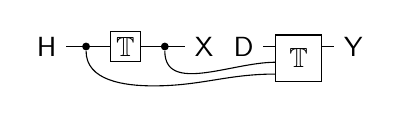
\begin{tikzpicture}
    \path (0,0) node (H) {$\RV{H}$}
     ++ (0.5,0) node[copymap] (copy0) {}
     ++ (0.5,0) node[kernel] (XH) {$\model{T}$}
     ++ (0.5,0) node[copymap] (copy1) {}
     ++ (0.5,0) node (X) {$\RV{X}$}
     ++ (0.5,0.) node (D) {$\RV{D}$}
     ++ (0.7,-0.15) node[kernel,inner sep=5pt] (YDXH) {$\model{T}$}
     ++ (0.7,0.15) node (Y) {$\RV{Y}$};
     \draw (H) -- (XH) -- (X) (D) to [out=0,in=180] ($(YDXH.west) + (0,0.15)$) ($(YDXH.east) + (0,0.15)$) -- (Y);
     \draw (copy0) to [out=-90,in=180] ($(copy0.east) + (0.8,-0.5)$) to [out=0,in=180] ($(YDXH.west) + (0,-0.2)$) (copy1) to [out=-90,in=180] ($(YDXH.west) + (0,-0.05)$);
\end{tikzpicture}\\
&= 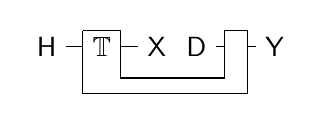
\begin{tikzpicture}
    \path (0,0) node (H) {$\RV{H}$}
     ++ (0.7,0) node (XH) {$\model{T}$}
     ++ (0.7,0) node (X) {$\RV{X}$}
     ++ (0.5,0) node (D) {$\RV{D}$}
     ++ (0.5,0) node[inner sep=4pt] (YDXH) {}
     ++ (0.5,0) node (Y) {$\RV{Y}$};
     \draw (H) -- (XH) -- (X) (D) -- (YDXH) -- (Y);
     \draw ($(XH.west) + (0,0.2)$) -- ($(XH.west) + (0,-0.6)$) -- ($(YDXH.east) + (0,-0.6)$)
     -- ($(YDXH.east) + (0,0.2)$) -- ($(YDXH.west) + (0,0.2)$) -- ($(YDXH.west) + (0,-0.4)$)
     -- ($(XH.east) + (0,-0.4)$) -- ($(XH.east) + (0,0.2)$) -- ($(XH.west) + (0,0.2)$);
\end{tikzpicture}\label{eq:kernel_with_hole}
\end{align}

We can take any strategy $\model{S}_\alpha[\RV{D}|\RV{X}]$ and drop it into the ``hole'' in \ref{eq:kernel_with_hole} (as described in Equation \ref{eq:see_do_query}) to get a forecast of the outcome of that strategy. 
%!TEX root = main.tex


\section{Variables and Probability Models}\label{sec:vague_variables}

\subsection{Semantics of observed and unobserved variables}\label{sec:variables}

We are interested in constructing \emph{probabilistic models} which explain some part of the world. In a model, variables play the role of ``pointing to the parts of the world the model is explaining''. Both observed an unobserved variables play important roles in causal modelling and we think it is worth clarifying what variables of either type refer to. Ultimately, our interpretation is largely the standard one: a probabilistic model is associated with an experiment or measurement procedure that yields values in a well-defined set. Observable variables are obtained by applying well-defined functions to the result of this total measurement. We explain how we can use a richer sample space that includes unobserved variables. Unobserved variables are formally modelled in exactly the same way as observed variables, but unlike observed variables we don't offer a standard interpretation of unobserved variables. 

Consider Newton's second law in the form $\proc{F}=\proc{MA}$ as a simple example of a model that relates variables $\proc{F}$, $\proc{M}$ and $\proc{A}$. As \citet{feynman_feynman_1979} noted, this law is incomplete -- in order to understand it, we must bring some pre-existing understanding of force, mass and acceleration as independent things. Furthermore, the nature of this knowledge is somewhat perculiar. Acknowledging that physicists happen to know a great deal about determining the forces on an object, it remains true that in order to actually say what the net force on a real object is, even a highly knowledgeable physicist will still have to go and do some measurements, and the result of such measurements will be a vector representing the net forces on that object.

This suggests that we can think about ``force'' $\proc{F}$ (or mass or acceleration) as a kind of procedure that we apply to a particular real world object and which returns a mathematical object (in this case, a vector). We will call $\proc{F}$ a \emph{procedure}. Our view of $\proc{F}$ is akin to \citet{menger_random_2003}'s notion of variables as ``consistent classes of quantities'' that consist of pairing between real-world objects and quantities of some type. Force $\proc{F}$ itself is not a well-defined mathematical thing, as measurement procedures are not mathematically well-defined. At the same time, the set of values it can return \emph{are} well-defined mathematical things. 

The fact that procedures return well-defined mathematical quantities allows us to define an operation akin to function composition. If I have a procedure $\proc{B}$ that takes values in some set $B$, and a function $f:B\to C$, define the ``composition'' $f\circ \proc{B}$ to be the procedure given by applying the procedure $\proc{B}$ and then applying $f$ to the result. For example, $\proc{MA}$ is the composition of $h:(x,y)\mapsto xy$ with $(\proc{M},\proc{A})$ that measures the mass and acceleration of the same object, and returns their values in an ordered pair.

One might whether there is also some kind of ``append'' operation that takes a standalone $\proc{M}$ and a standalone $\proc{A}$ and returns a procedure $(\proc{M},\proc{A})$. Unlike function composition, this would be an operation that acts on two procedures rather than a procedure and a function. Rather than attempt to define any operation of this type, we simply assume that somehow a procedure has been devised that measures everything of interest, which we will call $\proc{S}$ which takes values in $\Psi$. We assume $\proc{S}$ is such that any procedure of interest can be written as $f\circ \proc{S}$ for some $f$.

For the model $\proc{F}=\proc{MA}$, for example, we could assume $\proc{F}=f\circ \proc{S}$ for some $f$ and $(\proc{M},\proc{A})=g\circ \proc{S}$ for some $g$. In this case, we can get $\proc{MA}=h\circ(\proc{M},\proc{A})=(h\circ g)\circ\proc{S}$. Note that each procedure is associated with a unique function with domain $\Psi$.

Thus far, $\Psi$ is a ``sample space'' that only contains observable variables. To include unobserved variables, we posit a richer sample space $\Omega$ such that the measurement $\proc{S}$ determines an element of some partition of $\Omega$ rather than an element of $\Omega$ itself. Then, by analogy to procedures defined with respect to $\proc{S}$, we identify variables in general with measurable functions defined on the domain $\Omega$. 

Specifically, suppose $\proc{S}$ takes values in $\Psi$. Then we can propose a sample space $\Omega$ such that $|\Omega|\geq |\Psi|$ and a surjective function $\RV{S}:\Omega\to \Psi$ associated with $\proc{S}$. We connect $\Omega$, $\RV{S}$ and $\proc{S}$ with the notion of \emph{compatibility with obseravation}:

\begin{align}
 &\omega\in \Omega\text{ is \emph{compatible with observation} iff the result yielded by }S\text{ is equal to }\RV{S}(\omega)\label{def:observable}
\end{align}

Thus the procedure $\proc{S}$ eventually restricts the observationally compatible elements of $\Omega$ to some subset induced by $\RV{S}$; we may or may not add additional postulates to choose from the remaining candidates. A probability model on $\Omega$ could be regarded as a forecast of which elements of $\Omega$ are likely to be observationally compatible. If we have a formal variable $\RV{X}$ that can be written as $f\circ \RV{S}$ for some $f$, then $\RV{X}$ is an \emph{observed variable}, otherwise it is an \emph{unobserved variable}.

One thing to note in this setup is that two different sets of measurement outcomes $\Psi$ and $\Psi'$ entails specifying an different mesurement procedurees $\proc{S}$ and $\proc{S}'$. On the other hand, it is possible to define different sample spaces $\Omega$ and $\Omega'$ that share a single procedure $\proc{S}$ (recall that the procedure $\proc{S}$ does not itself depend on $\Omega$, though its model $\RV{S}$ does). We will sometimes consider different models of the same observable procedurees.

As far as we know, distinguishing variables from procedurees is somewhat nonstandard, but it is useful because, as we have discussed, every procedure is assumed to be modeled by a variable but not every variable is a model of a procedure. Furthermore, while they may not be distinguished, both variables and procedurees are often discussed in statistical texts. For example, \citet{pearl_causality:_2009} offers the following two, purportedly equivalent, definitions of variables:
\begin{quote}
By a \emph{variable} we will mean an attribute, measurement or inquiry that may take on one of several possible outcomes, or values, from a specified domain. If we have beliefs (i.e., probabilities) attached to the possible values that a variable may attain, we will call that variable a random variable.
\end{quote}

\begin{quote}
This is a minor generalization of the textbook definition, according to which a random variable is a mapping from the sample space (e.g., the set of elementary events) to the real line. In our definition, the mapping is from the sample space to any set of objects called ``values,'' which may or may not be ordered.
\end{quote}

Variables model procedurees, but they are not the same thing as procedurees.

\subsection{Events}

To recap, we have a procedure $\proc{S}$ yielding values in $\Psi$ that measures everything we are interested in, a sample space $\Omega$ and a function $\RV{S}$ that models $\proc{S}$ in the sense of Definition \ref{def:observable}. We assume also that $\Psi$ has a $\sigma$-algebra $\sigalg{E}$ (this may be the power set of $\Psi$, as measurement procedurees are typically limited to finite precision). $\Omega$ is equipped with a $\sigma$-algebra $\sigalg{F}$ such that $\sigma(\RV{S})\subset \sigalg{F}$. If a procedure $\proc{X}=f\circ \RV{S}$ then we define $\RV{X}:\Omega\to X$ by $\RV{X}:=f\circ\RV{S}$.

If a particular procedure $\proc{X}=f\circ \proc{S}$ eventually yields a value $x$, then the values of $\Omega$ compatible with observation are a subset of $\RV{X}^{-1}(x)$. We define $\RV{X}\bowtie x:\cong \RV{X}^{-1}(x)$, which we read ``$\RV{X}$ yields x''. This definition applies to all types of variables, not just observables, but we only provide an interpretation of the meaning of this definition when $\RV{X}$ is associated with $\proc{X}$: in that case, $\RV{X}\bowtie x$ contains the compatible values of $\Omega$ iff $\proc{X}$ yields x. 

We extend this to say, for measurable $A\in \sigalg{X}$, $\RV{X}\bowtie A=\bigcup_{x\in A} \RV{X}\bowtie x$. Given $\RV{Y}:\Omega\to X$, $\RV{X}\bowtie \RV{Y}=\bigcup_{x\in X} \RV{X}\bowtie x \cap \RV{Y}\bowtie x$, read ``$\RV{X}$ yields the same as $\RV{Y}$''. $\RV{X}\not\bowtie x:\cong (\RV{X}\bowtie x)^C$.

We use a bowtie to stand for ``yields'': $\RV{Y}\bowtie y :\cong \RV{Y}^{-1}(y)$. It is somewhat common to use the symbol ``$=$'' to do this job, but we do not want to do this because $\RV{Y}=y$ already has a meaning, namely that $\RV{Y}$ is a constant function everywhere equal to $y$. 

\subsection{Probabilistic models}

We've offered an interpretation of variables, but we won't offer a similar interpretation of probability. Interpreting probability is notoriously difficult. Incidentally, conditioning on different values of unobserved variables typically induces different probability models over observed variables, so supplying an interpretion of what it means for a probability model to be ``correct'' might also entail an interpretation of what it means for an unobserved variable to yield a particular value.

We will assume for the time being that we want to construct probabilistic models that relate collection of variables, defined as they have been above. The standard method for 

Throughout this paper, we will assume all measurable sets are finite sets. This is because it makes explanations simpler and because it is easy to show that conditional probabilities exist in this setting (Lemma \ref{lem:subm_exist}).

At this point we have a crude model of some observation procedure $\proc{S}$ given by $\Omega$ and a collection of variables, and we can relate a claim that some $\omega$ is \emph{compatible with observations} to real-world events via the procedure $\proc{S}$. We wish to extend this with probability distributions and conditional probabilties. A probability distribution $\prob{P}^{\RV{X}}$ for some variable $\RV{X}:\Omega\to B$ is a probability measure on $(B,\sigalg{B})$, and a conditional probability $\prob{P}^{\RV{X}|\RV{Y}}$ for $\RV{X}:\Omega\to B$, $\RV{Y}:\Omega\to C$ is a Markov kernel $B\kto C$. A a probability distribution $\mu$ on $(B,\sigalg{B})$ is a $\sigma$-additive measure $\mu:\sigalg{B}\to [0,1]$ such that $\mu(\emptyset)=0$ and $\mu(B)=1$, and a Markov kernel $\kernel{K}:B\kto C$ is a is a map $B\times \sigalg{C}\to [0,1]$ such that

\begin{itemize}
	\item x\mapsto \kernel{K}(x,A) is $\sigalg{B}$-measurable for all $A\in \sigalg{C}$
	\item A\mapsto \kernel{K}(x,A) is a probability measure on $(C,\sigalg{C})$ for all $x\in B$
\end{itemize}

Given $\prob{P}^{\RV{X}}$, we identify $\prob{P}^{\RV{X}}(\{x\})$ with the probability $\prob{P}(\RV{X}\bowtie x)$ of the event $\RV{X}\bowtie x$ under some related probability measure $\prob{P}$ on $(\Omega,\sigalg{F})$. That is, we assume that there exists some $\prob{P}$ on $(\Omega,\sigalg{F})$ such that $\prob{P}^{\RV{X}}(\{x\})=\prob{P}(\RV{X}\bowtie x)$. More generally, we say a collection of probability distributions $\{\prob{P}^{\RV{X}_i}|i\in D\}$ is \emph{sample space compatible} if there exists $\prob{P}$ on $\Omega$ such that $\prob{P}^{\RV{X}_i}(A)=\prob{P}(\RV{X}_i\bowtie A)$ for all $A\in \sigalg{B}$, $i\in D$.

Extending sample space compatibility to conditional probabilities is somewhat trickier, because conditional probably does not seem to have a simple correspondence to any more fundamental notion. See for example \citet{hajek_what_2003} for some difficulties with defining conditional probability purely in terms or a probability measure $\prob{P}$ on $(\Omega,\sigalg{F})$, and \citet{nguyen_probability_2002} for a difficulties with interpreting conditional probability as the probability of an implication.

We say a collection of conditional probabilities $\{\prob{P}^{\RV{X}_i|\RV{X}_j}|i\in D, j\in E\}$ is sample space compatible relative to $\RV{Y}$ if there exists some $\prob{P}^{;\RV{Y}}:Y\kto \Omega$ such that, for all $j\in E$, $i\in D$:

\begin{align}
	\RV{X}_i^{-1}(A)\cap \RV{X}_{j}^{-1}(b) &= \emptyset \implies \prob{P}^{\RV{X}_i|\RV{X}_j}(A|b)=0 &\forall A\in \sigalg{X}_i, b\in X_j \label{eq:ssc_1}\\
	\prob{P}^{;\RV{Y}}((\RV{X}_i,\RV{X}_j)\bowtie A\times B|c) &= \int_A \prob{P}^{\RV{X}_{i}|\RV{X}_j}(B|\RV{X}_j(\omega))\prob{P}^{;\RV{Y}}(d\omega|c) &\forall c\in Y:\prob{P}^{;\RV{Y}}(\RV{X}_j\bowtie A|c)>0 \label{eq:ssc_2}
\end{align}

$\{\prob{P}^{\RV{X}_i|\RV{X}_j}|i\in D, j\in E\}$ is sample space compatible if there is some $\RV{Y}$ such that it is sample space compatible relative to $\RV{Y}$. Note that Equation \ref{eq:ssc_2} is similar to a standard definition of conditional probability, while Equation \ref{eq:ssc_1} is an additional requirement, roughly saying ``the probability of $u$ given $\not u$ is always zero''. 

By convention, a collection of conditional probabilities with the same base letter $\prob{P}^{\RV{X}|\RV{Y}}$, $\prob{P}^{\RV{Z}|\RV{Y}}$ are held to be jointly sample space compatible.

Consider a model obtained from ``truncated factorisation'', an operation that is typical in causal modelling and atypical in probability theory. Suppose we have a causal Bayesian network $(\prob{P}^{\RV{XYZ}},\mathcal{G})$ where $\RV{X}:\Omega\to A$, $\RV{Y}:\Omega\to B$ and $\RV{Z}:\Omega\to C$ are variables, $\prob{P}^{\RV{XYZ}}$ is a probability measure on $A\times B\times C$ that we call ``a probability model of $(\RV{X},\RV{Y},\RV{Z})$'' and $\mathcal{G}$ is a Directed Acyclic Graph whose vertices we identify with $\RV{X}$, $\RV{Y}$ and $\RV{Z}$ that contains the edges $\RV{X}\longrightarrowRHD \RV{Y}$ and $\RV{X}\longleftarrowRHD \RV{Z} \longrightarrowRHD \RV{Y}$. ``Setting $\RV{X}$ to $x$'' is an operation that takes as inputs $\prob{P}^{\RV{XYZ}}$, $\mathcal{G}$ and some $x\in A$ and returns a new probability measure $\prob{P}_x^{\RV{XYZ}}$ on $A\times B\times C$ given by \citep[page ~24]{pearl_causality:_2009}:
\begin{align}
	\prob{P}^{\RV{XYZ}}_{x}(x',y,z)=\prob{P}^{\RV{Y|XZ}}(y|x,z)\prob{P}^{\RV{Z}}(z)\llbracket x=x' \rrbracket\label{eq:truncated_fac}
\end{align}

Equation \ref{eq:truncated_fac} embodies three assumptions about a model of the operation of ``setting $\RV{X}$ to $x$''. First, such a model must assign probability 1 to the proposition that $\RV{X}$ yields $x$. Second, such a model must assign the same marginal probability distribution to $\RV{Z}$ as the input distribution; $\prob{P}^{\RV{Z}}=\prob{P}_{x}^{\RV{Z}}$. Finally, our model must also assign the same conditional probability to $\RV{Y}$ given $\RV{X}$ and $\RV{Z}$; $\prob{P}^{\RV{Y}|\RV{XZ}}=\prob{P}_x^{\RV{Y}|\RV{XZ}}$.

We cannot always find a sensible probability distribution $\prob{P}_x^{\RV{XYZ}}$ that has the required properties. For example, if $\RV{X}$ and $\RV{Z}$ happen to be represented by the same function -- which is to say, the underlying procedurees $X$ and $Z$ both refer to the same measurement of the same thing -- then any model must surely assign probability 1 to the event $\RV{X}\bowtie \RV{Z}$; or equivalently, probability 0 to the event $\RV{X}\not\bowtie \RV{Z}$. However, this cannot be done in accordance with Equation \ref{eq:truncated_fac} for all $x\in A$ if $|A|\geq 2$. This is because for $x\neq x'\in A$, $\prob{P}_x^{\RV{X}}\neq \prob{P}_{x'}^{\RV{X}}$ but $\prob{P}_x^{\RV{Z}}=\prob{P}_{x'}^{\RV{Z}}$.

Thus we have \emph{four} assumptions to satisfy:
\begin{enumerate}
	\item $\prob{P}_x^{\RV{X}}=1$
	\item $\prob{P}^{\RV{Z}}=\prob{P}_{x}^{\RV{Z}}$
	\item $\prob{P}^{\RV{Y}|\RV{XZ}}=\prob{P}_x^{\RV{Y}|\RV{XZ}}$
	\item If $\RV{X}=\RV{Z}$ then $\prob{P}_x(\RV{X}\bowtie \RV{Z})=1$
\end{enumerate}

Crucially, only assumptions 2 and 3 depend on the assumed causal graph $\mathcal{G}$; assumptions 1 and 4 should hold regardless. As we will show, these assumptions are both implied by the assumption that we have some $\prob{Q}^{\RV{XYZ}|\RV{X}}$ that is \emph{sample space compatible} such that $\prob{P}^{\RV{XYZ}}_x(x',y,z) = \prob{Q}^{\RV{XYZ}|\RV{X}}(x',y,z|x)$. Furthermore, as we will show, Equation \ref{eq:ssc_1} implies assumption 1 and Equation \ref{eq:ssc_2} implies assumption 4, and so both requirements are needed.

The example of $\RV{X}=\RV{A}$ might seem absurd. Consider instead $\RV{Z}=(\RV{H},\RV{W})$, representing the height in metres and weight in kilograms of a particular person, and $\RV{X}$ represents their body mass index, which is to say $\RV{X}=\frac{\RV{W}}{\RV{H}^2}$ (not that in both cases we are using ``$=$'', which means these variables are \emph{equal as functions}, not that they \emph{yield the same result with probability 1}, which would involve the symbol ``$\bowtie$''). A causal graph with exactly these variables and arrows analogous to ours appears in \citet{shahar_association_2009}. However, generally there is no $\prob{P}_x^{\RV{XHW}}$ that satisfies both $\RV{X}\bowtie \frac{\RV{W}}{\RV{H}^2}$ with probability 1 and Equation \ref{eq:truncated_fac}. This is true, for example, whenever $\prob{P}^{\RV{X}}$ has support at more than one point.

\subsection{Operating on Markov kernels with string diagrams}
Markov categories are abstract categories that represent models of the flow of information. Operations like Equation \ref{eq:truncated_fac} are expressible as abstract compositions in Markov categories, and may be represented with string diagrams developed for reasoning about objects in the category. Valid proofs using string diagrams correspond to valid theorems in \emph{any} Markov category, though we will limit our attention to the category of finite sets and Markov kernels in this paper. The main drawback of Markov categories is that, as they exist at the moment, they have no notion of ``variables''. More comprehensive introductions to Markov categories can be found in \citet{fritz_synthetic_2020,cho_disintegration_2019}.

Given measurable sets $(X,\sigalg{X})$ and $(Y,\sigalg{Y})$, a Markov kernel or stochastic map is a map $\kernel{K}:X\times \sigalg{Y}\to [0,1]$ such that

\begin{itemize}
	\item The map $x\mapsto \kernel{K}(x,A)$ is $\sigalg{X}$-measurable for every $A\in \sigalg{Y}$
	\item The map $A\mapsto \kernel{K}(x,A)$ is a probability measure for every $x\in X$
\end{itemize}

Where $X$ and $Y$ are finite sets with the discrete $\sigma$-algebra, we can represent a Markov kernel $\kernel{K}$ as a $|X|\times |Y|$ matrix where $\sum_{y\in Y} \kernel{K}_x^y = 1$ for every $x\in X$. We will give Markov kernels the signature $\kernel{K}:X\kto Y$ to indicate that they map from $X$ to probability distributions on $Y$.

Graphically, Markov kernels are drawn as boxes with input and output wires, and probability measures (which are kernels with the domain $\{*\}$) are represented by triangles:

\begin{align}
\kernel{K}&:=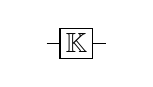
\begin{tikzpicture}[baseline={([yshift=-.5ex]current bounding box.center)}]
	\path (0,0) node (A) {}
	++ (0.5,0) node[kernel] (K) {$\kernel{K}$}
	++ (0.5,0) node (B) {};
	\draw (A) -- (K) -- (B);
\end{tikzpicture}\\
\kernel{P}&:= 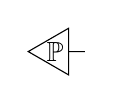
\begin{tikzpicture}[baseline={([yshift=-.5ex]current bounding box.center)}]
	\path (0,0) node[dist] (K) {$\kernel{P}$}
	++ (0.5,0) node (B) {};
	\draw (K) -- (B);
\end{tikzpicture}
\end{align}

Two Markov kernels $\kernel{L}:X\kto Y$ and $\kernel{M}:Y\kto Z$ have a product $\kernel{L}\kernel{M}:X\kto Z$ given by the matrix product $\kernel{L}\kernel{M}_x^z = \sum_y \kernel{L}_x^y\kernel{M}_y^z$. Graphically, we write represent by joining wires together:

\begin{align}
	\kernel{L}\kernel{M}:= 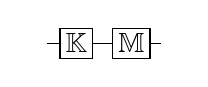
\begin{tikzpicture}[baseline={([yshift=-.5ex]current bounding box.center)}]
	\path (0,0) node (A) {}
	++ (0.5,0) node[kernel] (K) {$\kernel{K}$}
	++ (0.7,0) node[kernel] (M) {$\kernel{M}$}
	++ (0.5,0) node (B) {};
	\draw (A) -- (K) -- (M) -- (B);
\end{tikzpicture}
\end{align}

The Cartesian product $X\times Y:=\{(x,y)|x\in X, y\in Y\}$. Given kernels $\kernel{K}:W\kto Y$ and $\kernel{L}:X\kto Z$, the tensor product $\kernel{K}\otimes\kernel{L}:W\times X\kto Y\times Z$ is defined by $(\kernel{K}\otimes\kernel{L})_{(w,x)}^{(y,z)}:=K_{w}^y L_{x}^z$ and represents applying the kernels in parallel to their inputs.

The tensor product is represeted by drawing kernels in parallel:

\begin{align}
	\kernel{K}\otimes \kernel{L}&:=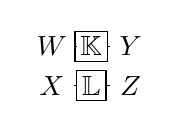
\begin{tikzpicture}[baseline={([yshift=-.5ex]current bounding box.center)}]
	\path (0,0) node (A) {$W$}
	++ (0.5,0) node[kernel] (K) {$\kernel{K}$}
	++ (0.5,0) node (B) {$Y$};
	\path (0,-0.5) node (C) {$X$}
	++ (0.5,0) node[kernel] (L) {$\kernel{L}$}
	++ (0.5,0) node (D) {$Z$};
	\draw (A) -- (K) -- (B);
	\draw (C) -- (L) -- (D);
\end{tikzpicture}
\end{align}

We read diagrams from left to right (this is somewhat different to \citet{fritz_synthetic_2020,cho_disintegration_2019,fong_causal_2013} but in line with \citet{selinger_survey_2010}). A diagram describes products and tensor products of Markov kernels, which are expressed according to the conventions described above. There are a collection of special Markov kernels for which we can replace the generic ``box'' of a Markov kernel with a diagrammatic elements that are visually suggestive of what these kernels accomplish.

A description of these kernels follows.

The identity map $\text{id}_X:X\kto X$ defined by $(\text{id}_X)_x^{x'}= \llbracket x = x' \rrbracket$, where the iverson bracket $\llbracket \cdot \rrbracket$ evaluates to $1$ if $\cdot$ is true and $0$ otherwise, is a bare line:

\begin{align}
	\mathrm{id}_X&:=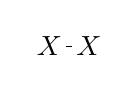
\begin{tikzpicture}[baseline={([yshift=-.5ex]current bounding box.center)}]
	\path (0,0) node (A) {$X$} ++ (0.5,0) node (B) {$X$};
	\draw (A) -- (B);
\end{tikzpicture}
\end{align}

We choose a particular 1-element set $\{*\}$ that acts as the identity in the sense that $\{*\}\times A=A\times \{*\} = A$ for any set $A$. The erase map $\text{del}_X:X\kto \{*\}$ defined by $(\text{del}_X)_x^* = 1$ is a Markov kernel that ``discards the input'' (we will later use it for marginalising joint distributions). It is drawn as a fuse:

\begin{align}
	\text{del}_X&:=\begin{tikzpicture}[baseline={([yshift=-.5ex]current bounding box.center)}]
	\path (0,0) ++ (1,0) node (B) {$X$};
	\draw[-{Rays[n=8]}] (A) -- (B);
\end{tikzpicture}
\end{align}

The copy map $\text{copy}_X:X\kto X\times X$ defined by $(\text{copy}_X)_x^{x',x''}=\llbracket x=x' \rrbracket \llbracket x=x'' \rrbracket$ is a Markov kernel that makes two identical copies of the input. It is drawn as a fork:

\begin{align}
	\text{copy}_X&:=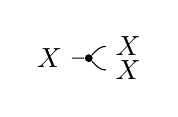
\begin{tikzpicture}[baseline={([yshift=-.5ex]current bounding box.center)}]
	\path (0,0) node (A) {$X$} 
	++ (0.5,0) node[copymap] (copy0) {}
	++ (0.5,0.15) node (B) {$X$}
	+ (0,-0.3) node (C) {$X$};
	\draw (A) -- (copy0) to [out=45,in=180] (B) (copy0) to [out=-45, in=180] (C);
\end{tikzpicture}
\end{align}

The swap map $\text{swap}_{X,Y}:X\times Y\kto Y\times X$ defined by $(\text{swap}_{X,Y})_{x,y}^{y',x'}=\llbracket x=x' \rrbracket\llbracket y=y' \rrbracket$ swaps two inputs, and is represented by crossing wires:

\begin{align}
	\text{swap}_X &:=  
\begin{tikzpicture}[baseline={([yshift=-.5ex]current bounding box.center)}]
		\path (0,0) node (A) {} 
		+ (0,-0.5) node (B) {}
		++ (1,0) node (C) {}
		+ (0,-0.5) node (D) {};
		\draw (A) to [out=0,in=180] (D) (B) to [out=0, in=180] (C);
	\end{tikzpicture}
\end{align}

Because we anticipate that the graphical notation will be unfamiliar to many, we will also include translations to more familiar notation.

\subsection{Truncated factorisation with Markov kernels}

The Markov kernels introduced in the previous section can be though of as ``conditional probability distributions without variables''. We can use these to represent an operation very similar to Equation \ref{eq:truncated_fac}. Note that $P^{\RV{Y|XZ}}$ must be represented by a Markov kernel $\kernel{K}:X\times Z\kto Y$ and $\prob{P}^{\RV{Z}}$ by a Markov kernel $\kernel{L}\in \Delta(Z)$. Then we can define a Markov kernel $\kernel{M}:X\kto X\times Z$ representing $x\mapsto \prob{P}^{\RV{YZ}}_{x}(y,z)$ by

\begin{align}
	\kernel{M}:= \tikzfig{truncated_factorisation}\label{eq:tfac_setted}
\end{align}

There is, however, a key difference between Equation \ref{eq:tfac_setted} and Equation \ref{eq:truncated_fac}: the Markov kernels in the latter equation describe the distribution of particular variables, while the former equation describes Markov kernels only.

To illustrate why we need variables, consider an arbitrary Markov kernel $\kernel{K}:\{*\}\kto \Delta(X\times X)$. We could draw this:
\begin{align}
	\kernel{K}:= \tikzfig{double_label}\label{eq:double_label}
\end{align}
We label both wires with the set $X$. However, say $X=\{0,1\}$. Then $\kernel{K}$ could be the kernel $\kernel{K}^{x_1,x_2} = \llbracket x_1 = 0\rrbracket \llbracket x_2 = 1\rrbracket$. In this case, both of its outputs must represent \emph{different} variables, despite taking values in the same set. On the other hand, if $\kernel{K}^{x_1,x_2} = 0.5 \llbracket x_1 = x_2 \rrbracket$ then both outputs coudl represent the same variable, because they are deterministically the same, or they could represent different variables that happen to be equal. We need some way to distinguish the two cases.


\subsection{Composition and probability with variables}

Our goal is to define a category of ``finite sets and Markov kernels with variables''. Introducing variables requires an assumption of consistency, which we don't know how to express in category theoretic terms. Our approach is to define a category of Markov kernels with variables that may or may not be consistent, which we will need to check for the resulting models. Because the consistency assumption is not expressed category theoretically, many proofs in this section only apply to our chosen setting of finite sets.

\begin{definition}[Variable]
Given a \emph{sample space} $\Omega$, a variable $f_\RV{X}$ is a function $\Omega\to A$ where $A$ is a vector space. We will also refer to the associated Markov kernel $\RV{X}:\Omega\kto A$
as a variable, where $\RV{X}_x^a=\llbracket a = f_{\RV{X}}(x) \rrbracket$.
\end{definition}

We define the \emph{product} of two variables as follows:
\begin{itemize}
	\item \textbf{Product:} Given variables $\RV{W}:\Omega\kto A$ and $\RV{V}:\Omega\kto B$, the product is defined as $(\RV{W}, \RV{V})=\text{copy}_{\Omega} (\RV{W}\otimes\RV{V})$
\end{itemize}

The \emph{unit} variable is the erase map $\RV{I}:=\text{del}_\Omega$, with $(\RV{I},\RV{X})=(\RV{X},\RV{I})=\RV{X}$ (up to isomorphism) for any $\RV{X}$.

We then need a notion of Markov kernels that ``maps between variables''. An \emph{indexed Markov kernel} is such a thing.

\begin{definition}[Indexed Markov kernel]
Given variables $\RV{X}:\Omega\to A$ and $\RV{Y}:\Omega\to B$, an indexed Markov kernel $\kernel{K}:\RV{X}\kto \RV{Y}$ is a triple $(\kernel{K}',\RV{X},\RV{Y})$ where $\kernel{K}':A\kto B$ is the \emph{underlying kernel}, $\RV{X}$ is the \emph{input index} and $\RV{Y}$ is the \emph{output index}.
\end{definition}

For example, if $\kernel{K}:(\RV{A}_1,\RV{A}_2)\to \Delta(\RV{B}_1,\RV{B}_2)$, for example, we can draw:

\begin{align}
	\kernel{K} := 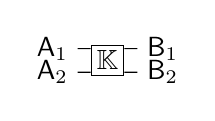
\begin{tikzpicture}[baseline={([yshift=-.5ex]current bounding box.center)}]
	\path (0,0) node (A1) {$\RV{A}_1$}
	+ (0,-0.3) node (A2) {$\RV{A}_2$}
	++ (0.7,-0.15) node[kernel] (K) {$\kernel{K}$}
	++ (0.7,0.15) node (B1) {$\RV{B}_1$}
	+ (0,-0.3) node (B2) {$\RV{B}_2$};
	\draw (A1) -- ($(K.west) + (0,0.15)$) (A2) -- ($(K.west) + (0,-0.15)$);
	\draw (B1) -- ($(K.east) + (0,0.15)$) (B2) -- ($(K.east) + (0,-0.15)$);
\end{tikzpicture}
\end{align}

or

\begin{align}
	\kernel{K} = 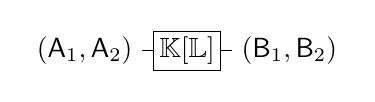
\begin{tikzpicture}[baseline={([yshift=-.5ex]current bounding box.center)}]
	\path (0,0) node (A1) {$(\RV{A}_1,\RV{A}_2)$}
	++ (1.3,0) node[kernel] (K) {$\kernel{K}[\model{L}]$}
	++ (1.3,0.) node (B1) {$(\RV{B}_1,\RV{B}_2)$};
	\draw (A1) -- (K) -- (B1);
\end{tikzpicture}
\end{align}

We define the product of indexed Markov kenrnels $\kernel{K}:\RV{X}\kto \RV{Y}$ and $\kernel{L}:\RV{Y}\kto \RV{Z}$ as the triple $\kernel{K}\kernel{L}:=(\kernel{K}'\kernel{L}',\RV{X},\RV{Z})$.

Similarly, the tensor product of $\kernel{K}:\RV{X}\kto\RV{Y}$ and $\kernel{L}:\RV{W}\kto\RV{Z}$ is the triple $\kernel{K}\otimes\kernel{L}:=(\kernel{K}'\otimes\kernel{L}',(\RV{X},\RV{W}),(\RV{Y},\RV{Z}))$.

We define $\text{Id}_{\RV{X}}$ to be the model $(\text{Id}_X,\RV{X},\RV{X})$, and similarly the indexed versions $\text{del}_{\RV{X}}$, $\text{copy}_{\RV{X}}$ and $\text{swap}_{\RV{X},\RV{Y}}$ are obtained by taking the unindexed versions of these maps and attaching the appropriate random variables as indices. Diagrams are the diagrams associated with the underlying kernel, with input and output wires annotated with input and output indices.

The category of indexed Markov kernels as morphisms and variables as objects is a Markov category (Appendix \ref{sec:app_mcat}), and so a valid derivation based on the string diagram language for Markov categories corresponds to a valid theorem in this category. However, most of the diagrams we can form are not viable candidates for models of our variables. For example, if $\RV{X}$ takes values in $\{0,1\}$ we can propose an indexed Markov kernel $\kernel{K}:\RV{X}\kto\RV{X}$ with $\kernel{K}_a^{\prime b}=0.5$ for all $a, b$. However, this is not a useful model of the variable $\RV{X}$ -- it expresses something like ``if we know the value of $\RV{X}$, then we belive that $\RV{X}$ could take any value with equal probability''.

We define a \emph{model} as ``an indexed Markov kernel that assigns probability 0 to things known to be contradictions''. A contradiction is a simultaneous assignment of values to the variables $\RV{X}$ and $\RV{Y}$ such that there is no value of $\omega$ under which they jointly take these values. Unless the value assignment to the domain variable is itself contradictory, we hold that any valid model must assign probability zero to such occurrences.

\begin{definition}[Probabilistic model]
An indexed Markov kernel $(\kernel{K}',\RV{X},\RV{Y})$ is a \emph{probabilistic model} (``model'' for short) if it is \emph{consistent}, which means it assigns probability 0 to contradictions:
\begin{align}
	f_{\RV{X}}^{-1}(a)\cap f_{\RV{Y}}^{-1}(b) = \emptyset \implies \left(\kernel{K}_{a}^{\prime b} = 0\right) \lor \left(f_{\RV{X}}^{-1}(a) = \emptyset\right)
\end{align}
A \emph{probability model} is a model where the underlying kernel $\kernel{K}'$ has the unit $\RV{I}$ as the domain. We use the font $\model{K}$ to distinguish models from arbitrary indexed Markov kernels.
\end{definition}

Consistency implies that for any $\model{K}:\RV{X}\kto\RV{Y}$, if $f_{\RV{Y}}=g\circ f_{\RV{X}}$ then $\model{K}_x^{g(x)}=1$. A particularly simple case of this is a model $\model{L}:\RV{X}\kto\RV{X}$, which must be such that $\model{L}_x^x=1$. \citet{hajek_what_2003} has pointed out that standard definitions of conditional probability allow the conditional probability to be arbitrary on a set of measure zero, even though ``the probability $\RV{X}=x$, given $\RV{X}=x$'' should obviously be 1.

We take the idea of marginal distributions as fundamental.

\begin{definition}[Marginal distribution]
Given a model $\model{K}:\RV{X}\kto(\RV{Y},\RV{Z})$, the marginal distribution of $\RV{Y}$, written $\model{K}^{\RV{Y}|\RV{X}}$, is obtained by marginalising over $\RV{Z}$:
\begin{align}
	\model{K}^{\RV{Y}|\RV{X}} &:= \tikzfig{marginal}\\
	&\iff\\
	(\model{K}^{\RV{Y}|\RV{X}})_x^y &= \sum_{z\in Z} \kernel{K}_x^{\prime yz}
\end{align}
\end{definition}

\begin{definition}[Disintegration]
Given a model $\model{K}:\RV{X}\kto(\RV{Y},\RV{Z})$, a disintegration $\model{L}:(\RV{X},\RV{Y})\kto \RV{Z}$ $\RV{Y}$, written $\model{K}^{\RV{Y}|\RV{X}}$, is obtained by marginalising over $\RV{Z}$
\end{definition}

We can always get a valid model by adding a copy map to a valid model, and conversely all valid models with repeated codomain variables must contain copy maps.

\begin{lemma}[Output copies of the same variable are identical]\label{lem:nocopy1}
For any $\kernel{K}:\RV{X}\kto (\RV{Y},\RV{Y},\RV{Z})$, $\kernel{K}$ is a model iff there exists some $\model{L}:\RV{X}\kto (\RV{Y},\RV{Z})$ such that
\begin{align}
		\kernel{K} &= \tikzfig{compose_with_copymap}\\
		&\iff \\
		\kernel{K}_{x}^{\prime y,y',z} &= \llbracket y=y' \rrbracket\kernel{L}_{x}^{\prime y,z}\\
\end{align}
\end{lemma}


\begin{proof}
$\implies$
For any $\omega,x,y,y',z$:
\begin{align}
	(\RV{X},\RV{Y},\RV{Y},\RV{Z})_\omega^{x,y,y',z} &= \llbracket f_{\RV{Y}}(\omega)=y \rrbracket \llbracket f_{\RV{Y}}(\omega)=y' \rrbracket (\RV{X},\RV{Z})_\omega^{x,z} \\
	&= \llbracket y=y' \rrbracket \llbracket f_{\RV{Y}}(\omega)=y \rrbracket(\RV{X},\RV{Z})_\omega^{x,z}
\end{align}
Therefore, by consistency, for any $x,y,y',z$, $y\neq y'\implies \kernel{K}_{x}^{\prime yy'z}=0$. Define $\kernel{L}$ by $\kernel{L}_x^{\prime y, z} := \kernel{K}_x^{\prime y y z}$. The fact that $\model{L}$ is a model follows from the assumption that $\model{K}$ is. Then
\begin{align}
	\kernel{K}_{x}^{\prime y,y',z} &= \llbracket y=y' \rrbracket\kernel{L}_{x}^{\prime y,z}
\end{align}
$\Leftarrow$
If $\model{L}$ is a model, then for any $x,x',y,z$, 
\begin{align}
\llbracket y=y'\rrbracket \model{L}_{x}^{\prime y,z}>0&\implies y=y'\land \model{L}_{x}^{\prime y,z}>0\\
													  &\implies \left(f_{\RV{X}}^{-1}(x)=\emptyset \right)\lor \left(f_{\RV{X}}^{-1}(x)\cap f_{\RV{Y}}^{-1}(y) \cap f_{\RV{Y}}^{-1}(y)\cap f_{\RV{Z}}^{-1}(z)\neq\emptyset \right)\\
\end{align}
\end{proof}

We can always get a valid model by copying the input to the output of a valid model, and conversely all valid models where there is a variable shared between the input and the output must copy that input to the output.

\begin{lemma}[Copies shared between input and output are identical]\label{lem:nocopy2}
For any $\kernel{K}:(\RV{X},\RV{Y})\kto (\RV{X},\RV{Z})$, $\kernel{K}$ is a model iff there exists some $\model{L}:(\RV{X},\RV{Y})\kto \RV{Z}$ such that
\begin{align}
	 \kernel{K} &= \tikzfig{precompose_with_copymap}\\
	 &\iff\\
	 \kernel{K}_{x,y}^{\prime x',z} &= \llbracket x=x'\rrbracket \kernel{L}_{\prime x,y}^{z}
\end{align}
\end{lemma}

\begin{proof}
$\implies$
For any $\omega,x,y,y',z$:
\begin{align}
	(\RV{X},\RV{Y},\RV{Y},\RV{Z})_\omega^{x,y,y',z} &= \llbracket f_{\RV{Y}}(\omega)=y \rrbracket \llbracket f_{\RV{Y}}(\omega)=y' \rrbracket (\RV{X},\RV{Z})_\omega^{x,z} \\
	&= \llbracket y=y' \rrbracket \llbracket f_{\RV{Y}}(\omega)=y \rrbracket(\RV{X},\RV{Z})_\omega^{x,z}
\end{align}
Therefore, by consistency, for any $x,y,y',z$, $x\neq x'\implies \model{K}_{x,y}^{\prime x'z}=0$. Define $\kernel{L}$ by $\kernel{L}_{x,y}^{\prime x', z} := \model{K}_{x,y}^{\prime x, y}$. The fact that $\kernel{L}$ is a model follows from the assumption that $\model{K}$ is a model. Then
\begin{align}
	\kernel{K}_{x, y}^{\prime x', z} &= \llbracket x=x' \rrbracket\kernel{L}_{x,y}^{\prime z}
\end{align}
$\Leftarrow$
If $\model{L}$ is a model, then for any $x,x',y,z$, 
\begin{align}
\llbracket x=x'\rrbracket \model{L}_{ x,y}^{\prime z}>0&\implies x=x'\land \model{L}_{ x,y}^{\prime z}>0\\
													  &\implies \left( f_{\RV{X}}^{-1}(x)\cap f_{\RV{Y}}^{-1}(y)=\emptyset \right)\lor \left(f_{\RV{X}}^{-1}(x)\cap f_{\RV{X}}^{-1}(x)\cap f_{\RV{Y}}^{-1}(y)\cap f_{\RV{Z}}^{-1}(z)\neq\emptyset \right)\\
\end{align}
\end{proof}

Consistency along with the notion of marginal distributions implies that, given some $\RV{X}$ and some $\model{K}:\RV{Y}\kto\text{Id}_\Omega$, the pushforward $\model{K}\model{X}$ is the unique model $\RV{Y}\kto \RV{X}$ that can be paired (Definition \ref{def:pairing}) with $\model{K}$. This is shown in Lemma \ref{lem:pushforward}.

\begin{lemma}[Uniqueness of models with the sample space as a domain]\label{lem:uniq_model}
For any $\RV{X}:\Omega\to A$, there is a unique model $\model{X}:\text{Id}_\Omega\kto \RV{X}$ given by $\model{X}:=(\RV{X},\text{Id}_\Omega,\RV{X})$.
\end{lemma}

\begin{proof}
$\RV{X}$ is a Markov kernel mapping from $\Omega\to A$, so it is a valid underlying kernel for $\model{X}$, and $\model{X}$ has input and output indices matching its signature. We need to show it satisfies consistency.

For any $\omega\in \Omega$, $a\in A$
\begin{align}
	\max_{\omega\in \Omega}(\text{Id}_\Omega,\RV{X})_{\omega}^{\omega',a} &= \max_{\omega\in \Omega} \llbracket \omega = \omega' \rrbracket \llbracket \omega = f_{\RV{X}}(a) \rrbracket\\
	&= \llbracket \omega = f_{\RV{X}}(a) \rrbracket\\
	&= \kernel{X}_\omega^a
\end{align}
Thus $\model{X}$ satisfies consistency.

Suppose there were some $\model{K}:\text{Id}_\Omega\kto \RV{X}$ not equal to $\RV{X}$. Then there must be some $\omega\in \Omega$, $b\in A$ such that $\model{K}_\omega^b\neq 0$ and $f_{\RV{X}}(\omega)\neq b$. Then
\begin{align}
	\max_{\omega\in \Omega}(\text{Id}_\Omega,\RV{X})_{\omega}^{\omega',a} &= \max_{\omega\in \Omega} \llbracket \omega = \omega' \rrbracket \llbracket \omega = f_{\RV{X}}(b) \rrbracket\\
	&= \llbracket \omega = f_{\RV{X}}(b) \rrbracket\\
	&= 0\\
	&< \model{K}_\omega^b
\end{align}
Thus $\model{K}$ doesn't satisfy consistency.
\end{proof}

% \begin{corollary}[Uniqueness of joint models]\label{cor:uniq_joint}
% For any $\RV{X}:\Omega\to A$, there is a unique model $\model{X}:\text{Id}_\Omega\kto (\RV{X},\text{Id}_{\Omega})$.
% \end{corollary}

% \begin{proof}
% Apply Lemma \ref{lem:nocopy2} to the model $\model{X}$ from Lemma \ref{lem:uniq_model}.
% \end{proof}

\begin{definition}[Pairing]\label{def:pairing}
Two models $\model{K}:\RV{X}\kto \RV{Y}$ and $\model{L}:\RV{X}\kto \RV{Z}$ can be \emph{paired} if there is some $\model{M}:\RV{X}\kto (\RV{Y},\RV{Z})$ such that $\model{K}=\model{M}^{\RV{Y}|\RV{X}}$ and $\model{L}=\model{M}^{\RV{Z}|\RV{X}}$.
\end{definition}

\begin{lemma}[Pushforward model]\label{lem:pushforward}
Given any model $\model{K}:\RV{Y}\kto \text{Id}_\Omega$ and any $\RV{X}$, there is a unique $\model{L}:\RV{Y}\kto \RV{X}$ that can be paired with $\model{K}$, and it is given by $(\kernel{L}^a_b = \sum_{\omega\in f_{\RV{X}}^{-1}(a)} \kernel{K}_b^{\omega}$.
\end{lemma}

\begin{proof}
Suppose that there is some $\model{L}$ that can be paired with $\model{K}$ via some $\model{M}:\RV{Y}\kto(\text{Id}_\Omega,\RV{X})$. Then, by the existence of disintegrations, there must be some $\model{N}:\text{Id}_{\Omega}\kto \RV{X}$ such that
\begin{align}
	\model{M}&=\tikzfig{disintegration_omega}
\end{align}
By Corollary \ref{cor:uniq_joint}, there is only one model $\model{N}:\text{Id}_{\Omega}\kto \RV{X}$ is unique and equal to $\model{X}:=(\RV{X},\text{Id}_\Omega,\RV{X})$.

It remains to be shown that $\model{M}$ is also a model. We already know that $\model{K}$ is consistent with respect to $(\RV{Y},\text{Id}_\Omega)$ and $\model{L}$ is consistent with respect to $(\text{Id}_\Omega,\RV{X})$. $\model{M}$ must be consistent with respect to $(\RV{Y},\text{Id}_\Omega,\RV{X})$. Consider any $x\in X$, $\omega\in \Omega$, $y\in Y$ such that $f_{\RV{X}}^{-1}(x)\cap \{\omega\}\neq \emptyset$ and $f_{\RV{Y}}^{-1}(y)\cap\{\omega\}\neq \emptyset$. Trouble might arise if $f_{\RV{X}}^{-1}(x)\cap \{\omega\} \cap f_{\RV{Y}}^{-1}(y)=\emptyset$, but this is obviously impossible as $\omega\in f_{\RV{X}}^{-1}(x)$ and $\omega\in f_{\RV{Y}}^{-1}(y)$.

Finally, for any $a\in A$, $b\in B$
\begin{align}
	(\model{K}\model{X})^a_b &= \sum_{\omega\in \Omega} \model{P}_b^\omega\RV{X}_\omega^a\\
						 &= \sum_{\omega\in \Omega} \model{P}_b^\omega \llbracket a = f_{\RV{X}}(\omega) \rrbracket\\
						 &= \sum_{\omega\in f^{-1}(a)} \model{P}_b^{\omega}
\end{align}
\end{proof}

\begin{corollary}[Pushforward probability model]\label{corr:pushforward}
Given any probability model $\model{P}:\RV{I}\kto \text{Id}_\Omega$, there is a unique model $\model{P}^{\RV{X}}:\RV{I}\kto \RV{X}$ such that $\model{P}^{\RV{X}}=\model{P}\model{Q}$ for some $\model{Q}:\text{Id}_\Omega\to \RV{X}$, and it is given by $(\model{P}^{\RV{X}})^a_b = \sum_{\omega\in f^{-1}(a)} \model{P}_b^{\omega}$.
\end{corollary}

\begin{proof}
Apply Lemma \ref{lem:pushforward} to a model $\model{P}:\RV{I}\kto\text{Id}_{\Omega}$.
\end{proof}

The following lemmas can help us check whether an indexed Markov kernel is a valid model.



We take the following term from \citet{constantinou_extended_2017}. Our definition is equivalent to unconditional variation independence in that paper.

\begin{definition}[Variation independence]
Two variables $\RV{X}:\Omega\kto X$ and $\RV{Y}:\Omega\kto Y$ are variation independent, written $\RV{X}\perp_v \RV{Y}$, if for all $y\in f_\RV{Y}(\Omega)R(f_{\RV{Y}})$
\begin{align}
 f_\RV{Y}(\Omega) \times f_{\RV{X}}(\Omega) = \{(f_{\RV{Y}}(\omega),f_{\RV{X}}(\omega))|\omega\in \Omega\}
\end{align}
\end{definition}

If a collection of variables is variation independent and surjective, then an arbitrary indexed Markov kernel labelled with these variables is a model.

\begin{lemma}[Consistency via variation conditional independence]\label{lem:var_indep}
Given an indexed Markov kernel $\kernel{K}:\RV{X} \kto \RV{Y}$ with $\RV{X}:\Omega\kto X$ and $\RV{Y}:\Omega\kto Y$, if $f_\RV{Y}$ is surjective and $\RV{Y}\perp_v \RV{X}$ then $\kernel{K}$ is a model.
\end{lemma}

\begin{proof}
By variation independence and surjectivity of $f_{\RV{Y}}$, for any $x\in X$, $y\in Y$, $f_{\RV{X}}^{-1}(x)\cap f_{\RV{Y}}^{-1}(y) = \emptyset \implies f_{\RV{X}}^{-1}(x) = \emptyset$. Thus the criterion of consistency places no restrictions on $\kernel{K}$.
\end{proof}

\todo[inline]{I think Lemmas \ref{lem:nocopy1} and \ref{lem:nocopy2} might be sufficient to offer diagrammatic checks of consistency if all variables that are not identical are variation independent. This is probably an interesting result, but I'm not sure if it's a higher priority than filling out the rest of the content.}

Alternatively, if we have a strictly positive indexed Markov kernel that is known to be a model, we can conclude that arbitrary indexed Markov kernels with appropriate labels are also models.

\begin{lemma}[Consistency via positive models]\label{lem:avoid_contradic}
Given a model $\model{K}:\RV{X}\kto (\RV{Y},\RV{Z})$, if an indexed Markov kernel $\kernel{L}:(\RV{X},\RV{Y})\kto \RV{Z}$ has the property $\kernel{K}_x^{\prime yz}=0\implies \kernel{L}_{xy}^{\prime z}=0$ then $\kernel{L}$ is also a model.
\end{lemma}

\begin{proof}
Because $\model{K}$ is a model,
\begin{align}
	\kernel{L}_{xy}^{\prime z}>0 &\implies \kernel{K}_x^{\prime yz} >0 \\
	&\implies \left( f_\RV{X}^{-1}(x)\cap f_\RV{Y}^{-1}(y)\cap f_\RV{Z}^{-1}(z) \neq \emptyset \right) \lor \left(f_\RV{X}^{-1}(x) = \emptyset \right)\\
	&\implies \left( f_\RV{X}^{-1}(x)\cap f_\RV{Y}^{-1}(y)\cap f_\RV{Z}^{-1}(z) \neq \emptyset \right) \lor \left(f_\RV{X}^{-1}(x)\cap f_{\RV{Y}}^{-1}(y) = \emptyset \right)
\end{align}
\end{proof}

\subsection{Truncated factorisation with variables}

At this point, we can represent Equation \ref{eq:truncated_fac} using models. Suppose $P^{\RV{Y|XZ}}$ is an model $\model{K}:(\RV{X}, \RV{Z})\kto \RV{Y}$ and $\prob{P}^{\RV{Z}}$ an model $\model{L}:\{*\}\kto \RV{Z}$. Then we can define an indexed Markov kernel $\kernel{M}:\RV{X}\kto \RV{X}, \RV{Z}$ representing $x\mapsto \prob{P}^{\RV{YZ}}_{x}(y,z)$ by

\begin{align}
	\kernel{M}&:= \tikzfig{truncated_factorisation_labeled}\label{eq:tfac_labeled}
\end{align}

Equation \ref{eq:tfac_labeled} is almost identical to Equation \ref{eq:tfac_setted}, except it now specifies which variables each measure applies to, not just which sets they take values in. Like the original Equation \ref{eq:truncated_fac}, there is no guarantee that $\kernel{M}$ is actually a model. If $f_\RV{X}=g\circ f_\RV{Z}$ for some $g:Z\to X$ and $X$ has more than 1 element, then the rule of consistency will rule out the existence of any such model.

If we want to use $\kernel{M}$, we want it at minimum to satisfy the consistency condition. One approach we could use is to check the result using Lemmas \ref{lem:nocopy1} to \ref{lem:avoid_contradic}, although note that \ref{lem:var_indep} and \ref{lem:avoid_contradic} are sufficient conditions, not necessary ones.

\subsection{Sample space models and submodels}

Instead of trying to assemble probability models as in Equation \ref{eq:tfac_labeled}, we might try to build probability models in a manner closer to the standard setup -- that is, we start with a sample space model (or a collection of sample space models) and work with marginal and conditional probabilities derived from these, without using any non-standard model assemblies.

A sample space model is any model $\kernel{K}:\RV{X}\kto \text{Id}_\Omega$. We expect that the collection of models under consideration will usually be defined on some small collection of random variables, but every such model is the pushforward of some sample space model. Using sample space models allows us to stay close to the usual convention of probability modelling that starts with a sample space probability model.

\begin{lemma}[Existence of sample space model]\label{lem:ss_exist}
Given any model $\model{K}:\RV{X}\kto \RV{Y}$, there is a sample space model $\model{L}:\RV{X}\kto\text{Id}_\Omega$ such that, defining $\model{Y}:=(\RV{Y},\text{Id}_\Omega,\RV{Y})$, $\model{L}\model{Y}=\model{K}$.
\end{lemma}

\begin{proof}
If $\RV{X}:\Omega\kto A$ and $\RV{Y}:\Omega\kto B$, take any $a\in A$ and $b\in B$. Then set

\begin{align}
	\kernel{L}_a^{\prime \omega} = \begin{cases}
					0 & \text{ if } f_{\RV{Y}}^{-1}(b)\cap f_{\RV{X}}^{-1}(a)=\emptyset\\
					\kernel{K}_a^{\prime b} \llbracket \omega = \omega_b \rrbracket & \text{for some }\omega_b\in f_{\RV{Y}}^{-1}(b) \text{ if }f_{\RV{X}}^{-1}(a)=\emptyset\\
					\kernel{K}_a^{\prime b} \llbracket \omega = \omega_{ab} \rrbracket & \text{for some }\omega_{ab}\in f_{\RV{Y}}^{-1}(b)\cap f_{\RV{X}}^{-1}(a)\text{ otherwise}\\
					\end{cases}
\end{align}

Note that for all $a\in A$, $\sum_{\omega\in \Omega}\kernel{L}^{\prime\omega}_a = \sum_{b\in B} \kernel{K}_a^{\prime b} = 1$.

By construction, $(\kernel{L}',\text{Id}_\Omega,\RV{X})$ is free of contradiction. In addition
\begin{align}
	(\kernel{L}'\RV{Y})_a^b &= \sum_{\omega\in \Omega} \kernel{L}^{\prime \omega}_a \RV{Y}_\omega^b\\
							&= \sum_{\omega\in f_{\RV{Y}}^{-1}(b)} \kernel{L}_a^{\prime \omega}\\
							&= \begin{cases}
							 0 & f_{\RV{Y}}^{-1}(b)\cap f_{\RV{X}}^{-1}(a)=\emptyset\\
							 \kernel{K}_a^{\prime b} & \text{ otherwise }
							\end{cases}\\
		\implies (\kernel{L}'\RV{Y}) &= \kernel{K}'
\end{align}
\end{proof}

\begin{definition}[Pushforward model]
For any variables $\RV{X}:\Omega\kto A$, $\RV{Y}:\Omega\kto B$ and any sample space model $\model{K}:\RV{X}\kto \mathrm{Id}_\Omega$, the pushforward $\model{K}^{\RV{Y}|\RV{X}}:= \model{K}\model{X}$ where $\model{X}:=(\RV{X},\mathrm{Id}_\Omega,\RV{X})$.
\end{definition}

The fact that the pushforward is a model is proved in Lemma \ref{lem:pushforward}. We employ the slightly more familiar notation $\model{K}^{\RV{Y}|\RV{X}}(y|x)\equiv (\kernel{K}^{\prime \RV{Y}|\RV{X}})^y_x$.

\begin{definition}[Submodel]\label{def:submodel}
Given $\model{K}:\RV{X}\kto \mathrm{Id}_\Omega$ and $\model{L}:\RV{W,X}\kto \RV{Z}$, $\model{L}$ is a submodel of $\model{K}$ if
\begin{align}
	 \model{K}^{\RV{Z,W}|\RV{Y}} &= \tikzfig{conditional_submodel}\label{eq:submodel}\\
	 (\model{K}^{\RV{Z,W}|\RV{Y}})_x^{w,z} &= (\model{K}^{\RV{W}|\RV{Y}})_x^w\model{L}_{w,x}^z		  
\end{align}
We write $\model{L}\in \model{K}^{\{\RV{Z}|\RV{W},\RV{X}\}}$.
\end{definition}

\begin{lemma}[Submodel existence]\label{lem:subm_exist}
For any model $\model{K}:\RV{X}\kto \mathrm{Id}_\Omega$ (where $\Omega$ is a finite set), $\RV{W}$ and $\RV{Y}$, there exists a submodel $\model{L}:(\RV{W},\RV{X})\kto \RV{Y}$.
\end{lemma}

\begin{proof}
Consider any indexed Markov kernel $\kernel{L}:(\RV{W},\RV{X})\kto \RV{Y}$ with the property
\begin{align}
	\kernel{L}_{wx}^{\prime y} = \frac{\model{K}^{\RV{W,Y}|\RV{X}}(w,y|x)}{\model{K}^{\RV{W}|\RV{X}}(w|x)}\qquad\forall {x,w}:\text{ the denominator is positive}
\end{align}
In general there are many indexed Markov kernels that satisfy this. We need to check that $\kernel{L}'$ can be chosen so that it avoids contradictions. For all $x,y$ such that $\kernel{K}^{\RV{Y}|\RV{X}}(y|x)$ is positive, we have $\model{K}^{\RV{W,Y}|\RV{X}}(w,y|x)>0\implies \kernel{L}_{wx}^{\prime y} > 0$. Furthermore, where $\model{K}^{\RV{W}|\RV{X}}(w|x)=0$, we either have $f_{\RV{W}}^{-1}(w)\cap f_{\RV{X}}^{-1}(x)=\emptyset$ or we can choose some $\omega_{wx}\in f_{\RV{W}}^{-1}(w)\cap f_{\RV{X}}^{-1}(x)$ and let $\kernel{L}_{wx}^{\prime f_{\RV{Y}}(\omega_{wx})} = 1$. Thus $\kernel{L}'$ can be chosen such that $\kernel{L}$ is a model (but this is not automatic).

Then
\begin{align}
	\model{K}^{\RV{W}|\RV{X}}(w|x) \kernel{L}_{xw}^{\prime y} &= \model{K}^{\RV{W}|\RV{X}}(w|x) \frac{\model{K}^{\RV{W,Y}|\RV{X}}(w,y|x)}{\model{K}^{\RV{W}|\RV{X}}(w|x)} &\text{ if }\model{K}^{\RV{W}|\RV{X}}(w|x)>0\\
												   &= \model{K}^{\RV{W,Y}|\RV{X}}(w,y|x) &\text{ if }\model{K}^{\RV{W}|\RV{X}}(w|x)>0\\
												   &= 0 &\text{otherwise}\\
												   &= \model{K}^{\RV{W,Y}|\RV{X}}(w,y|x) &\text{otherwise}
\end{align}
\end{proof}

\subsection{Conditional independence}\label{ssec:cond_indep}

We define conditional independence in the following manner:

For a \emph{probability model} $\model{P}:\RV{I}\kto \text{Id}_{\Omega}$ and variables $(\RV{A},\RV{B},\RV{C})$, we say $\RV{A}$ is independent of $\RV{B}$ given $\RV{C}$, written $\RV{A}\CI_{\model{P}}\RV{B}|\RV{C}$, if

\begin{align}
	\kernel{P}^{\RV{ABC}} &= \tikzfig{cond_indep1}
\end{align}

For an arbitrary model $\kernel{N}:\RV{X}\kto \text{Id}_{\Omega}$ where $\RV{X}:\Omega\kto X$, and some $(\RV{A},\RV{B},\RV{C})$, we say $\RV{A}$ is independent of $\RV{B}$ given $\RV{C}$, written $\RV{A}\CI_{\kernel{N}}\RV{B}|\RV{C}$, if there is some $\model{O}:\RV{I}\kto \RV{X}$ such that $O^x>0$ for all $x\in f_{\RV{X}}^{-1}(X)$ and $\RV{A}\CI_{\model{O}\model{N}} \RV{B}|\RV{C}$.

This definition is inappliccable in the case where sets may be uncountably infinite, as no such $\kernel{O}$ can exist in this case. There may well be definitions of conditional independence that generalise better, and we refer to the discussions in \citet{fritz_synthetic_2020} and \citet{constantinou_extended_2017} for some discussion of alternative definitions. One advantage of this definition is that it matches the version given by \citet{cho_disintegration_2019} which they showed coincides with the standard notion of conditional independence and so we don't have to show this in our particular case.

A particular case of interest is when a kernel $\kernel{K}:(\RV{X},\RV{W})\to \Delta(\RV{Y})$ can, for some $\kernel{L}:\RV{W}\to \Delta(\RV{Y})$, be written:

\begin{align}
	\kernel{K} = \tikzfig{ci_example}
\end{align}

Then $\RV{Y}\CI_{\kernel{K}}\RV{W}|\RV{X}$.
%!TEX root = main.tex


\subsection{String diagram notation}\label{sec:string_diagrams}

We make use of a string diagram notation for probabilistic reasoning. Graphical models are often employed in causal reasoning, and string diagrams are a kind of graphical notation for representing Markov kernels. The notation comes from the study of Markov categories, which are abstract categories that represent models of the flow of information. For our purposes, we don't use abstract Markov categories but instead focus on the concrete category of Markov kernels on standard measurable sets.

A coherence theorem exists for string diagrams and Markov categories. Applying certain transformations such as planar deformation or any of the commutative comonoid axioms to a string diagram yields an equivalent string diagram. The coherence theorem establishes that any proof constructed using string diagrams in this manner corresponds to a proof in any Markov category \citep{selinger_survey_2011}. More comprehensive introductions to Markov categories can be found in \citet{fritz_synthetic_2020,cho_disintegration_2019}.

\subsection{Products}

On discrete sets, probability measures are vectors and Markov kernels are matrices. Thus given a probability measure $\mu\in \Delta(X)$ and a Markov kernel $\kernel{K}:X\kto Y$, the product $\mu\kernel{K}\in \Delta(Y)$ is a standard vector-matrix product. This idea generalises to measures and Markov kernels in general.

\begin{definition}[measure-kernel product]
Given a probability measure $\mu\in \Delta(X)$ and a Markov kernel $\kernel{K}:X\kto Y$, the product $\mu\kernel{K}\in \Delta(Y)$ is a probability measure such that, for all $A\in \sigalg{Y}$
\begin{align}
     \mu\kernel{K}(A)=\int_{X} \kernel{K}(A|x)\mu(\mathrm{d}x)
\end{align}
\end{definition}

\begin{definition}[kernel-kernel product]
Given Markov kernels $\kernel{K}:X\kto Y$ and $\kernel{L}:Y\kto Z$, the product $\kernel{K}\kernel{L}:X\kto Z$ is a Markov kernel such that, for all $x\in X$ and $B\in \sigalg{Z}$
\begin{align}
     \kernel{K}\kernel{L}(B|x)=\int_{Y} \kernel{L}(B|y)\kernel{K}(\mathrm{d}y|x)
\end{align}
\end{definition}

We can also define a tensor product of kernels.

\begin{definition}[Tensor product of kernels]
Given  $\kernel{K}:X\kto Y$ and $\kernel{M}:W\kto Z$, $\kernel{K}\otimes\kernel{M}:X\times W\kto Y\times Z$ is given by
\begin{align}
    \kernel{K}\otimes\kernel{M}(A\times B|x,w) &= \kernel{K}(A|x)\kernel{M}(B|w)
\end{align}
for all $A\in \sigalg{X}$, $B\in \sigalg{Y}$, $(x,w)\in X\times W$, and this uniquely defines $\kernel{K}\otimes\kernel{M}$.
\end{definition}


\subsection{Elements of string diagrams}

In the string, Markov kernels are drawn as boxes with input and output wires, and probability measures (which are Markov kernels with the domain $\{*\}$) are represented by triangles:

\begin{align}
\kernel{K}&:=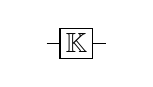
\begin{tikzpicture}[baseline={([yshift=-.5ex]current bounding box.center)}]
    \path (0,0) node (A) {}
    ++ (0.5,0) node[kernel] (K) {$\kernel{K}$}
    ++ (0.5,0) node (B) {};
    \draw (A) -- (K) -- (B);
\end{tikzpicture}\\
\mu&:= 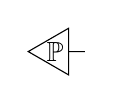
\begin{tikzpicture}[baseline={([yshift=-.5ex]current bounding box.center)}]
    \path (0,0) node[dist] (K) {$\kernel{P}$}
    ++ (0.5,0) node (B) {};
    \draw (K) -- (B);
\end{tikzpicture}
\end{align}

Given two Markov kernels $\kernel{L}:X\kto Y$ and $\kernel{M}:Y\kto Z$, the product $\kernel{L}\kernel{M}$ is represented by drawing them side by side and joining their wires:

\begin{align}
    \kernel{L}\kernel{M}:= 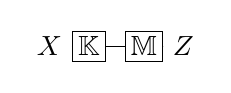
\begin{tikzpicture}[baseline={([yshift=-.5ex]current bounding box.center)}]
    \path (0,0) node (A) {$X$}
    ++ (0.5,0) node[kernel] (K) {$\kernel{K}$}
    ++ (0.7,0) node[kernel] (M) {$\kernel{M}$}
    ++ (0.5,0) node (B) {$Z$};
    \draw (A) -- (K) -- (M) -- (B);
\end{tikzpicture}
\end{align}

Given kernels $\kernel{K}:W\kto Y$ and $\kernel{L}:X\kto Z$, the tensor product $\kernel{K}\otimes\kernel{L}:W\times X\kto Y\times Z$ is graphically represented by drawing kernels in parallel:

\begin{align}
    \kernel{K}\otimes \kernel{L}&:=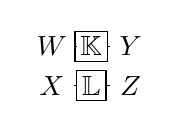
\begin{tikzpicture}[baseline={([yshift=-.5ex]current bounding box.center)}]
    \path (0,0) node (A) {$W$}
    ++ (0.5,0) node[kernel] (K) {$\kernel{K}$}
    ++ (0.5,0) node (B) {$Y$};
    \path (0,-0.5) node (C) {$X$}
    ++ (0.5,0) node[kernel] (L) {$\kernel{L}$}
    ++ (0.5,0) node (D) {$Z$};
    \draw (A) -- (K) -- (B);
    \draw (C) -- (L) -- (D);
\end{tikzpicture}
\end{align}

We read diagrams from left to right (this is somewhat different to \citet{fritz_synthetic_2020,cho_disintegration_2019,fong_causal_2013} but in line with \citet{selinger_survey_2011}), and any diagram describes a set of nested products and tensor products of Markov kernels. There are a collection of special Markov kernels for which we can replace the generic ``box'' of a Markov kernel with a diagrammatic elements that are visually suggestive of what these kernels accomplish.

The identity map $\text{id}_X:X\kto X$ defined by $(\text{id}_X)(A|x)= \delta_x(A)$ for all $x\in X$, $A\in\sigalg{X}$, is a bare line:

\begin{align}
    \mathrm{id}_X&:=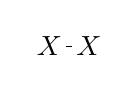
\begin{tikzpicture}[baseline={([yshift=-.5ex]current bounding box.center)}]
    \path (0,0) node (A) {$X$} ++ (0.5,0) node (B) {$X$};
    \draw (A) -- (B);
\end{tikzpicture}
\end{align}

Given some 1-element set $\{*\}$, the erase map $\text{del}_X:X\kto \{*\}$ defined by $(\text{del}_X)(*|x) = 1$ for all $x\in X$ is a Markov kernel that ``discards the input''. It looks like a lit fuse:

\begin{align}
    \text{del}_X&:=\begin{tikzpicture}[baseline={([yshift=-.5ex]current bounding box.center)}]
    \path (0,0) ++ (1,0) node (B) {$X$};
    \draw[-{Rays[n=8]}] (A) -- (B);
\end{tikzpicture}
\end{align}

The copy map $\text{copy}_X:X\kto X\times X$ defined by $(\text{copy}_X)(A\times B|x)=\delta_x(A)\delta_x(B)$ for all $x\in X$, $A,B\in \sigalg{X}$ is a Markov kernel that makes two identical copies of the input. It is drawn as a fork:

\begin{align}
    \text{copy}_X&:=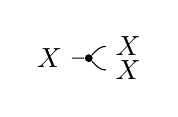
\begin{tikzpicture}[baseline={([yshift=-.5ex]current bounding box.center)}]
    \path (0,0) node (A) {$X$} 
    ++ (0.5,0) node[copymap] (copy0) {}
    ++ (0.5,0.15) node (B) {$X$}
    + (0,-0.3) node (C) {$X$};
    \draw (A) -- (copy0) to [out=45,in=180] (B) (copy0) to [out=-45, in=180] (C);
\end{tikzpicture}
\end{align}

The swap map $\text{swap}_{X,Y}:X\times Y\kto Y\times X$, defined by $(\text{swap}_{X,Y})(A\times B|x,y)=\delta_x(B)\delta_y(A)$ for $(x,y)\in X\times Y$, $A\in \sigalg{X}$ and $B\in \sigalg{Y}$, swaps two inputs and is represented by crossing wires:

\begin{align}
    \text{swap}_{X,Y} &:=  
\begin{tikzpicture}[baseline={([yshift=-.5ex]current bounding box.center)}]
        \path (0,0) node (A) {} 
        + (0,-0.5) node (B) {}
        ++ (1,0) node (C) {}
        + (0,-0.5) node (D) {};
        \draw (A) to [out=0,in=180] (D) (B) to [out=0, in=180] (C);
    \end{tikzpicture}
\end{align}

Diagrams in Markov categories satisfy the commutative comonoid axioms (see Definition \ref{def:mcat})

\begin{align}
    \tikzfig{ccom_lhs} = \tikzfig{ccom_rhs}\label{eq:ccom_1}
\end{align}
\begin{align}
    \tikzfig{ccom2_lhs} = \tikzfig{ccom2_mhs} = \tikzfig{ccom2_rhs}
\end{align}
\begin{align}
    \tikzfig{ccom3_lhs} = \tikzfig{ccom3_rhs}
\end{align}
as well as compatibility with the monoidal structure
\begin{align}
    \tikzfig{mstruct1_lhs} &= \tikzfig{mstruct1_rhs}\\
    \tikzfig{mstruct2_lhs} &= \tikzfig{mstruct2_rhs}
\end{align}
and the naturality of \emph{del}, which means that
\begin{align}
    \tikzfig{naturality_lhs} &= \tikzfig{naturality_rhs}\label{eq:nat}
\end{align}

\subsection{Iterated copy maps and plates}

The previous definitions are standard for Markov categories. We extend the graphical notation with $n$-fold maps and plates, which stand for tensor products repeated $n$ times.

\begin{definition}[$n$-fold copy map]
The $n$-fold copy map $\text{copy}^n_X:X\kto X^n$ is given by
\begin{align}
    \text{copy}^1_X &= \text{copy}_X\\
    \text{copy}^n_X &= \tikzfig{n_fold_copy} &n>1
\end{align}
\end{definition}

In a string diagram, a plate that is annotated $i\in A$ means the tensor product of the $|A|$ elements that appear inside the plate. A wire crossing from outside a plate boundary to the inside of a plate indicates an $|A|$-fold copy map, which we indicate by placing a dot on the plate boundary. We do not define anything that allows wires to cross from the inside of a plate to the outside; wires must terminate within the plate.

Thus, given $\kernel{K}_i:X\kto Y$ for $i\in A$,

\begin{align}
    \bigotimes_{i\in A} \kernel{K}_i &:= \tikzfig{plate_without_copymap}
    \text{copy}^{|A|}_X(\bigotimes_{i\in A} \kernel{K}_i) &:= \tikzfig{plate_with_copymap}
\end{align}


\subsubsection{Examples}
String diagrams can always be converted into definitions involving integrals and tensor products. A number of shortcuts can help to make the translations efficiently.

For arbitrary $\kernel{K}:X\times Y\kto Z$, $\kernel{L}:W\kto Y$

\begin{align}
    \tikzfig{identity_tensor_L} &= (\text{id}_X\otimes \kernel{L})\kernel{K}\\
    [(\text{id}_X\otimes \kernel{L})\kernel{K}](A|x,w) &= \int_{Y}\int_X   \kernel{K}(A|x',y')\kernel{L}(\mathrm{d}y'|w)\delta_x(\mathrm{d}x')\\
                                           &= \int_Y  \kernel{K}(A|x,y') \kernel{L}(dy'|w)
\end{align}

That is, an identity map ``passes its input directly to the next kernel''. 

For arbitrary $\kernel{K}: X\times Y\times Y\kto Z$:

\begin{align}
 \tikzfig{identity_tensor_copy} &= (\text{id}_X\otimes \text{copy}_Y)\kernel{K}\\
 [(\text{id}_X\otimes \text{copy}_Y)\kernel{K}](A|x,y) &= \int_Y\int_Y \kernel{K}(A|x,y',y'') \delta_y(\mathrm{d}y')\delta_y(\mathrm{d}y'')\\
                                           &= \kernel{K}(A|x,y,y)
\end{align}

That is, the copy map ``passes along two copies of its input'' to the next kernel in the product. 

For arbitrary $\kernel{K}:X\times Y\kto Z$

\begin{align}
    \tikzfig{swap_example} &= \text{swap}_{YX} \kernel{K}\\
    (\text{swap}_{YX}\kernel{K})(A|y,x) &= \int_{X\times Y} \kernel{K}(A|x',y')\delta_y(\mathrm{d}y')\delta_x(\mathrm{d}x')\\
                                        &= \kernel{K}(A|x,y)
\end{align}

The swap map before a kernel switches the input arguments.

For arbitrary $\kernel{K}:X\kto Y\times Z$

\begin{align}
    \tikzfig{swap_example_2} &= \kernel{K}\text{swap}_{YZ}\\
    (\kernel{K}\text{swap}_{YZ})(A\times B|x) &= \int_{Y\times Z} \delta_{y}(B)\delta_{z}(A)\kernel{K}(\mathrm{d}y\times\mathrm{d}z|x)\\
    &= \int_{B\times A} \kernel{K}(\mathrm{d}y\times\mathrm{d}z|x)\\
    &= \kernel{K}(B\times A|x)
\end{align}

\section{Probability sets}

A probability set is a set of probability measures. This section establishes a number of useful properties of conditional probability with respect to probability sets. Unlike conditional probability with respect to a probability space, conditional probabilities don't always exist for probability sets. Where they do, however, they are almost surely unique and we can marginalise and disintegrate them to obtain other conditional probabilities with respect to the same probability set.

\begin{definition}[Probability set]
A probability set $\prob{P}_{\{\}}$ on $(\Omega,\sigalg{F})$ is a collection of probability measures on $(\Omega,\sigalg{F})$. In other words it is a subset of $\mathscr{P}(\Delta(\Omega))$, where $\mathscr{P}$ indicates the power set.
\end{definition}

Given a probability set $\prob{P}_{\{\}}$, we define marginal and conditional probabilities as probability measures and Markov kernels that satisfy Definitions \ref{def:pushforward} and \ref{def:disint} respectively for \emph{all} base measures in $\prob{P}_{\{\}}$. There are generally multiple Markov kernels that satisfy the properties of a conditional probability with respect to a probability set, and this definition ensures that marginal and conditional probabilities are ``almost surely'' unique (Definition \ref{def:asequal}) with respect to probability sets.

\begin{definition}[Marginal probability with respect to a probability set]
Given a sample space $(\Omega,\sigalg{F})$, a variable $\RV{X}:\Omega\to X$ and a probability set $\prob{P}_{\{\}}$, the marginal distribution $\prob{P}_{\{\}}^{\RV{X}}=\prob{P}_\alpha^{\RV{X}}$ for any $\prob{P}_\alpha\in\prob{P}_{\{\}}$ if a distribution satisfying this condition exists. Otherwise, it is undefined.
\end{definition}

\begin{definition}[Uniform conditional distribution with respect to a probability set]\label{def:cprob_pset}
Given a sample space $(\Omega,\sigalg{F})$, variables $\RV{X}:\Omega\to X$ and $\RV{Y}:\Omega\to Y$ and a probability set $\prob{P}_{\{\}}$, a uniform conditional distribution $\prob{P}_{\{\}}^{\RV{Y}|\RV{X}}$ is any Markov kernel $X\kto Y$ such that $\prob{P}_{\{\}}^{\RV{Y}|\RV{X}}$ is an $\RV{Y}|\RV{X}$ conditional probability of $\prob{P}_\alpha$ for all $\prob{P}_\alpha\in \prob{P}_{\{\}}$. If no such Markov kernel exists, $\prob{P}_{\{\}}^{\RV{Y}|\RV{X}}$ is undefined.
\end{definition}

\begin{definition}[Uniform higher order conditional distribution with respect to a probability set]\label{def:ho_cprob_pset}
Given a sample space $(\Omega,\sigalg{F})$, variables $\RV{X}:\Omega\to X$, $\RV{Y}:\Omega\to Y$ and $\RV{Z}:\Omega\to Z$ and a probability set $\prob{P}_{\{\}}$, if $\prob{P}_{\{\}}^{\RV{ZY}|\RV{X}}$ exists then a uniform higher order conditional $\prob{P}_{\{\}}^{\RV{Z}|(\RV{Y}|\RV{X})}$ is any Markov kernel $X\times Y\kto Z$ that is a higher order conditional of some version of $\prob{P}_{\{\}}^{\RV{ZY}|\RV{X}}$. If no $\prob{P}_{\{\}}^{\RV{ZY}|\RV{X}}$ exists, $\prob{P}_{\{\}}^{\RV{Z}|(\RV{Y}|\RV{X})}$ is undefined.
\end{definition}

Under the assumption of standard measurable spaces, the existence of a uniform conditional distribution $\prob{P}_{\{\}}^{\RV{ZY}|\RV{X}}$ implies the existence of a higher order conditional $\prob{P}_{\{\}}^{\RV{Z}|(\RV{Y}|\RV{X})}$ with respect to the same probability set (Theorem \ref{th:ho_cond_psets}). $\prob{P}_{\{\}}^{\RV{Z}|(\RV{Y}|\RV{X})}$ is in turn a version of the uniform conditional distribution $\prob{P}_{\{\}}^{\RV{Z}|\RV{YX}}$ (Theorem \ref{th:higher_order_conditionals}). Thus, from the existence of $\prob{P}_{\{\}}^{\RV{ZY}|\RV{X}}$ we can derive the existence of $\prob{P}_{\{\}}^{\RV{Z}|\RV{YX}}$.

% \begin{lemma}[Equivalence of pushforward definitions]\label{lem:prod_pushf}
% Given a probability space $\kernel{M}:W\to \Omega$ and $\RV{X}:\Omega\to X$, define $\kernel{K}^{\RV{X}|\RV{W}}:W\kto X$ by $\kernel{K}^{\RV{X}|\RV{W}}(x|w):=\kernel{M}(\RV{X}\yields x|w)$ for any $x\in X$m $w\in W$ and $\kernel{L}^{\RV{X}}:W\kto X$ by
% \begin{align}
%   \kernel{L}^{\RV{X}|\RV{W}} = \kernel{M}\kernel{F}_{\RV{X}}
% \end{align}
% Then
% \begin{align}
% \kernel{L}^{\RV{X}|\RV{W}} =\kernel{K}^{\RV{X}|\RV{W}}
% \end{align}
% \end{lemma}

% \begin{proof}
% For any $x\in X$, $w\in W$
% \begin{align}
%   \kernel{L}^{\RV{X}|\RV{W}}(x|w) &= \sum_{\omega\in \Omega} \llbracket x=\RV{X}(\omega)\rrbracket \kernel{M}(\omega|w)\\
%                                   &= \sum_{\omega\in \RV{X}^{-1}(x)} \kernel{M}(\omega|w)\\
%                                   &= \kernel{M}(\RV{X}\yields x|w)\\
%                                   &= \kernel{K}^{\RV{X}|\RV{W}}(x|w)
% \end{align}
% \end{proof}

\subsection{Semidirect product and almost sure equality}

The operation used in Equation \ref{eq:conditional} that combines $\mu^{\RV{X}}$ and $\mu^{\RV{Y}|\RV{X}}$ is something we will use repeatedly, so we call it the \emph{semidirect product} and give it the symbol $\odot$. We also define a notion of almost sure equality with using $\odot$: $\kernel{K}\overset{\mu^{\RV{X}}}{\cong} \kernel{L}$ if $\mu^{\RV{X}}\odot \kernel{K}=\mu^{\RV{X}}\odot\kernel{L}$ (note that this latter equality is strict; both semidirect products must assign the same measure to the same measurable sets). Thus if two terms are almost surely equal, they are substitutable when they both appear in a semidirect product.

\begin{definition}[Semidirect product]\label{def:copyproduct}
Given $\prob{K}:X\kto Y$ and $\prob{L}:Y\times X\kto Z$, define the copy-product $\prob{K}\odot\prob{L}:X\to Y\times Z$ as
\begin{align}
    \prob{K}\odot\prob{L}:&= \text{copy}_X(\prob{K}\otimes \text{id}_X)(\text{copy}_Y\otimes\text{id}_X )(\text{id}_Y \otimes \prob{L})\\
                            &= \tikzfig{copy_product}\\
                            &\iff\\
    (\prob{K}\odot\prob{L})(A\times B|x) &= \int_A \prob{L}(B|y,x)\prob{K}(dy|x)&A\in \sigalg{Y},B\in\sigalg{Z}
\end{align}
\end{definition}

\begin{lemma}[Semidirect product is associative]
Given $\prob{K}:X\kto Y$, $\prob{L}:Y\times X\kto Z$ and $\prob{M}:Z\times Y\times X\kto W$
\begin{align}
    (\prob{K}\odot \prob{L})\odot \prob{Z} &= \prob{K}\odot(\prob{L}\odot\prob{Z})\\
\end{align}
\end{lemma}

\begin{proof}
\begin{align}
    (\prob{K}\odot \prob{L})\odot \prob{M} &= \tikzfig{odot_assoc_1}\\
                                            &=  \tikzfig{odot_assoc_2}\\
                                            &= \prob{K}\odot (\prob{L}\odot \prob{M})
\end{align}
\end{proof}

Two Markov kernels are almost surely equal with respect to a probability set $\prob{P}_{\{\}}$ if the semidirect product $\odot$ of all marginal probabilities of $\prob{P}_\alpha^\RV{X}$ with each Markov kernel is identical.

\begin{definition}[Almost sure equality]\label{def:asequal}
Two Markov kernels $\kernel{K}:X\kto Y$ and $\kernel{L}:X\kto Y$ are almost surely equal $\overset{\prob{P}_{\{\}}}{\cong}$ with respect to a probability set $\prob{P}_{\{\}}$ and variable $\RV{X}:\Omega\to X$ if for all $\prob{P}_\alpha \in \prob{P}_{\{\}}$,
\begin{align}
    \prob{P}^{\RV{X}}_\alpha\odot \kernel{K}=\prob{P}^{\RV{X}}_\alpha\odot \kernel{L}
\end{align}
\end{definition}

\begin{lemma}[Uniform conditional distributions are almost surely equal]
If $\kernel{K}:X\kto Y$ and $\kernel{L}:X\kto Y$ are both versions of $\prob{P}_{\{\}}^{\RV{Y}|\RV{X}}$ then $\kernel{K}\overset{\prob{P}_{\{\}}}{\cong}\kernel{L}$
\end{lemma}

\begin{proof}
For all $\prob{P}_\alpha \in \prob{P}_{\{\}}$
\begin{align}
    \prob{P}^{\RV{X}}_\alpha\odot \kernel{K} &= \prob{P}^{\RV{XY}}_\alpha\\
    &= \prob{P}^{\RV{X}}_\alpha\odot \kernel{L}
\end{align}
\end{proof}

\begin{lemma}[Substitution of almost surely equal Markov kernels]\label{lem:sub_asequal}
Given $\prob{P}_{\{\}}$, if $\kernel{K}:X\times Y \kto Z$ and $\kernel{L}:X\times Y \kto Z$ are almost surely equal $\kernel{K}\overset{\prob{P}_{\{\}}}{\cong}\kernel{L}$, then for any $\prob{P}_\alpha\in \prob{P}_{\{\}}$
\begin{align}
    \prob{P}_\alpha^{\RV{Y}|\RV{X}}\odot \kernel{K} &\overset{\prob{P}_{\{\}}}{\cong} \prob{P}_\alpha^{\RV{Y}|\RV{X}}\odot \kernel{L}
\end{align}
\end{lemma}

\begin{proof}
For any $\prob{P}_\alpha\in\prob{P}_{\{\}}$
\begin{align}
    \prob{P}_\alpha^{\RV{XY}}\odot \kernel{K} &= (\prob{P}_\alpha^{\RV{X}}\odot \prob{P}_{\{\}}^{\RV{Y}|\RV{X}})\odot \kernel{K}\\
                                              &= \prob{P}_\alpha^{\RV{X}}\odot (\prob{P}_{\{\}}^{\RV{Y}|\RV{X}}\odot \kernel{K})\\
                                              &= \prob{P}_\alpha^{\RV{X}}\odot (\prob{P}_{\{\}}^{\RV{Y}|\RV{X}}\odot \kernel{L})
\end{align}
\end{proof}

\begin{theorem}[Semidirect product of uniform conditional distributions is a joint uniform conditional distribution]\label{lem:joint_conditional}
Given a probability set $\prob{P}_{\{\}}$ on $(\Omega,\sigalg{F})$, variables $\RV{X}:\Omega\to X$, $\RV{Y}:\Omega\to Y$ and uniform conditional distributions $\prob{P}_{\{\}}^{\RV{Y}|\RV{X}}$ and $\prob{P}_{\{\}}^{\RV{Z}|\RV{XY}}$, then $\prob{P}_{\{\}}^{\RV{YZ}|\RV{X}}$ exists and is equal to
\begin{align}
    \prob{P}_{\{\}}^{\RV{YZ}|\RV{X}} &= \prob{P}_{\{\}}^{\RV{Y}|\RV{X}}\odot \prob{P}_{\{\}}^{\RV{Z}|\RV{XY}}
\end{align}
\end{theorem}

\begin{proof}
By definition, for any $\prob{P}_\alpha\in \prob{P}_{\{\}}$
\begin{align}
    \prob{P}_\alpha^{\RV{XYZ}} &= \prob{P}_\alpha^{\RV{X}}\odot \prob{P}_\alpha^{\RV{YZ}|\RV{X}}\\
                               &= \prob{P}_\alpha^{\RV{X}}\odot(\prob{P}_\alpha^{\RV{Y}|\RV{X}}\odot \prob{P}_\alpha^{\RV{Z}|\RV{YX}})\\
                               &= \prob{P}_\alpha^{\RV{X}}\odot(\prob{P}_{\{\}}^{\RV{Y}|\RV{X}}\odot \prob{P}_{\{\}}^{\RV{Z}|\RV{YX}})
\end{align}
\end{proof}

\subsection{Conditional independence}

Conditional independence has a familiar definition in probability models. It is sometimes possible to infer the existence of a uniform conditional probability from a conditional independence statement. Conditional independence can be equivalently defined either in terms of a factorisation of a joint probability distribution (Definition \ref{def:ci}) or in terms of the existence of a conditional distribution that ignores one of its inputs (Theorem \ref{th:cho_ci_equiv}). 

The latter formulation allows us, in some cases, to conclude from a the combination of a uniform conditional probability and a conditional independence statement the existence of a further uniform conditional probability (Corollary \ref{cor:ci_cp_exist}). We will discuss in Section \ref{sec:dec_probs} how uniform conditional probabilities can be thought of as causal relationships. Thus this means: from a fundamental assumed causal relationship and a conditional independence observed under the right conditions, we can conclude the existence of an additional causal relationship. 

\begin{definition}[Conditional independence]\label{def:ci}
For a \emph{probability model} $\model{P}_{\alpha}$ and variables $\RV{A},\RV{B},\RV{Z}$, we say $\RV{B}$ is conditionally independent of $\RV{A}$ given $\RV{C}$, written $\RV{B}\CI_{\model{P}_{\alpha}}\RV{A}|\RV{C}$, if
\begin{align}
    \kernel{P}_{\alpha}^{\RV{ABC}} &= \tikzfig{cond_indep1} \label{eq:cond_indep}
\end{align}
\end{definition}

\citet{cho_disintegration_2019} have shown that this definition coincides with the standard notion of conditional independence for a particular probability model (Theorem \ref{th:cho_ci_equiv}). 

Conditional independence can equivalently be stated in terms of the existence of a conditional probability that ``ignores'' one of its inputs.

\begin{theorem}\label{th:cho_ci_equiv}
Given standard measurable $(\Omega,\sigalg{F})$, a probability model $\prob{P}$ and variables $\RV{W}:\Omega\to W$, $\RV{X}:\Omega\to X$, $\RV{Y}:\Omega\to Y$, $\RV{Y}\CI_{\prob{P}}\RV{X}|\RV{W}$ if and only if there exists some version of $\prob{P}^{\RV{Y}|\RV{WX}}$ and $\kernel{K}:W\kto Y$ such that
\begin{align}
    \prob{P}^{\RV{Y}|\RV{WX}} &= \tikzfig{cond_indep_erase}\\
    \iff
    \prob{P}^{\RV{Y}|\RV{WX}}(A|w,x) &= \prob{K}(A|w)&\forall A\in \sigalg{Y}
\end{align}
\end{theorem}

\begin{proof}
See \citet{cho_disintegration_2019}.
\end{proof}

Theorem \ref{th:cons_ci} shows how, under some circumstances, it is possible to infer an extended conditional independence in a probability set $\prob{P}_C$ from a regular conditional independence that holds in one element of the set $\prob{P}_\alpha$. We ultimately carry out the procedure associated with on only one element of $C$, so usually we cannot test whether some property holds for the whole set $\prob{P}_C$. However, regular conditional independences with respect to a particular element of $\prob{P}_C$ can be tested for (again, subject to some assumptions \citep{shah_hardness_2020}).

\begin{theorem}\label{th:cons_ci}
Given standard measurable $(\Omega,\sigalg{F})$, variables $\RV{W}:\Omega\to W$, $\RV{X}:\Omega\to X$, $\RV{Y}:\Omega\to Y$ and a probability set $\prob{P}_{C}$ with uniform conditional probability $\prob{P}_{C}^{\RV{Y}|\RV{WX}}$ and $\alpha\in C$ such that $\prob{P}_\alpha^{\RV{WX}}\gg \{\prob{P}_\beta^{\RV{WX}}|\beta\in C\}$, $\RV{Y}\CI_{\prob{P}_{\alpha}}\RV{X}|\RV{W}$ if and only if there is a version of $\prob{P}_{C}^{\RV{Y}|\RV{WX}}$ and $\kernel{K}:W\kto Y$ such that
\begin{align}
  \prob{P}_C^{\RV{Y}|\RV{WX}} &= \tikzfig{cond_indep_erase} \label{eq:higherorder_ci_erase}
\end{align}
\end{theorem}

\begin{proof}
See Appendix \ref{sec:cond_ind_app}
\end{proof}

\begin{corollary}\label{cor:ci_cp_exist}
Given standard measurable $(\Omega,\sigalg{F})$, variables $\RV{W}:\Omega\to W$, $\RV{X}:\Omega\to X$, $\RV{Y}:\Omega\to Y$ and a probability set $\prob{P}_{C}$ with uniform conditional $\prob{P}_{C}^{\RV{Y}|\RV{WX}}$ and $\alpha\in C$ such that $\prob{P}_\alpha^{\RV{WX}}\gg \{\prob{P}_\beta^{\RV{WX}}|\beta\in C\}$, $\prob{P}_{C}^{\RV{Y}|\RV{W}}$ exists if $\RV{Y}\CI_{\prob{P}_{\alpha}}\RV{X}|\RV{W}$.
\end{corollary}

\begin{proof}
By Theorem \ref{th:cons_ci}, there is $\kernel{K}:W\kto Y$ such that for all $\beta$
\begin{align}
    \prob{P}_{\beta}^{\RV{WY}} &= \tikzfig{conditional_independence_cprob_exist}\\
    &= \tikzfig{conditional_independence_cprob_exist2}\\
    &= \tikzfig{conditional_independence_cprob_exist3}
\end{align}

Thus $\kernel{K}$ is a version of $\prob{P}_{C}^{\RV{Y}|\RV{W}}$.
\end{proof}

\subsection{Uniform conditional independence}\label{sec:eci}

There are different notions of conditional independence that could be applied to a probability set $\prob{P}_C$. We can say $\RV{X}$ is ``globally independent'' of $\RV{Y}$ given $\RV{Z}$ if for every $\prob{P}_\alpha\in \prob{P}_C$, $\RV{X}\CI_{\prob{P}_\alpha}\RV{Y}|\RV{Z}$. Alternatively, we can say $\RV{X}$ is ``uniformly independent'' of $\RV{Y}$ given $\RV{Z}$ if $\prob{P}_C^{\RV{X}|\RV{YZ}}$ exists and does not depend on $\RV{Y}$. We are particularly interested in the second kind, as this is the kind of conditional independence that enables simplified representations of uniform conditional distributions.

Both of these kinds of conditional independence are special cases of \emph{extended conditional independence}, introduced by \citet{constantinou_extended_2017}. Extended conditional independence is a generalisation of conditional independence that is applicable to probability sets. In full generality, extended conditional independence makes use of the notion of ``nonstochastic variables'', which are analogous to our notion of observed variables but applied to the set of choices $C$.

Extended conditional independence provides a unified way to express global conditional independence, uniform conditional independence and forms of conditional independence intermediate between the two. However, we only make use of uniform conditional independence in this work.

\begin{definition}[Uniform conditional independence]\label{def:eci}
Given a probability set $\prob{P}_C$ and variables $\RV{X}$, $\RV{Y}$ and $\RV{Z}$, the uniform conditional independence $\RV{Y}\CI^e_{\prob{P}_C} \RV{X} C|\RV{Z}$ holds if $\prob{P}_C^{\RV{Y}|\RV{XZ}}$ and $\prob{P}_C^{\RV{Y}|\RV{X}}$ exist and
\begin{align}
    \prob{P}_C^{\RV{Y}|\RV{XZ}} &\overset{\prob{P}_C}{\cong} \tikzfig{eci_def}\\
    &\iff\\
    \prob{P}_C^{\RV{Y}|\RV{XZ}}(A|x,z) &\overset{\prob{P}_C}{\cong} \prob{P}_C^{\RV{Y}|\RV{Z}}(A|z)&\forall A\in \sigalg{Y},(x,z)\in X\times Z\label{eq:eci}
\end{align}
\end{definition}

The notation $\RV{Y}\CI^e_{\prob{P}_C} \RV{X} C|\RV{Z}$ is intentionally similar to a statement of extended conditional independence as defined by \citet{constantinou_extended_2017}. However, uniform conditional independence is a stronger assumption than extended conditional independence as the latter allows for arbitrary functions satisfy an equation like Eq. \ref{eq:eci}, while we require that these functions are Markov kernels (the are measurable and probability distribution-value, as in Definition \ref{def:mkern}).

\begin{example}[Choice variable]\label{ex:choice_var}
Suppose we have a decision procedure $\proc{S}_C:=\{\proc{S}_\alpha|\alpha\in C\}$ that consists of a measurement procedure for each element of a denumerable set of choices $C$. Each measurement procedure $\proc{S}_\alpha$ is modeled by a probability distribution $\prob{P}_\alpha$ on a shared sample space $(\Omega,\sigalg{F})$ such that we have an observable ``choice'' variable $(\RV{D},\RV{D}\circ\proc{S}_\alpha)$ where $\RV{D}\circ\proc{S}_\alpha$ always yields $\alpha$.

Furthermore, Define $\RV{Y}:\Omega\to \Omega$ as the identity function. Then, by supposition, for each $\alpha\in A$, $\prob{P}_\alpha^{\RV{Y}\RV{C}}$ exists and for $A\in \sigalg{Y}$, $B\in \sigalg{C}$:

\begin{align}
    \prob{P}_\alpha^{\RV{YC}}(A\times B) &= \prob{P}_\alpha(A)\delta_\alpha(B)
\end{align}

This implies, for all $\alpha\in C$

\begin{align}
    \prob{P}_\alpha^{\RV{Y}|\RV{D}} &= \prob{P}_\alpha^{\RV{Y}}
\end{align}

Thus $\prob{P}_C^{\RV{Y}|\RV{D}}$ exists and

\begin{align}
    \prob{P}_C^{\RV{Y}|\RV{D}}(A|\alpha) &= \prob{P}_\alpha^{\RV{Y}} (A)&\forall A\in \sigalg{Y},\alpha\in C 
\end{align}

Because only deterministic marginals $\prob{P}_\alpha^{\RV{D}}$ are available, for every $\alpha\in C$ we have $\RV{Y}\CI_{\prob{P}_\alpha} \RV{D}$. This reflects the fact that \emph{after we have selected a choice $\alpha$} the value of $\RV{C}$ provides no further information about the distribution of $\RV{Y}$, because $\RV{D}$ is deterministic given any $\alpha$. It does not reflect the fact that ``choosing different values of $\RV{C}$ has no effect on $\RV{Y}$''.
\end{example}

\begin{theorem}[Uniform conditional independence representation]\label{th:uci_rep}
Given a probability set $\prob{P}_C$ with a uniform conditional probability $\prob{P}^{\RV{XY}|\RV{Z}}_C$,
\begin{align}
    \prob{P}^{\RV{XY}|\RV{Z}}_C &\overset{\prob{P}_C}{\cong} \tikzfig{eci_rep}\\
    &\iff\\
    \prob{P}^{\RV{XY}|\RV{Z}}_C(A\times B|z) &\overset{\prob{P}_C}{\cong} \prob{P}_C^{\RV{X}|\RV{Z}}(A|z)\prob{P}_C^{\RV{Y}|\RV{Z}}(B|z)&\forall A\in \sigalg{X},B\in \sigalg{Y},z\in Z
\end{align}
if and only if $\RV{Y}\CI_{\prob{P}_C}^e \RV{X}C|\RV{Z}$
\end{theorem}

\begin{proof}
If:
By Theorem \ref{th:higher_order_conditionals}
\begin{align}
    \prob{P}^{\RV{XY}|\RV{Z}}_C &= \tikzfig{eci_rep_1}\\
    &\overset{\prob{P}_C}{\cong} \tikzfig{eci_rep_2}\\
    &= \tikzfig{eci_rep}
\end{align}
Only if:
Suppose
\begin{align}
    \prob{P}^{\RV{XY}|\RV{Z}}_C &\overset{\prob{P}_C}{\cong} \tikzfig{eci_rep}
\end{align}
and suppose for some $\alpha\in C$, $A\times C\in \sigalg{X}\otimes\sigalg{Z}$, $B\in \sigalg{Y}$ $\prob{P}_\alpha^{\RV{XZ}}(A\times C)>0$ and
\begin{align}
    \prob{P}_C^{\RV{Y}|\RV{XZ}}(B|x,z) &> \prob{P}_C^{\RV{Y}|\RV{Z}}(B|z)& \forall (x,z)\in A\times C \label{eq:assume_ieq}
\end{align}
then
\begin{align}
    \prob{P}_\alpha^{\RV{XYZ}\RV{Z}}(A\times B\times C) &= \int_{A\times C} \prob{P}_C^{\RV{Y}|\RV{XZ}}(B|x,z)\prob{P}_C^{\RV{X}|\RV{Z}}(\mathrm{dx}|z)\prob{P}_\alpha^{\RV{Z}}(\mathrm{dz})\\
    &> \int_{A\times C} \prob{P}_C^{\RV{Y}|\RV{X}}(B|z)\prob{P}_C^{\RV{X}|\RV{Z}}(\mathrm{dx}|z)\prob{P}_\alpha^{\RV{Z}}(\mathrm{dz})\\
    &= \int_{C} \prob{P}_C^{\RV{XY}|\RV{X}}(A\times B|z)\prob{P}_\alpha^{\RV{Z}}(\mathrm{dz})\\
    &= \prob{P}_\alpha^{\RV{XYZ}\RV{Z}}(A\times B\times C)
\end{align}
a contradiction. An analogous argument follows if we replace ``$>$'' with ``$<$'' in Eq. \ref{eq:assume_ieq}.
\end{proof}

% \begin{theorem}[Disintegrations are conditional probabilities]
% Suppose we have a fundamental probability set $\Omega$ variables $\RV{W}:\Omega\to W$, $\RV{X}:\Omega\to X$, $\RV{Y}:\Omega\to Y$ and $\RV{Z}:\Omega\to Z$ and a probability set $\prob{P}_{\{\}}$ such that $\prob{P}_{\{\}}^{\RV{X}|\RV{Y}}$ is a $\RV{Y}|\RV{X}$ conditional probability and there is some $\kernel{K}^{\RV{$
% \end{theorem}

% Given a conditional probability with respect to a probability gap model, we can also find additional conditional probabilities by disintegrating the original conditional probability.

% \begin{lemma}[Recursive disintegration]
% Suppose we have a fundamental probability set $\Omega$, variables $\RV{W}:\Omega\to W$, $\RV{X}:\Omega\to X$ and $\RV{Y}:\Omega\to Y$, $\RV{Z}:\Omega\to Z$ and a probability set $\prob{P}_{\{\}}$ such that $\prob{P}_{\{\}}^{\RV{X}|\RV{Y}}$ is a $\RV{Y}|\RV{X}$ conditional probability. Define $\prob{Q}_{\{\}}$ as the largest probability set such that $\prob{Q}_{\{\}}^{\RV{Y}|\RV{X}}=\prob{P}_{\{\}}^{\RV{Y}|\RV{X}}$. Then if $\prob{Q}_{\{\}}^{\RV{Z}|\RV{W}}$ is a $\RV{Z}|\RV{W}$ conditional probability of $\prob{Q}_{\{\}}$, it is also a $\RV{Z}|\RV{W}$ conditional probability of $\prob{P}_{\{\}}$.
% \end{lemma}

% \begin{proof}
% $\prob{Q}_{\{\}}\supset \prob{P}_{\{\}}$, so any conditional probability of $\prob{Q}_{\{\}}$ is also a conditional probability of $\prob{P}_{\{\}}$.
% \end{proof}



% \begin{definition}[Conditional independence with respect to a probability comb]
% Conditional independence $\RV{A}\CI_{\prob{P}_\square}\RV{B}|\RV{C}$ holds for an arbitrary probability comb $\model{P}_\square:A\to \mathscr{P}(\Delta(\Omega))$ if $\RV{A}\CI_{\prob{P}_\alpha}\RV{B}|\RV{C}$ holds for all probability models $\prob{P}_\alpha$, $\alpha\in A$.
% \end{definition}

%!TEX root = main.tex



\section{Syntax and semantics of causal consequences}

Causal Bayesian networks and potential outcomes employ different naming conventions to distinguish ``causal effects'' from ``simple correlations''. Causal Bayesian networks write $P(\RV{Y}|do(\RV{X}))$ and $P(\RV{Y}|\RV{X})$, while potential outcomes distinguishes $P(\RV{Y}|\RV{X})$ from $x\mapsto P(\RV{Y}^x)$. If we are not going to worry too much about details of interpretation, we can interpret the expression $P(\RV{Y}|\RV{X})$ as expressing something like this: there is an objective probability $P(\RV{Y},\RV{X})$ that describes a sequence of independent and identically distributed observations, and $P(\RV{Y}|\RV{X})$ is a disintegration of this probability. The existence of an objective probability $P(\RV{Y},\RV{X})$ can be justified by an assumption that the sequence of observations should be modeled exchangeably.

We pursue a similar line of thinking with respect to understanding causal consequences like $P(\RV{Y}|do(\RV{X}))$ or $x\mapsto P(\RV{Y}^x)$. We assume that ``causal consequences'' are conditional probabilities of the form $\prob{P}_\square^{\RV{Y}|\RV{D}\RV{H}}$ where $\RV{Y}$ is an outcome, $\RV{D}$ is some decision, $\RV{H}$ is a hypothesis and $\prob{P}_\square$ is a probability gap model. Our interest is in understanding what causal consequences are \emph{from the point of view of someone choosing a decision function}. We do not address the question of how they may be inferred from observed data.

 We show that conditional probability models that are \emph{causally contractible} with respect to a sequence of decisions and a corresponding sequence of outcomes are representible by mixtures of ``objective but unknown'' conditional probabilities. This is analogous to De Finetti's theorem that shows exchangeable probability distributions are representable by mixtures of ``objective but unknown'' independent and identically distributed probability distributions. A similar argument to ours is found in \citet{dawid_decision-theoretic_2020}.

We also consider the question of when causal contractibility could be supposed to hold. This is a subtle question, as the answer appears to differ for situations that are quite similar. For example, consider:
\begin{enumerate}
    \item Dr Alice is going to see two patients who are both complaining of lower back pain and are otherwise unknown to Alice. Prior to seeing them, she considers the available research and formulates a general sense of whether or not she'll treat each one, which she quantifies with $\prob{P}_\alpha^{\RV{D}_1\RV{D}_2}$
    \item As before, but prior to seeing the patients she considers the available research and decides to treat on the basis of applying a function to a random number generator with known characteristics. The choice of function and random number generator allow her to quantity probability of treatment with $\prob{P}_\alpha^{\RV{D}_1\RV{D}_2}$
\end{enumerate}

\todo[inline]{I removed the discussion of probability combs for simplicity, so I have not considered policies for treatment that depend on earlier experiments in the examples above}

We will argue that Alice could reasonably assume causal contractibility in the second case but not the first. While we are unable to offer a general theory of when causal contractibility holds, we note that an apparently key difference between the two situations is that in the first case the ``decision'' $\RV{D}_1$ is indeterministic for some $\alpha$, though $\RV{D}_2$ is deterministic, while in the second case both $\RV{D}_1$ and $\RV{D}_2$ are determinstic functions.

\subsection{Repeatable experiments}

A conditional probability model $(\prob{P}_\square^{\overline{\RV{Y}|\RV{D}}},A)$ is a model of a sequential experiment if $\RV{Y}:=\RV{Y}_M=(\RV{Y}_i)_{i\in M}$ and $\RV{D}:=\RV{D}_M=(\RV{D}_i)_{i\in M}$ for some index set $M$. We say that $\RV{Y}_i$ is the consequence corresponding to the decision $\RV{D}_i$ for all $i\in M$. We identify a ``causal consequence'' with a conditional probability of the form $\prob{P}_\square^{\RV{Y}_i|\RV{H}\RV{D}_i}$, where $\RV{H}$ is a hypothesis that is deterministically identical for every $i$. Causal consequences do not generally exist, see Definition \ref{def:cprob_pset}.

If $(\prob{P}_\square^{\overline{\RV{Y}|\RV{D}}},A)$ represents a sequential experiment, we might guess that causal consequences exist if the experiment is in some sense ``repeatable''. We consider two precise notions of repeatability. The first condition is \emph{commutativity of exchange}, which is the assumption that swapping the choices that we apply at each step and then applying the corresponding inverse swap to consequences leaves the model unchanged. The second condition is \emph{commutativity of marginalisation} -- if we perform the whole experiment multiple times, making the same choice $\RV{D}_i$ at any point $i$ gets the same results, regardless of what other choices are made.

Commutativity of exchange is similar to the condition of \emph{post-treatment exchangeability} found in \citet{dawid_decision-theoretic_2020}, and commutativity of marginalisation is similar to the stable unit treatment distribution assumption (SUTDA) in the same, as well as the ``no interference'' part of the stable unit treatment value assumption (SUTVA) with which it shares a name. Commutativity of exchange is also very similar to the exchangeability assumption of \citet{greenland_identifiability_1986} for further discussions of exchangeability in the context of causal modelling, and note that both authors consider exchanging to be an operation that alters which person receives which treatment. The assumption of exchangeability found in \citet{banerjee_chapter_2017} can also be regarded as similar to commutativity of exchange.

\todo[inline]{Not sure if or where I want to put this, I just think it helps to illustrate the difference}

Commutativity of exchange is not equivalent to exchangeability in the sense of De Finetti's well-known theorem \citet{de_finetti_foresight_1992}. The latter can be understood as expressing an indifference between conducting the experiment as normal, or conducting the experiment and then swapping some labels. However, swapping \emph{choices} will (usually) lead to different ``pieces of the experiment'' receiving different treatment, which is something that can't be achieved by swapping labels after the experiment has concluded.

The difference is illustrated by the following pair of diagrams.

Exchangeability (swapping labels):

\begin{align}
    \tikzfig{exchangeability}
\end{align}

Commutativity of exchange (swapping choices $\sim$ swapping labels):

\begin{align}
    \tikzfig{commutativity of exchange}
\end{align}

Commutativity of exchange is a property of probability gap models, not a property of fixed probability model for which there is no analogue of ``attaching a different choice'' in that case.

\todo[inline]{----end not sure where to put------}


% Another way to see where we are going is to consider graphical statements of our and De Finetti's result.

% Take $S=\{0,1\}$ and identify the space $\Delta(S)$ of probability measures on $S$ with the interval $[0,1]$. De Finetti showed that any infinite exchangeable probability measure $\prob{P}_\alpha$ on $\{0,1\}^\mathbb{N}$ can be represented by a prior $\prob{P}_\alpha^{\RV{H}}\in [0,1]$ for some $\RV{H}:\Omega\to H$ and a conditional probability $\prob{P}^{\RV{S}_0|\RV{H}}:[0,1]\kto \{0,1\}$ such that

% \begin{align}
%     \prob{P}_\alpha &= \tikzfig{de_finetti_rep0}\label{eq:definettirep}
% \end{align}

% Here $\prob{P}^{\RV{S}_0|\RV{H}}$ can be defined concretely by $\prob{P}^{\RV{S}_0|\RV{H}}(1|h)=h$. Equivalently, the probability gap model on $S^\mathbb{N}$ defined by the assumption of exchangeability is equivalent to the probability gap model defined by the conditional probability

% \begin{align}
%     \prob{P}^{\RV{S}|\RV{H}} = \tikzfig{de_finetti_conditional}
% \end{align}

% That is, there is some hypothesis $\RV{H}$ and conditional on $\RV{H}$ the measurements are independent and identically distributed. The proof of this is constructive -- $\RV{H}$ is a function of $\RV{S}$.



% \begin{align}
%     \prob{P}^{\RV{Y}|\RV{HD}} = \tikzfig{do_model_representation}
% \end{align}

% We will further argue that the class of see-do models considered in CBN and potential outcomes literature is equivalent to the family of causally contractible and exchangeable do-models where the decision rule for the first $n$ places is fixed to an unknown value, and may be freely chosen thereafter.

% \begin{theorem}[Existence of conditional in do models]
% Given a do model $(\prob{P}_{\square}^{\RV{Y}\|\RV{D}},R)$, for all $\alpha\in R$, $n\in\mathbb{N}$
% \begin{align}
%     \prob{P}_\alpha^{\RV{Y}_{[n]}\RV{D}_i} = \prob{P}_\alpha^{\RV{D}_{[n]}}\odot \prob{P}_\square^{\RV{Y}_{[n]}\|\RV{D}_{[n]}}
% \end{align}
% That is, $\prob{P}_\square^{\RV{Y}_{[n]}\|\RV{D}_{[n]}}\cong \prob{P}_\square^{\RV{Y}_{[n]}|\RV{D}_{[n]}}$
% \end{theorem}

% \begin{proof}
% For any $n>1\in \mathbb{N}$, $\alpha\in R$

% \begin{align}
%     \prob{P}_\alpha^{\RV{Y}_{[n]}\RV{D}_{[n]}} &= \tikzfig{do_model_1}\\
%     &= \tikzfig{do_model_2}\\
%     &= \tikzfig{do_model_3}\\
%     &= \tikzfig{do_model_4}\\
%     \implies \prob{P}_\alpha^{\RV{Y}_{[n]}|\RV{D}_{[n]}} &= \tikzfig{do_model_5}\\
%     &= \prob{P}_\alpha^{\RV{Y}_{[n-1]}|\RV{D}_{[n-1]}}\combprod \prob{P}_\square^{\RV{Y}_n|\RV{Y}_{[n-1]}\RV{D}_n}
% \end{align}

% Applying this recursively with $\prob{P}_\alpha^{\RV{Y}_{[1]}|\RV{D}_{[1]}}=\prob{P}_\square^{\RV{Y}_{[1]}|\RV{D}_{[1]}}$ yields

% \begin{align}
%     \prob{P}_\alpha^{\RV{Y}_{[n]}|\RV{D}_{[n]}} = \prob{P}_\square^{\RV{Y}_{[n]}\|\RV{D}_{[n]}}
% \end{align}
% as desired.
% \end{proof}
More precisely, a conditional probability model ``commutes with exchange'' if applying any finite permutation to blind choices or separately applying the corresponding permuation to consequences each yields the same result. We can apply the exchange ``before'' multiplying by the conditional $\prob{P}_{\square}^{\RV{Y}|\RV{D}}$ or after it and we get the same result.

\begin{definition}[Swap map]
Given $M\subset \mathbb{N}$ a finite permutation $\rho:M\to M$ and a variable $\RV{X}:\Omega\to X^M$ such that $\RV{X}=(\RV{X}_i)_{i\in M}$, define the Markov kernel $\text{swap}_{\rho(\RV{X})}:X^M\kto X^M$ by $(d_i)_{i\in\mathbb{N}}\mapsto \delta_{(d_{\rho(i)})_{i\in\mathbb{N}}}$.
\end{definition}

\begin{definition}[Commutativity of exchange]\label{def:caus_exch}
Suppose we have a sample space $(\Omega,\sigalg{F})$ and a conditional probability model $(\prob{P}_{\square}^{\overline{\RV{Y}|\RV{D}}},A)$ with $\RV{Y}=\RV{Y}_M$, $\RV{D}=\RV{D}_M$, $M\subseteq \mathbb{N}$. If, for any two decision rules $\alpha^{\overline{\RV{D}}},\beta^{\overline{\RV{D}}} \in A$,
\begin{align}
    \alpha^{\RV{D}}\odot \text{swap}_{\rho(\RV{D})} \prob{P}_{\square}^{\RV{Y}|\RV{D}} &= \alpha^{\RV{D}}\odot \prob{P}_{\square}^{\RV{Y}|\RV{D}}\text{swap}_{\rho(\RV{Y})}
\end{align}
Then $\prob{P}_\square$ \emph{commutes with exchanges}.
\end{definition}

A do model is non interfering if it gives identical results for identical subsequences of different choices when we limit our attention to the corresponding subsequences of consequences. For example, if we have $\RV{D}=(\RV{D}_1,\RV{D}_2,\RV{D}_3)$ and $\RV{Y}=(\RV{Y}_1,\RV{Y}_2,\RV{Y}_3)$ and $\alpha^{\RV{D}_1\RV{D}_3}=\prob{P}_\beta^{\RV{D}_1\RV{D}_3}$ then $\prob{P}_{\alpha}^{\RV{Y}_1\RV{D}_1\RV{Y}_3\RV{D}_3}=\prob{P}_\beta^{\RV{Y}_1\RV{D}_1\RV{Y}_3\RV{D}_3}$.

\begin{definition}[Commutativity of marginalisation]\label{def:caus_cont}
Suppose we have a sample space $(\Omega,\sigalg{F})$ and a conditional probability model $(\prob{P}_{\square}^{\overline{\RV{Y}|\RV{D}}},A)$ with $\RV{Y}=\RV{Y}_M$, $\RV{D}=\RV{D}_M$, $M\subseteq \mathbb{N}$. For any $S=(s_i)_{i\in Q}$, $Q\subset M$, and $i<j\implies p_i<p_j \And q_i<q_j$, let $\RV{D}_S:=(\RV{D}_i)_{i\in S}$ and $\RV{D}_T:=(\RV{D}_i)_{i\in T}$. If for any $\alpha,\beta\in R$
\begin{align}
    \prob{P}_\alpha^{\RV{D}_{S}}&=\prob{P}_\beta^{\RV{D}_{S}}\\
    \implies \prob{P}_\alpha^{(\RV{D_i,Y_i})_{i\in S}}&=\prob{P}_\beta^{(\RV{D_i,Y_i})_{i\in S}}
\end{align}
then $\prob{P}_\square$ \emph{commutes with marginalisation}.
\end{definition}

Neither condition implies the other. 
\begin{lemma}
Commutativity of exchange does not imply commutativity or vise versa.
\end{lemma}

\begin{proof}
Suppose $D=Y=\{0,1\}$ and we have a conditional probability model $(\prob{P}_\square^{\overline{\RV{Y}|\RV{D}}},A)$ where $\RV{D}=(\RV{D}_1,\RV{D}_2)$, $\RV{Y}=(\RV{Y}_1,\RV{Y}_2)$ and A contains all deterministic probability measures in $\Delta(D^2)$. If

\begin{align}
    \prob{P}_\square^{\RV{Y}_1\RV{Y}_2|\RV{D}_1\RV{D}_2}(y_1,y_2|d_1,d_2) &= \llbracket (y_1,y_2)= (d_1+d_2,d_1+d_2) \rrbracket
\end{align}

Then $\prob{P}_{\delta_{00}}^{\RV{Y}_1\RV{D}_1}(y_1) = \llbracket y_1=0\rrbracket$ while $\prob{P}_{\delta_{01}}^{\RV{Y}_1} = \llbracket y_1=1 \rrbracket$. However, $\delta_00^{\RV{D}_1}=\delta_{01}^{\RV{D}_1}=\delta_0^{\RV{D}_1}$ so $\prob{P}_\square$ does not commute with marginalisation. However, taking $(d_i,d_j):=\delta_{d_i d_j}\in A$,

\begin{align}
    \prob{P}_{d_2,d_1}^{\RV{Y}_1\RV{D}_1\RV{Y}_2\RV{D}_2}(y_1,d_1,y_2,d_2) &= \llbracket (y_1,y_2)= (d_2+d_1,d_2+d_1) \rrbracket\\
    &= \llbracket (y_2,y_1)= (d_1+d_2,d_1+d_2) \rrbracket\\
    &= \prob{P}_{d_1,d_2}^{\RV{Y}_1\RV{D}_1\RV{Y}_2\RV{D}_2}(y_2,d_2,y_1,d_1)
\end{align}

so $\prob{P}_\square$ commutes with exchange.

Alternatively, suppose the same setup, but define $\prob{P}_\square$ instead by, for all $\alpha\in A$

\begin{align}
    \prob{P}_\square{\RV{Y}_1\RV{Y}_2|\RV{D}_1\RV{D}_2}(y_1,y_2|d_1,d_2) &= \llbracket (y_1,y_2)= (0,1) \rrbracket
\end{align}

Then $\prob{P}_\square$ commutes with marginalisation. If $\prob{P}_\alpha^{\RV{D}_S}=\prob{P}_\beta^{\RV{D}_S}$ for $S\subset\{0,1\}$ then

\begin{align}
    \prob{P}_{\alpha}^{\RV{Y}_S\RV{D}_S}(y_s,d_s) &= \sum_{y'_2\in \{0,1\}^{S^C}} \llbracket (y_1,y_2)= (0,1) \rrbracket\prob{P}_\alpha^{\RV{D}_S}(d_s) \\
                                                  &= \prob{P}_{\beta}^{\RV{Y}_S\RV{D}_S}(y_s,d_s)
\end{align}
but not exchange. For all $\alpha,\beta \in A$:

\begin{align}
    \prob{P}_\alpha{\RV{Y}_1\RV{Y}_2}(y_1,y_2) &= \llbracket (y_1,y_2)= (0,1) \rrbracket\\
    &\neq \prob{P}_\beta{\RV{Y}_1\RV{Y}_2}(y_2,y_1)
\end{align}
\end{proof}

Although commutativity of marginalisation seems to be a bit like non-interference -- the marginal distribution I get for $\RV{Y}_i$ depends only on the decision $\RV{D}_i$ -- it still allows for some models in which we seem to have interference of a kind. For example: in the first experiment I flip a coin and decide either to pass the results to the second experiment ($\RV{D}_1=0$) or flip another coin and pass those results second experiment ($\RV{D}_1=1$). In the second I either copy the results I have been given ($\RV{D}_2=0$) or invert them ($\RV{D}_2=1$). Then
\begin{itemize}
    \item The marginal distribution of both experiments is $\text{Bernoulli}(0.5)$ no matter what choices I make, so it satisfies Definition \ref{def:caus_cont}
    \item Nevertheless, the choice for the first experiment seems to ``affect'' the result of the second experiment (affect in quotes because it is an intuitive judgement, not a formal property)
\end{itemize}

Here we are most interested in the conjunction of these assumptions, a condition we call \emph{causal contractibility}

\begin{definition}[Causal contractibility]
A conditional probability model $(\prob{P}_{\square}^{\overline{\RV{Y}|\RV{D}}},A)$ is causally contractible if it is both commutative with exchange and commutative with marginalisation.
\end{definition}

% \begin{proposition}[Representation of do-models that commute with exchange]
% Suppose we have a fundamental probability set $\Omega$ and a do model $(\prob{P},\RV{D},\RV{Y},R)$ such that $\RV{D}:=(\RV{D}_i)_{i\in \mathbb{N}}$ and $\RV{Y}:=(\RV{Y}_i)_{i\in\mathbb{N}}$ where $\prob{P}$ commutes with exchange and there is some $\alpha^*\in R$ such that $\prob{P}^{\alpha^*}\gg\prob{P}_\beta$ for all $\beta in R$. Then there exists a symmetric function $\RV{H}:(Y\times D)^\mathbb{N}\to H$ such that  $\prob{P}^{\RV{Y}|\RV{DH}}$ exists and $\RV{Y}_i\CI_{\prob{P}}(\RV{D}_j,\RV{Y}_j)_{j\in \mathbb{N}}\setminus \{i\}|\RV{H}\RV{D}_i$, or equivalently 
% \begin{align}
%     \prob{P}^{\RV{Y}} &= \tikzfig{do_model_representation}
% \end{align}
% \end{proposition}

% % \begin{lemma}[Contraction and independence]
% % Let $\RV{J}$, $\RV{K}$ and $\RV{L}$ be variables on $\Omega$ and $\prob{Q}\in \Delta(\Omega)$ a base measure such that $\prob{Q}^{\RV{JK}}=\prob{Q}^{\RV{JL}}$ and $\sigma{K}\subset \sigma{L}$. Then $\RV{J}\CI\RV{L}|\RV{K}$. 
% % \end{lemma}

% % \begin{proof}
% % From Lemma 1.3 in \citet{kallenberg_basic_2005}.
% % \end{proof}

% \begin{proof}
% If $\prob{P}$ commutes with exchange, then for any $\alpha\in R$ such that $\prob{P}_\alpha^{\RV{D}}$ is exchangeable then $\prob{P}_\alpha$ is also exchangeable. Then there exists $\RV{H}$ a symmetric function of $(\RV{Y}_i,\RV{D}_i)_{i\in\mathbb{N}}$ such that $\RV{Y}_i\CI_{\prob{P}}(\RV{D}_j,\RV{Y}_j)_{j\in \mathbb{N}}\setminus \{i\}|\RV{H}\RV{D}_i$. This is De Finetti's representation theorem, and many proofs exists, see for example \citep{kallenberg_basic_2005}.

% In particular, let 

% \begin{align}
%     \RV{H}:=A\times B\mapsto \lim_{n\to\infty} \frac{1}{n}\sum_{i\in n} \mathds{1}_{A\times B}((\RV{Y}_i, \RV{D}_i))
% \end{align}

% Then for all $\alpha\in R$,
% \begin{align}
%     \prob{P}_\alpha^{(\RV{Y}_i,\RV{D}_i)_{i\in\mathbb{N}}|\RV{H}}(A\times B|h) \overset{a.s.}{=} h(A\times B)\label{eq:given_h}
% \end{align}

% The proof that the limit exists and the above equality holds can again be found int \citep{kallenberg_basic_2005}.
% \end{proof}

\subsection{Causal consequences exist if the model is causally contractible}

The main result in this section is Theorem \ref{th:iid_rep} which shows that a conditional probability model $\prob{P}_\square$ is causally contractible if and only if it can be represented as the product of a distribution over hypotheses $\prob{P}_\square^{\RV{H}}$ and a collection of identical conditional probabilities $\prob{P}_\square^{\RV{Y}_1|\RV{D}_1\RV{H}}$. This can be interpreted as expressing the idea that all $(\RV{Y}_i,\RV{D}_i)$ pairs share a canonical but unknown ``consequence function'' $D\kto Y$. As discussed in Section \ref{sec:curry}, the existence of such a consequence function implies the existence of a common unknown curried consequence function. Curried consequence functions look very similar to potential outcomes models, but they don't necessarily support any counterfactual interpretation.

\begin{Lemma}[Exchangeable curried representation]\label{th:table_rep}
A conditional probability model $(\prob{P}^{\RV{Y}|\RV{D}}_\square,A)$ such that $\RV{D}:=(\RV{D}_i)_{i\in \mathbb{N}}$ and $\RV{Y}:=(\RV{Y}_i)_{i\in \mathbb{N}}$. $\prob{P}_\square$ is causally contractible if and only if
\begin{align}
    \prob{P}_\square^{\RV{Y}|\RV{D}} &= \tikzfig{lookup_representation}\\
    &\iff\\
    \prob{P}_\square^{\RV{Y}|\RV{D}}(y|d) &= \prob{P}^{(\RV{Y}^D_{d_i i})_{\mathbb{N}}}(y)
\end{align}
Where $\prob{P}^{\RV{Y}^D}$ is an exchangeable probability measure on $Y^{D\times\mathbb{N}}$, for convenience we extend the sample space with the random variable $\RV{Y}^D:=(\RV{Y}_{ij}^D)_{i\in D,j\in \mathbb{N}}$ and $\prob{L}^{\RV{D},\RV{Y}^D}$ is the Markov kernel associated with the lookup function
\begin{align}
    l:D^\mathbb{N}\times Y^{D\times \mathbb{N}}&\to Y\\
    ((d_i)_\mathbb{N},(y_{ij})_{i\in D,j\in \mathbb{N}})&\mapsto y_{d_i i}
\end{align}
\end{Lemma}

\begin{proof}
Only if:
Choose $e:=(e_i)_{i\in\mathbb{N}}$ such that $e_{|D|i+j}$ is the $i$th element of $D$ for all $i,j\in \mathbb{N}$. Abusing notation, write $e$ also for the decision function that chooses $e$ deterministically.

Define
\begin{align}
    \prob{P}^{\RV{Y}^D}((y_{ij})_{D\times \mathbb{N}}):=\prob{P}_e^{\RV{Y}}((y_{|D|i+j})_{i\in D, j\in \mathbb{N}})
\end{align}

Now consider any $d:=(d_i)_{i\in \mathbb{N}}\in D^{\mathbb{N}}$. By definition of $e$, $e_{|D|d_i + i}=d_i$ for any $i,j\in \mathbb{N}$.

\begin{align}
    \prob{Q}:D\kto Y\\
    \prob{Q}:= \tikzfig{lookup_representation}
\end{align}

and consider some ordered sequence $A\subset \mathbb{N}$ and $B:= ((|D|d_i+i))_{i\in A}$. Note that $e_B:=(e_{|D|d_i +i})_{i\in B}=d_A=(d_i)_{i\in A}$. Then 

\begin{align}
    \sum_{y\in \RV{Y}^{-1}(y_A)} \prob{Q}(y|d) &= \sum_{y\in \RV{Y}^{-1}(y_A)} \prob{P}^{(\RV{Y}^{D}_{d_ii})_{A}}(y) \\
    &= \sum_{y\in \RV{Y}^{-1}(y_A)} \prob{P}_e^{(\RV{Y}_{|D|d_i+i})_{A}}(y)\\
    &= \prob{P}_e^{\RV{Y}_{B}}(y_A)\\
    &= \prob{P}_{d}^{\RV{Y}_A}(y_A)&\text{by causal contractibility}
\end{align}

Because this holds for all $A\subset\mathbb{N}$, by the Kolmogorov extension theorem

\begin{align}
    \prob{Q}(y|d) &= \prob{P}_d^{\RV{Y}}(y)
\end{align}

Because $d$ is the decision function that deterministically chooses $d$, for all $d\in D$

\begin{align}
    \prob{Q}(y|d) &= \prob{P}_d^{\RV{Y}|\RV{D}}(y|d)
\end{align}

And because $\prob{P}_d^{\RV{Y}|\RV{D}}(y|d)$ is unique for all $d\in D^{\mathbb{N}}$ and $\prob{P}^{\RV{Y}|\RV{D}}$ exists by assumption

\begin{align}
    \prob{P}^{\RV{Y}|\RV{D}}=\prob{Q}
\end{align}

Next we will show $\prob{P}^{\RV{Y}^D}$ is contractible. Consider any subsequences $\RV{Y}^D_S$ and $\RV{Y}^D_T$ of $\RV{Y}^D$ with $|S|=|T|$. Let $\rho(S)$ be the ``expansion'' of the indices $S$, i.e. $\rho(S)=(|D|i+j)_{i\in S,j\in D}$. Then by construction of $e$, $e_{\rho(S)}=e_{\rho(T)}$ and therefore

\begin{align}
    \prob{P}^{\RV{Y}^D_S}&= \prob{P}_e^{\RV{Y}_{\rho(S)}})\\
    &= \prob{P}_e^{\RV{Y}_{\rho(T)}})&\text{by contractibility of }\prob{P}\text{ and the equality } e_{\rho(S)}=e_{\rho(T)}\\
    &= \prob{P}^{\RV{Y}^D_T}
\end{align}


If:
Suppose 
\begin{align}
    \prob{P}^{\RV{Y}|\RV{D}} &= \tikzfig{lookup_representation}
\end{align}

and consider any two deterministic decision functions $d,d'\in D^{\mathbb{N}}$ such that some subsequences are equal $d_S=d'_T$.

Let $\RV{Y}^{d_S}=(\RV{Y}_{d_i i})_{i\in S}$.

By definition,

\begin{align}
    \prob{P}^{\RV{Y}_S|\RV{D}}(y_S|d) &= \sum_{y^D_S\in Y^{|D|\times |S|}}\prob{P}^{\RV{Y}^D_S}(y^D_S)\prob{L}^{\RV{D}_S,\RV{Y}^S}(y_S|d,y^D_S)\\
    &= \sum_{y^D_S\in Y^{|D|\times |T|}}\prob{P}^{\RV{Y}^D_T}(y^D_S)\prob{L}^{\RV{D}_S,\RV{Y}^S}(y_S|d,y^D_S)&\text{ by contractibility of }\prob{P}^{\RV{Y}^D_T}\\
    &= \prob{P}^{\RV{Y}_T|\RV{D}}(y_S|d)
\end{align}
\end{proof}

The curried representation of Lemma \ref{th:table_rep} does not need to support an interpretation as a distribution of potential outcomes. For example, consider a series of bets on fair coinflips -- in this case, the consequence $\RV{Y}_i$ is uniform on $\{0,1\}$ for any decision $\RV{D}_i$. Tha $D=Y=\{0,1\}$ and $\prob{P}_\alpha^{\RV{Y}_n}(y)=\prod_{i\in [n]} 0.5$ for all $n$, $y\in Y^n$, $\alpha\in R$. Then the construction in Lemma \ref{th:table_rep} yields $\prob{P}^{Y^D_i}(y^D_i)=\prod_{j\in D} 0.5$ for all $y^D_i\in Y^D$. That is, $\RV{Y}^0_i$ and $\RV{Y}^1_i$ are independent and uniformly distributed. However, if we wanted $\RV{Y}^0_i$ to represent ``what would happen if I bet on outcome 0 on turn $i$'' and $\RV{Y}^1$ to represent ``what would happen if I bet on outcome 1 on turn $i$'', then it seems that we ought to have $\RV{Y}^0_i = 1-\RV{Y}^1_i$. 

We could suppose that Lemma \ref{th:table_rep} provides necessary but not sufficient conditions for the existence of a potential outcomes representation of a conditional probability model. However, it doesn't seem to succeed at that either. We note, for example, that \citet{rubin_causal_2005} does not assume that the distribution of potential outcomes is exchangeable. A non-exchangeable $\prob{P}^{\RV{Y}^D}$ does not induce a causally contractible conditional probability model, and at the same time commutativity with marginalisation is not sufficient for a conditional probability model to support a curried representation in the sense of Lemma \ref{th:table_rep}. What seems to be missing is an additional assumption that consequences are mutually independent of one another given the associated decision. 

We can also represent contractible conditional probability models repeated copies of an unknown ``consequence function'', a Markov kernel that maps from decisions to probability distributions over consequences, coupled by a common hypothesis $\RV{H}$. 

\begin{theorem}\label{th:iid_rep}
Suppose we have a fundamental probability set $\Omega$ and a do model $(\prob{P},\RV{D},\RV{Y},R)$ such that $\RV{D}:=(\RV{D}_i)_{i\in \mathbb{N}}$ and $\RV{Y}:=(\RV{Y}_i)_{i\in\mathbb{N}}$. $\prob{P}$ is causally contractible if and only if there exists some $\RV{H}:\Omega\to H$ such that $\prob{P}^{\RV{Y}_i|\RV{H}\RV{D}_i}$ exists for all $i\in \mathbb{N}$ and
\begin{align}
    \prob{P}^{\RV{Y}|\RV{H}\RV{D}} &= \tikzfig{do_model_representation}\\
    &\iff\\
    \RV{Y}_i&\CI_{\prob{P}} \RV{Y}_{\mathbb{N}\setminus i},\RV{D}_{\mathbb{N}\setminus i}|\RV{H}\RV{D}_i&\forall i\in \mathbb{N}\\
    \land \prob{P}^{\RV{Y}_i|\RV{H}\RV{D}_i} &= \prob{P}^{\RV{Y}_0|\RV{H}\RV{D}_0} & \forall i\in \mathbb{N}
\end{align}
\end{theorem}

\begin{proof}
We make use of Lemma \ref{th:table_rep} to show that we can represent the conditional probability as an exchangeable tabular probability distribution. We then use the property of exchangeability of the columns of that distribution in conjunction with De Finetti's theorem to derive the result.
\end{proof}

\subsection{Modelling different measurement procedures}

An important question is: when is it reasonable to assume causal contractibility? We're going to focus just on the assumption of commutativity of exchange because we have more interesting things to say about it. There is a tempting but false line of argument one could adopt: $(\prob{P}_\square^{\RV{Y}_M|\RV{D}_M},A)$ is a model of $|M|$ indistinguishable ``experimental units'', because they are indistinguishable they can be interchanged without altering the appropriate model, and so commutativity of exchange holds.

The problem with this line of reasoning is that interchangeability of ``experimental units'' doesn't imply commutativity of exchange. The problem is, roughly speaking, we may have indistinguishable experimental units when a decision function is chosen, but the decision function might leave some uncertainty over the actual decisions, which means the experimental units may be distinguishable when the actual decisions are made. If the decision function is deterministic, this possibility is ruled out. We'll explain this in more detail with an example, and in the next section we'll discuss randomisation.

\subsection{Example: commutativity of exchange in the context of treatment choices}

To justify an assumption of commutativity of exchange, we will argue as follows:
\begin{itemize}
    \item Two measurement procedures should be considered equivalent in the sense that the same model is appropriate for both
    \item The models associated with the two procedures are related to one another by composition with the relevant swap maps
    \item Therefore the model associated with the first experiment is equivalent to the same model composed with the relevant swap maps
\end{itemize}

First, we want to spell out in detail how composing a model of one measurement procedure with a swap map can result in a model appliccable to a different measurement procedure. Recall that we assume that a single master measurement procedure $\proc{S}$ taking values in $\Psi$, and observables are all functions of $\proc{S}$. Given a model $(\prob{P}_\square,A)$ associated with $\proc{S}$, the model does not in general apply to an alternative measurement procedure $\proc{S}'$.

However, it is also a principle of measurement procedures that a measurement procedure followed by the application of a function is itself a measurement procedure. Thus a model $(\prob{P}_\square,A)$ associated with $\proc{S}$ may also be informative about a procedure $f\circ \proc{S}$ for any $f:\Psi\to X$.

In particular, consider measurement procedures related by \emph{swaps}. For example, suppose we have $(\proc{D}_1,\proc{D}_2)$ and $(\proc{D}^{\text{swap}}_1,\proc{D}^{\text{swap}}_2):=(\proc{D}_2,\proc{D}_1)$. Then, given any probability model $\prob{P}_\alpha^{\RV{D}_1\RV{D}_2}$ we have $\prob{P}_\alpha^{\RV{D}_1^{\text{swap}}\RV{D}_2^{\text{swap}}} = \prob{P}_\alpha^{\RV{D}_1\RV{D}_2}$. In this way, $\prob{P}_\alpha^{\RV{D}_1\RV{D}_2}$ is a model of $(\proc{D}_1,\proc{D}_2)$ and induces a unique model of $(\proc{D}^{\text{swap}}_1,\proc{D}^{\text{swap}}_2)$ via composition with a swap map.

Technically, this requires an assumption: if $\RV{X}$ is associated with $\proc{X}$ then $f\circ \RV{X}$ is associated with $f\circ \proc{X}$ (roughly: the abstract mathematical idea of composing a function with something and the actual process of applying a function to something and obtaining a result are treated as the same thing)

Concretely, commutativity of exchange can be justified if we suppose that the same model $(\prob{P}_\square^{\RV{Y}_M|\RV{D})_M},A)$ should describe
\begin{itemize}
    \item A measurement procedure $\proc{S}$ that yields $|M|$ outcomes $\proc{Y}_M$ and and $|M|$ decisions $\proc{D}_M$
    \item Any other $|M|$ outcomes $\proc{Y}^{\text{swap}}_M$ and $|M|$ decisions $\proc{D}^{\text{swap}}_M$, related to the originals by a swap.
\end{itemize}

Consider the following two scenarios:

\begin{enumerate}
    \item Dr Alice is going to see two patients who are both complaining of lower back pain and are otherwise unknown to Alice. Prior to seeing them, she settles on a decision function $\alpha$ which deterministically sets her treatment choices according to a function $\text{decisions}(\alpha)$
    \item As before, but $\alpha$ is a ``decision inclination'' and $\prob{P}_\alpha^{\RV{D}_1\RV{D}_2}$ nondeterministic
\end{enumerate}

Alice could model both situations with a sequential conditional probability model $(\prob{P}_\square^{\RV{Y}_1\RV{Y}_2|\RV{D}_1\RV{D}_2},A)$ with the elements of $A$ identified with probability models of the form $\prob{P}_\alpha^{\RV{D}_1\RV{D}_2}$. Might she, in one or both situations, consider this condiitonal probability model to be causally contractible?

We will assume that both satisfy commutativity of marginalisation -- that is, the first patient's outcomes are expected to be the same no matter what is planned for the second patient and vise versa. We want to know if they satisfy commutativity of exchange.

The argument we want to make (if it can be supported) is:
\begin{itemize}
    \item We can describe two measurement procedures that should share the same model
    \item The first is a measurement procedure for $(\RV{D}_1,\RV{D}_2,\RV{Y}_1,\RV{Y}_2)$
    \item The second is a measurement procedure for $(\RV{D}^{\text{swap}}_1,\RV{D}^{\text{swap}}_2,\RV{Y}^{\text{swap}^{-1}}_1,\RV{Y}^{\text{swap}^{-1}}_2)$
\end{itemize}

At the outset, Alice does not know any features that might distinguish the two patients, so it is reasonable to think that she should adopt the same model for a) the original experiment and b) the same experiment, except with the patients interchanged. Note that interchanging \emph{patients} does not correspond directly to any operation on the model $(\prob{P}_\square^{\RV{Y}_1\RV{Y}_2|\RV{D}_1\RV{D}_2},A)$ which describes decisions and, not patients.

We will define measurement procedures using pseudocode, because we find it a lot easier to keep track of operations like swaps in this format. This presentation has the unintended effect of suggesting that measurement procedures are like computer programs. We're not sure if this is a helpful way to think about things -- one of the key points of this example is that precise and imprecise measurement procedures may need quite different models, but thinking of measurement procedures as computer programs suggests that all measurement procedures are precise, which is not the case. Some steps may be precise, and we can express these steps with pseudocode, while other steps may be less precise. 

Suppose the first scenario corresponds to the following procedure $\proc{S}$ which yields values in $A\times D^2\times Y^2$. $\RV{D}_i$ is the projection $(\alpha,d_1,d_2,y_1,y_2)\mapsto d_i$ composed with $\proc{S}$ and $\RV{Y}_i$ is the projection $(\alpha,d_1,d_2,y_1,y_2)\mapsto y_i$ composed with $\proc{S}$.

\begin{algorithmic}
    \proc{S}:
        \State $\alpha \gets $choose_alpha()
        \State $(\proc{D}_1,\proc{D}_2) \gets $decisions($\alpha$)
        \State $\proc{Y}_1)\gets \text{apply}(\proc{D}_1,\text{patient A})$
        \State $\proc{Y}_2)\gets \text{apply}(\proc{D}_2,\text{patient B})$
    \Return $(\alpha,\proc{D}_1,\proc{D}_2,\proc{Y}_1,\proc{Y}_2)$
\end{algorithmic}

Make the assumption that, on the basis that the patients are indistinguishable to Alice at the time of model construction, the measurement procedure with swapped patients is equivalent. Assume also that swapping the order of treatment and swapping the order in which outcomes are recorded yields an equivalent measurment procedure. Putting these two assumptions together, the following procedure $\proc{S}'$ is equivalent to the original:

\begin{algorithmic}
    \proc{S}':
        \State $\alpha \gets $choose_alpha()
        \State $(\proc{D}_1,\proc{D}_2) \gets $decisions($\alpha$)
        \State $\proc{Y}_2\gets \text{apply}(\proc{D}_2,\text{patient A})$
        \State $\proc{Y}_1\gets \text{apply}(\proc{D}_1,\text{patient B})$
    \Return $(\alpha,\proc{D}_1,\proc{D}_2,\proc{Y}_1,\proc{Y}_2)$
\end{algorithmic}

Now, consider a measurement procedure $\proc{S}''$ that involves swapping decisions, then applying the inverse swap to outcomes

\begin{itemize}
    \proc{S}'':
        \State $\alpha \gets $choose_alpha()
        \State $(\proc{D}_1,\proc{D}_2) \gets $decisions($\alpha$)
        \State $(\proc{D}_1^{\text{swap}},\proc{D}_2^{\text{swap}}) \gets (\proc{D}_2,\proc{D}_1)$
        \State $\proc{Y}^{\text{swap}}_1\gets \text{apply}(\proc{D}_1^{\text{swap}},\text{patient A})$
        \State $\proc{Y}_2^{\text{swap}}\gets \text{apply}(\proc{D}_2^{\text{swap}},\text{patient B})$
        \State $(\proc{Y}_1,\proc{Y}_2)\gets (\proc{Y}^{\text{swap}}_2,\proc{Y}^{\text{swap}}_1)$
    \Return $(\alpha,\proc{D}_1,\proc{D}_2,\proc{Y}_1,\proc{Y}_2)$
\end{itemize}

(Note that we have implicitly reversed the swap we used to get $(\proc{D}_1^{\text{swap}},\proc{D}_2^{\text{swap}})$ so we have the original $(\proc{D}_1,\proc{D}_2)$ in the output)

If we substitute the swapped variables in $\proc{S}''$ we get

\begin{itemize}
    \proc{S}'':
        \State $\alpha \gets $choose_alpha()
        \State $(\proc{D}_1,\proc{D}_2) \gets $decisions($\alpha$)
        \State $\proc{Y}_2\gets \text{apply}(\proc{D}_2,\text{patient A})$
        \State $\proc{Y}_1\gets \text{apply}(\proc{D}_1,\text{patient B})$
    \Return $(\alpha,\proc{D}_1,\proc{D}_2,\proc{Y}_1,\proc{Y}_2)$
\end{itemize}

Thus $\proc{S}''$ is exactly the same as $\proc{S}'$, which by assumption is equivalent to the original $\proc{S}$. Thus the assumptions of interchangeable patients and reversible order of treatment application imply the model should commute with exchange.

This argument does \emph{not} hold for scenario 2. The catch is, in the absence of a function $decisions(\alpha)$ which \emph{defines} the procedure for obtaining $\proc{D}_1$ and $\proc{D}_2$, we need to invoke some other measurment procedures for each of these variables.


Assume furthermore that it 

On the other hand, interchanging actions and then interchanging results means we define procedures $. Then we reason using the swapped procedures

\begin{itemize}
    \item Decide on some $\alpha$, which corresponds to a particular $\prob{P}_\alpha^{\RV{D}_1\RV{D}_2}$ and, via determinism, to a pair of decisions $(\proc{D}_1,\proc{D}_2)$
     \item Treat the patient A according to $\proc{D}^{\text{swap}}_1$, record the outcome as $\proc{Y}_1^{\text{swap}}$
    \item Treat the patient B according to $\proc{D}^{\text{swap}}_2$, record the outcome as $\proc{Y}_2^{\text{swap}}$
\end{itemize}

Using $\proc{D}_1'=\proc{D}_2$ and $\proc{D}_2'=\proc{D}_1$ and $\proc{Y}_1^{\text{swap}}=\proc{Y}_2^{\text{swap}}$

\begin{itemize}
    \item Decide on some $\alpha$, which corresponds to a particular $\prob{P}_\alpha^{\RV{D}_1\RV{D}_2}$ and, via determinism, to a pair of decisions $(\proc{D}_1,\proc{D}_2)$
    \item Treat the patient A according to $\proc{D}_2$, record the outcome as $\proc{Y}_2$
    \item Treat the patient B according to $\proc{D}_1$, record the outcome as $\proc{Y}_1$
\end{itemize}

If we also assume that the order of treating patients also doesn't matter, then we can invert the order of the final two steps and obtain a procedure that is equivalent to the original procedure with patients interchanged.

In the first scenario, however, this argument does not go through. Because the procedure is vague as to the precise nature of $\proc{D}_1$ and $\proc{D}_2$ once $\alpha$ is chosen, it is possible that the following procedure is used:

\begin{itemize}
    \item Decide on some ``decision inclination'' $\alpha$
    \item Inspect patient A, then somehow (using $\alpha$) find $\proc{D}_1$
    \item Inspect patient B, then somehow (using $\alpha$) find $\proc{D}_2$
    \item Treat the patient A according to $\proc{D}_1$, record the outcome as $\proc{Y}_1$
    \item Treat the patient B according to $\proc{D}_2$, record the outcome as $\proc{Y}_2$
\end{itemize}

Interchangeability of \emph{patients} suggests the following procedure is equivalent

\begin{itemize}
    \item Decide on some ``decision inclination'' $\alpha$
    \item Inspect patient B, then somehow that depends on $\alpha$ find $\proc{D}_1$
    \item Inspect patient A, then somehow that depends on $\alpha$ find $\proc{D}_2$
    \item Treat the patient B according to $\proc{D}_1$, record the outcome as $\proc{Y}_1$
    \item Treat the patient A according to $\proc{D}_2$, record the outcome as $\proc{Y}_2$
\end{itemize}

Interchaning decisions followed by interchanging outcomes yields the following procedure

\begin{itemize}
    \item Decide on some ``decision inclination'' $\alpha$
    \item Inspect patient A, then somehow (using $\alpha$) find $\proc{D}_1$
    \item Inspect patient B, then somehow (using $\alpha$) find $\proc{D}_2$
    \item Treat the patient A according to $\proc{D}_1^{\text{swap}}$, record the outcome as $\proc{Y}_2^{\text{swap}}$
    \item Treat the patient B according to $\proc{D}_2^{\text{swap}}$, record the outcome as $\proc{Y}_1^{\text{swap}}$
\end{itemize}

Substituting equivalent procedures

\begin{itemize}
    \item Decide on some ``decision inclination'' $\alpha$
    \item Inspect patient A, then somehow (using $\alpha$) find $\proc{D}_1$
    \item Inspect patient B, then somehow (using $\alpha$) find $\proc{D}_2$
    \item Treat the patient A according to $\proc{D}_2$, record the outcome as $\proc{Y}_2$
    \item Treat the patient B according to $\proc{D}_1$, record the outcome as $\proc{Y}_1$
\end{itemize}

Then applying the assumption of reordering

\begin{itemize}
    \item Decide on some ``decision inclination'' $\alpha$
    \item Inspect patient A, then somehow (using $\alpha$) find $\proc{D}_1$
    \item Inspect patient B, then somehow (using $\alpha$) find $\proc{D}_2$
    \item Treat the patient B according to $\proc{D}_1$, record the outcome as $\proc{Y}_1$
    \item Treat the patient A according to $\proc{D}_2$, record the outcome as $\proc{Y}_2$
\end{itemize}

This is not the original procedure with an interchange of patients; in particular, the patients have not been interchanged with regard to their role in selecting the procedures $\proc{D}_1$ and $\proc{D}_2$. Thus the first scenario combined with the assumption of interchangeable patients and indifference to treatment order does \emph{not} imply commutativity of exchange.

A simlar argument that may be more familiar goes: in the first scenario, Alice's decisions $(\proc{D}_1,\proc{D}_2)$ could depend on some unobserved patient characteristics, which could also influence the outcomes $(\proc{Y}_1,\proc{Y}_2)$, so the observed conditional probability $\prob{P}_\alpha^{\RV{Y}_1\RV{Y}_2|\RV{D}_1\RV{D}_2}$ might not correspond to the causal consequence $\prob{P}^{\RV{Y}_1\RV{Y}_2|do(\RV{D}_1,\RV{D}_2)}$. The problem here is that we want to know when we can establish the existence of causal consequences, so an argument that refers to causal consequences does not do us any good for this purpose. Furthermore, as Judea Pearl has often reminded us, it is very difficult to explain the meaning of terms like ``influence'' without invoking causal consequences at some point.


%!TEX root = main.tex

\section{Conclusion}

Given a set of choices and the ability to compare the desirability of different outcomes, if we want to to compare the desirability of different choices then we need a function from choices to outcomes. If outcomes are to be represented probabilistically, we have proposed that we can represent the relevant kinds of functions using probability gap models, which are themselves defined using probability sets. Probability sets give us natural generalisations of well-established ideas of probabilistic variables, conditional probability and conditional independence, which we can make use of to reason about probabilistic models of choices and consequences.

Using this framework, we examine a particular question relevant to causal inference: when do ``objective'' collections of interventional distributions or distributions over potential outcomes exist? De Finetti previously addressed a similar question: when does an ``objective'' probability distribution describing a sequence of observations exist? He showed that under the assumption that the observations could be modeled exchangeably, an objective probability distribution appears as a parameter shared by a sequence of identically distributed observations, independent conditional on that parameter. We hypothesise that, generalising this argument to models with actions and responses, an ``objective collection of interventional distributions'' is a parameter shared by a conditionally independent and identical sequence of response conditionals.

Under this interpretation, we show that the existence of an ``objective'' response conditional is equivalent to the property of \emph{causal contractibility} of a model of choices and outcomes. We discuss experiments where we thing causal contractibility might hold and experiments where we think it might not. The differences between the two can sometimes be subtle. This refines the idea put forward by \citet{noauthor_does_2016} that potential outcomes are well-defined when they are suitably precisely specified; in particular, we argue that the necessary kind of ``precision'' is that actions are deterministically specified when the decision maker's knowledge is consistent with a judgement of causal contractibility.

There are two challenges that arise when we try to apply this approach to typical causal inference problems. The first is that choice variables (that is, variables that represent a decision maker's choices) play a prominent role in our theory but in many common causal investigations they do not play such a role. Strictly speaking, conditional probability models may be applicable to situations where no decision makers can be identified. However, they do seem to be a particularly natural fit for modelling the prospects a decision maker faces at the point of selecting a choice, and this interpretation played an important role in our investigation of the property of causal contractibility.

The second challenge, somewhat related to the first, is that we are often interested in causal investigations where the observed data are collected under somewhat different circumstances to the outcomes of actions. For example, observations might come from experiments conducted by another party with an action plan that is unknown to the decision maker.

A property of conditional probability models that may help bridge this gap is what we call \emph{proxy control}. This is the condition where, given a sequence of experiments with choices $\RV{D}_i$ and outcomes $\RV{Y}_i$ causally contractible with respect $(\RV{D}_i,\RV{Y}_i)$ pairs, if there exists some intermediate $\RV{X}_i$ such that $\RV{Y}_i\CI\RV{D}_i|\RV{X}_i$ then causal contractibility also holds with respect to $(\RV{X}_i,\RV{Y}_i)$ pairs. This implies, for example, in a randomised experiment where the choices $\RV{D}_i$ are functions from a random source $\RV{R}_i$ to treatments $\RV{X}_i$, we not only have response conditionals $\prob{P}_\square^{\RV{Y}_i|\RV{D}_i}$ that tell us how outcomes respond to treatment assignment functions, but also response conditionals $\prob{P}_\square^{\RV{Y}_i|\RV{X}_i}$ that tell us how outcomes respond to treatments.

The principle of proxy control is likely to be useful to analyse decision problems beyond idealised randomised experiments. For example, \emph{causal inference by invariant prediction} \citep{peters_causal_2016} is a method of causal inference in which data is divided according to a number of different environments, characterised as ``distributions observed under different interventions'', and sets of variables that predict an outcome in the same manner in all environments are taken to be a sufficient set of causal ancestors fo the outcome. We speculate that, where causal inference by invariant prediction is possible, the situation can be modeled with a conditional probability model causally contractible with respect to $(\RV{E},\RV{Y})$ where $\RV{E}$ is a variable representing the environment. Then, if we have $\RV{Y}\CI\RV{E}|\RV{X}$, we also have causal contractibility with respect to $(\RV{X},\RV{Y})$.

\subsection{Choices aren't always known}

One area of potential difficulty with our approach to formalising causal inference from the starting point of modelling decision problems is related to the issue of unknown choice sets. While causal investigations are often concerned with helping someone to make better decisions, the kind of ``decision making process'' associated with them is not necessarily well modeled by the setup above. Often the identity of the decision maker and the exact choices at hand are vague. Consider \citet{banerjee_mainstreaming_2016}: a large scale experiment was conducted trialing a number of different strategies all aiming to increase the amount of learning level appropriate instruction available to students in four Indian states. It is not clear who, exactly, is going to make a decision on the basis of this information, but one can guess:

\begin{itemize}
    \item They're someone with interest in and authority to make large scale changes to a school system
    \item They consider the evidence of effectiveness of teaching at the right level relevant to their situation
    \item They consider the evidence regarding which strategies work to implement this approach relevant to their situation
\end{itemize}

This could describe a writer who is considering what kind of advice they can provide in a document, a grant maker looking to direct funds, a policy maker trying to design policies with appropriate incentives a program manager trying to implement reforms or someone in a position we haven't thought of yet. All of these people have very different choices facing them, and to some extent it is desirable that this research is relevant to all of them.

These situations are common in the field of causal inference and to the extent that the decision theoretic approach aims to be applicable to many common causal inference questions, it must come with some understanding of how to deal with poorly specified choices. One feature of the probability set approach we can exploit is: if the set $C$ of choices for our model $\prob{P}_C$ contains the true set $C^*$ of choices, then universal features of $\prob{P}_C$ will also be universal features of $\prob{P}_{C^*}$ as the latter is a subset of the former. Thus if there is uncertainty about the actual set of choices that we should be considering, we may still be able to posit a large set of choices that we believe will contain the true set of interest.
%!TEX root = main.tex

\section{Appendix, needs to be organised}

\subsection{Existence of conditional probabilities}


\begin{lemma}[Conditional pushforward]\label{th:recurs_pushf}
Suppose we have a sample space $(\Omega,\sigalg{F})$, variables $\RV{X}:\Omega\to X$ and $\RV{Y}:\Omega\to Y$, $\RV{Z}:\Omega\to Z$ and a probability set $\prob{P}_{\{\}}$ with conditional $\prob{P}_{\{\}}^{\RV{X}|\RV{Y}}$ such that $\RV{Z}=f\circ \RV{Y}$ for some $f:Y\to Z$. Then there exists a conditional probability $\prob{P}_{\{\}}^{\RV{Z}|\RV{X}}=\prob{P}_{\{\}}^{\RV{Y}|\RV{X}}\kernel{F}_{f}$.
\end{lemma}

\begin{proof}
Note that $(\RV{X},\RV{Z})=(\text{id}_X\otimes f)\circ (\RV{X},\RV{Y})$. Thus, by Lemma \ref{lem:prod_pushf}, for any $\prob{P}_\alpha\in \prob{P}_{\{\}}$

\begin{align}
    \prob{P}_\alpha^{\RV{XZ}} = \prob{P}_\alpha^{\RV{XY}}\kernel{F}_{\text{id}_X\otimes f}
\end{align}

Note also that for all $A\in\sigalg{X}$, $B\in \sigalg{Z}$, $x\in X$, $y\in Y$:

\begin{align}
\prob{F}_{\text{id}_X\otimes f}(A\times B|x,y)&=\delta_x(A)\delta_{f(y)}(B)\\
&= \prob{F}_{\text{id}_X} (A|x)\otimes \prob{F}_f(B|y)\\
\implies \prob{F}_{\text{id}_X\otimes f} &= \prob{F}_{\text{id}_X} \otimes \prob{F}_f
\end{align}

Thus

\begin{align}
    \prob{P}_\alpha^{\RV{XZ}} &= (\prob{P}_\alpha^{\RV{X}}\odot \prob{P}_{\{\}}^{\RV{Y}|\RV{X}})\kernel{F}_{\text{id}_X}\otimes \kernel{F}_f\\
    &= \tikzfig{conditional_pushforward}
\end{align}

Which implies $\prob{P}_{\{\}}^{\RV{Y}|\RV{X}}\kernel{F}_{f}$ is a version of $\prob{P}_{\alpha}^{\RV{Z}|\RV{X}}$. Because this holds for all $\alpha$, it is therefore also a version of $\prob{P}_{\{\}}^{\RV{Z}|\RV{X}}$.
\end{proof}

\begin{theorem}[Existence of regular conditionals]
Suppose we have a sample space $(\Omega,\sigalg{F})$, variables $\RV{X}:\Omega\to X$ and $\RV{Y}:\Omega\to Y$ with $Y$ standard measurable and a probability model $\prob{P}_{\alpha}$ on $(\Omega,\sigalg{F})$. Then there exists a conditional $\prob{P}_\alpha^{\RV{Y}|\RV{X}}$.
\end{theorem}

\begin{proof}
This is a standard result, see for example \cite{cinlar_probability_2011} Theorem 2.18.
\end{proof}

\begin{theorem}[Existence of higher order valid conditionals with respect to probability sets]\label{th:ho_cond_psets}
Suppose we have a sample space $(\Omega,\sigalg{F})$, variables $\RV{X}:\Omega\to X$ and $\RV{Y}:\Omega\to Y$, $\RV{Z}:\Omega\to Z$ and a probability set $\prob{P}_{\{\}}$ with regular conditional $\prob{P}_{\{\}}^{\RV{YZ}|\RV{X}}$ and $Y$ and $Z$ standard measurable. Then there exists a regular $\prob{P}_{\{\}}^{\RV{Z}|(\RV{Y}|\RV{X})}$.
\end{theorem}

\begin{proof}
Given a Borel measurable map $m:X\kto Y\times Z$ let $f:Y\times Z\to Y$ be the projection onto $Y$. Then $f\circ (\RV{Y},\RV{Z})=\RV{Y}$. \citet{bogachev_kantorovich_2020}, Theorem 3.5 proves that there exists a Borel measurable map $n:X\times Y\kto Y\times Z$  such that 
\begin{align}
    n(f^{-1}(y)|x,y) = 1\label{eq:proper}\\
    m(\RV{Y}^{-1}(A)\cap B|x) = \int_A n(B|x,y) m\kernel{F}_{f}(dy|x)&\forall A\in \sigalg{Y},B\in\sigalg{Y\times Z}\label{eq:conditional}
\end{align}
In particular, $\prob{P}_{\{\}}^{\RV{YZ}|\RV{X}}$ is a Borel measurable map $X\kto Y\times Z$. Thus equation \ref{eq:conditional} implies for all $A\in \sigalg{Y},B\in\sigalg{Y\times Z}$

\begin{align}
    \prob{P}_{\{\}}^{\RV{YZ}|\RV{X}}(\RV{Y}^{-1}(A)\cap B|x) &= \int_A n(B|x,y) \prob{P}_{\{\}}^{\RV{YZ}|\RV{X}}\kernel{F}_{f}(dy|x)\\
    &=\int_A n(B|x,y) \prob{P}_{\{\}}^{\RV{Y}|\RV{X}}(dy|x)\label{eq:rec_push}
\end{align}

Where Equation \ref{eq:rec_push} follows from Lemma \ref{th:recurs_pushf}.

Then, for any $\prob{P}_\alpha\in\prob{P}_{\{\}}$

\begin{align}
    \prob{P}_{\{\}}^{\RV{YZ}|\RV{X}}(\RV{Y}^{-1}(A)\cap B|x) &= \int_A n(B|x,y) \prob{P}_{\alpha}^{\RV{Y}|\RV{X}}(dy|x)
\end{align}

which implies $n$ is a version of $\prob{P}_{\{\}}^{\RV{YZ}|(\RV{Y}|\RV{X})}$. By Lemma \ref{th:recurs_pushf}, $n\kernel{F}_{f}$ is a version of $\prob{P}_{\{\}}^{\RV{Z}|(\RV{Y}|\RV{X})}$.
\end{proof}

We might be motivated to ask whether the higher order conditionals in Theorem \ref{th:ho_cond_psets} can be chosen to be valid. Despite Lemma \ref{lem:proper_implies_valid} showing that the existence of proper conditional probabilities implies the existence of valid ones, we cannot make use of this in the above theorem because Equation \ref{eq:proper} makes $n$ proper with respect to the ``wrong'' sample space $(Y\times Z, \sigalg{Y}\otimes\sigalg{Z})$ while what we would need is a proper conditional probability with respect to $(\Omega,\sigalg{F})$.

We can choose higher order conditionals to be valid in the case of discrete sets, and whether we can choose them to be valid in more general measurable spaces is an open question.

\begin{theorem}[Higher order conditionals]\label{th:higher_order_conditionals}
Suppose we have a sample space $(\Omega,\sigalg{F})$, variables $\RV{X}:\Omega\to X$ and $\RV{Y}:\Omega\to Y$, $\RV{Z}:\Omega\to Z$ and a probability set $\prob{P}_{\{\}}$ with conditional $\prob{P}_{\{\}}^{\RV{YZ}|\RV{X}}$. Then $\prob{P}_{\{\}}^{\RV{Z}|(\RV{Y}|\RV{X})}$ is a version of $\prob{P}_{\{\}}^{\RV{Z}|\RV{Y}\RV{X}}$ 
\end{theorem}

\begin{proof}
For arbitrary $\prob{P}_{\alpha}\in \prob{P}_{\{\}}$
\begin{align}
    \prob{P}_\alpha^{\RV{YZ}|\RV{X}} &= \tikzfig{higher_order_disint}\\
    \implies \prob{P}_\alpha^{\RV{XYZ}} &= \tikzfig{higher_order_disint_0}\\
    &= \tikzfig{higher_order_disint_1}\\
    &= \tikzfig{higher_order_disint_2}
\end{align}
Thus $\prob{P}_{\{\}}^{\RV{Z}|(\RV{Y}|\RV{X})}$ is a version of $\prob{P}_{\alpha}^{\RV{Z}|\RV{Y}\RV{X}}$ for all $\alpha$ and hence also a version of $\prob{P}_{\{\}}^{\RV{Z}|\RV{Y}\RV{X}}$.
\end{proof}


\begin{theorem}
Given probability gap model $\prob{P}_{\{\}}$, $\RV{X}$, $\RV{Y}$, $\RV{Z}$ such that $\prob{P}_{\{\}}^{\RV{Z}|\RV{YX}}$ exists, $\prob{P}_{\{\}}^{\RV{Z}|\RV{Y}}$ exists iff $\RV{Z}\CI_{\prob{P}_{\{\}}} \RV{X}|\RV{Y}$.
\end{theorem}

\begin{proof}
If:
If $\RV{Z}\CI_{\prob{P}_{\{\}}} \RV{X}|\RV{Y}$ then by Theorem \ref{th:cho_ci_equiv}, for each $\prob{P}_\alpha\in \prob{P}_{\{\}}$ there exists $\prob{P}_{\alpha}^{\RV{Z}|\RV{Y}}$ such that
\begin{align}
    \prob{P}_\alpha^{\RV{Y}|\RV{WX}} &= \tikzfig{cond_indep_erase}
\end{align}
\end{proof}


\begin{theorem}[Valid higher order conditionals]
Suppose we have a sample space $(\Omega,\sigalg{F})$, variables $\RV{X}:\Omega\to X$ and $\RV{Y}:\Omega\to Y$, $\RV{Z}:\Omega\to Z$ and a probability set $\prob{P}_{\{\}}$ with regular conditional $\prob{P}_{\{\}}^{\RV{YZ}|\RV{X}}$, $Y$ discrete and $Z$ standard measurable. Then there exists a valid regular $\prob{P}_{\{\}}^{\RV{Z}|\RV{XY}}$.
\end{theorem}

\begin{proof}
By Theorem \ref{th:ho_cond_psets}, we have a higher order conditional $\prob{P}_{\{\}}^{\RV{Z}|(\RV{Y}|\RV{X})}$ which, by Theorem \ref{th:higher_order_conditionals} is also a version of $\prob{P}_{\{\}}^{\RV{Z}|\RV{XY}}$.

We will show that there is a Markov kernel $\kernel{Q}$ almost surely equal to $\prob{P}_{\{\}}^{\RV{Z}|\RV{XY}}$ which is also valid. For all $x,y\in X\times Y$, $A\in\sigalg{Z}$ such that $(\RV{X},\RV{Y},\RV{Z})\yields\{(x,y)\}\times A=\emptyset$, let $\kernel{Q}(A|x,y)=\prob{P}_{\{\}}^{\RV{Z}|\RV{XY}}(A|x,y)$.

By validity of $\prob{P}_{\{\}}^{\RV{YZ}|\RV{X}}$, $x\in \RV{X}(\Omega)$ and $(\RV{X},\RV{Y},\RV{Z})\yields\{(x,y)\}\times A=\emptyset$ implies $\prob{P}_{\{\}}^{\RV{YZ}|\RV{X}}(\{y\}\times A|x)=0$. Thus we need to show

\begin{align}
    \forall A\in \sigalg{Z}, x\in X, y\in Y: \prob{P}_{\{\}}^{\RV{YZ}|\RV{X}}(\{y\}\times A|x)=0 \implies \left(\prob{Q}(A|x,y) = 0\right) \lor \left((\RV{X},\RV{Y})\yields \{(x,y)\} = \emptyset\right)
\end{align}

For all $x,y$ such that $\kernel{P}_{\{\}}^{\RV{Y}|\RV{X}}(\{y\}|x)$ is positive, we have $\model{P}^{\RV{YZ}|\RV{X}}(\{y\}\times A|x)=0\implies \prob{P}_\square^{\RV{Z}|\RV{XY}}(A|x,y)=0=:\kernel{Q}(A|x,y)$.

Furthermore, where $\kernel{P}_{\{\}}^{\RV{Y}|\RV{X}}(\{y\}|x)=0$, we either have $(\RV{X},\RV{Y},\RV{Z})\yields\{(x,y)\}\times A= \emptyset$ or can choose some $\omega\in (\RV{X},\RV{Y},\RV{Z})\yields\{(x,y)\}\times A$ and let $\kernel{Q}(\RV{Z}(\omega)|x,y) = 1$. This is an arbitrary choice, and may differ from the original $\prob{P}_{\{\}}^{\RV{Z}|\RV{XY}}$. However, because $Y$ is discrete the union of all points $y$ where $\kernel{P}_{\{\}}^{\RV{Y}|\RV{X}}(\{y\}|x)=0$ is a measure zero set, and so $\kernel{Q}$ differs from $\kernel{P}_{\{\}}^{\RV{Y}|\RV{X}}$ on a measure zero set.
\end{proof}


\subsection{Validity}

Validity is related to \emph{proper} conditional probabilities. In particular, valid conditional probabilities exist when regular proper conditional probabilities exist.

\begin{definition}[Regular proper conditional probability]
Given a probability space $(\mu,\Omega,\sigalg{F})$ and a variable $\RV{X}:\Omega\to X$, a regular proper conditional probbability $\mu^{|\RV{X}}:X\kto \Omega$ is Markov kernel such that
\begin{align}
    \mu(A\cap \RV{X}^{-1}(B))&=\int_{B} \mu^{|\RV{X}}(A|x) \mu^{\RV{X}}(\mathrm{d}x) &\forall A\in \sigalg{X}, B\in \sigalg{F}\\
    &\iff\\
    \mu&= \tikzfig{disint_def_proper}\label{eq:conditional} 
\end{align}
and
\begin{align}
    \mu^{|\RV{X}}(\RV{X}^{-1}(A)|x) &= \delta_x(A)
\end{align}
\end{definition}

\begin{lemma}\label{lem:proper_implies_valid}
Given a probability space $(\mu,\Omega,\sigalg{F})$ and variables $\RV{X}:\Omega\to X$, $\RV{Y}:\Omega\to Y$, if there is a regular proper conditional probability $\mu^{|\RV{X}}:X\kto \Omega$ then there is a valid conditional distribution $\mu^{\RV{Y}|\RV{X}}$.
\end{lemma}

\begin{proof}
Take $\kernel{K}=\mu^{|\RV{X}}\kernel{F}_{\RV{Y}}$. We will show that $\kernel{K}$ is valid, and a version of $\mu^{\RV{Y}|\RV{X}}$.

Defining $\RV{O}:=\text{id}_{\Omega}$ (the identity function $\Omega\to \Omega$), $\mu^{|\RV{X}}$ is a version of $\mu^{\RV{O}|\RV{X}}$. Note also that $\RV{Y}=\RV{Y}\circ\RV{O}$. Thus by Lemma \ref{th:recurs_pushf}, $\kernel{K}$ is a version of $\mu^{\RV{Y}|\RV{X}}$.

It remains to be shown that $\kernel{K}$ is valid. Consider some $x\in X$, $A\in \sigalg{Y}$ such that $\RV{X}^{-1}(\{x\})\cap \RV{Y}^{-1}(A)=\emptyset$. Then by the assumption $\mu^{|\RV{X}}$ is proper
\begin{align}
    \kernel{K}(\RV{Y}\yields A|x) &= \delta_x(\RV{Y}^{-1}(A))\\
    &= 0
\end{align}

Thus $\kernel{K}$ is valid.
\end{proof}


\begin{theorem}[Validity]\label{th:completion}
Given $(\Omega,\sigalg{F})$, $\RV{X}:\Omega\to X$, $\kernel{J}\in \Delta(X)$ with $\Omega$ and $X$ standard measurable, there exists some $\mu\in \Delta(\Omega)$ such that $\mu^{\RV{X}}=\kernel{J}$ if and only if $\kernel{J}$ is a valid distribution.
\end{theorem}

\begin{proof}
If:
This is a Theorem 2.5 of \citet{ershov_extension_1975}.
Only if:
This is also found in \citet{ershov_extension_1975}, but is simple enough to reproduce here. Suppose $\kernel{J}$ is not a valid probability distribution. Then there is some $x\in X$ such that $\RV{X}\yields x = \emptyset$ but $\kernel{J}(x)>0$. Then
\begin{align}
    \mu^{\RV{X}}(x) &= \mu (\RV{X}\yields x)\\
    &= \sum_{x'\in X} \kernel{J}(x') \kernel{K}(\RV{X}\yields x|x')\\
    &= 0\\
    &\neq \kernel{J}(x)
\end{align}
\end{proof}


\begin{lemma}[Semidirect product is an intersection of probability sets]\label{th:intersection}
Given $(\Omega,\sigalg{F})$, $\RV{X}:\Omega\to (X,\sigalg{X})$, $\RV{Y}:\Omega\to (Y,\sigalg{Y})$, $\RV{Z}:\Omega\to (Z,\sigalg{Z})$ all standard measurable and valid candidate conditionals $\prob{P}_{\{\}}^{\RV{Y}|\RV{X}}$ and $\prob{Q}_{\{\}}^{\RV{Z}|\RV{YX}}$ defining probability sets $\prob{P}_{\{\}}$ and $\prob{Q}_{\{\}}$, then the probability set $\prob{R}_{\{\}}$ defined by $\prob{R}_{\{\}}^{\RV{YZ}|\RV{X}}:=\prob{P}_{\{\}}^{\RV{Y}|\RV{X}}\odot \prob{Q}_{\{\}}^{\RV{Z}|\RV{YX}}$ is equal to $\prob{P}_{\{\}}\cap\prob{Q}_{\{\}}$.
\end{lemma}

\begin{proof}
By assumption

\begin{align}
    \prob{R}_{\{\}}^{\RV{YZ}|\RV{X}}:=\prob{P}_{\{\}}^{\RV{Y}|\RV{X}}\odot \prob{Q}_{\{\}}^{\RV{Z}|\RV{YX}}
\end{align}

Therefore for any $\prob{R}_a\in\prob{R}_{\{\}}$

\begin{align}
    \prob{R}_{a}^{\RV{XYZ}} &= \prob{R}_a^{\RV{X}}\odot \prob{P}_{\{\}}^{\RV{Y}|\RV{X}}\odot \prob{Q}_{\{\}}^{\RV{Z}|\RV{YX}}\\
    \implies \prob{R}_{a}^{\RV{XY}} &= \prob{R}_a^{\RV{X}}\odot \prob{P}_{\{\}}^{\RV{Y}|\RV{X}}\\
    \land \prob{R}_{a}^{\RV{XYZ}} &= \prob{R}_{a}^{\RV{XY}}\odot \prob{Q}_{\{\}}^{\RV{Z}|\RV{YX}}
\end{align}

Thus $\prob{P}_{\{\}}^{\RV{Y}|\RV{X}}$ is a version of $\prob{R}_{\{\}}^{\RV{Y}|\RV{X}}$ and $\prob{Q}^{\RV{Z}|\RV{YX}}$ is a version of $\prob{R}_{\{\}}^{\RV{Z}|\RV{YX}}$ so $\prob{R}_{\{\}}\subset \prob{P}_{\{\}}\cap\prob{Q}_{\{\}}$.

Suppose there's an element $\prob{S}$ of $\prob{P}_{\{\}}\cap\prob{Q}_{\{\}}$ not in $\prob{R}_{\{\}}$. Then by definition of $\prob{R}_{\{\}}$, $\prob{R}_{\{\}}^{\RV{YZ}|\RV{X}}$ is not a version of $\prob{S}_{\{\}}^{\RV{YZ}|\RV{X}}$. But by construction of $\prob{S}$, $\prob{P}_{\{\}}^{\RV{Y}|\RV{X}}$  is a version of $\prob{S}^{\RV{Y}|\RV{X}}$ and  $\prob{Q}^{\RV{Z}|\RV{YX}}$ is a version of $\prob{S}^{\RV{Z}|\RV{YX}}$. But then by the definition of disintegration, $\prob{P}_{\{\}}^{\RV{Y}|\RV{X}} \odot \prob{Q}_{\{\}}^{\RV{Z}|\RV{YX}}$ is a version of $\prob{S}_{\{\}}^{\RV{YZ}|\RV{X}}$ and so $\prob{R}_{\{\}}^{\RV{YZ}|\RV{X}}$ is a version of $\prob{S}_{\{\}}^{\RV{YZ}|\RV{X}}$, a contradiction.
\end{proof}


\begin{lemma}[Equivalence of validity definitions]\label{th:valid_agree}
Given $\RV{X}:\Omega\to X$, with $\Omega$ and $X$ standard measurable, a probability measure $\prob{P}^{\RV{X}}\in \Delta(X)$ is valid if and only if the conditional $\prob{P}^{\RV{X}|*}:=*\mapsto \prob{P}^{\RV{X}}$ is valid.
\end{lemma}

\begin{proof}
$*\yields *=\Omega$ necessarily. Thus validity of $\prob{P}^{\RV{X}|*}$ means 

\begin{align}
    \forall A\in \sigalg{X}: \RV{X}\yields A=\emptyset \implies \prob{P}^{\RV{X}|*}(A|*)&=0
\end{align}

But $\prob{P}^{\RV{X}|*}(A|*)=\prob{P}^{\RV{X}}(A)$ by definition, so this is equivalent to

\begin{align}
    \forall A\in \sigalg{X}: \RV{X}\yields A=\emptyset \implies \prob{P}^{\RV{X}}(A)&=0
\end{align}
\end{proof}


\begin{lemma}[Semidirect product of valid candidate conditionals is valid]\label{lem:valid_extendability}
Given $(\Omega,\sigalg{F})$, $\RV{X}:\Omega\to X$, $\RV{Y}:\Omega\to Y$, $\RV{Z}:\Omega\to Z$ (all spaces standard measurable) and any valid candidate conditional $\prob{P}^{\RV{Y}|\RV{X}}$ and $\prob{Q}^{\RV{Z}|\RV{Y}\RV{X}}$, $ \prob{P}^{\RV{Y}|\RV{X}}\odot \prob{Q}^{\RV{Z}|\RV{Y}\RV{X}}$ is also a valid candidate conditional.
\end{lemma}

\begin{proof}
Let $\prob{R}^{\RV{YZ}|\RV{X}}:=\prob{P}^{\RV{Y}|\RV{X}}\odot \prob{Q}^{\RV{Z}|\RV{Y}\RV{X}}$.

We only need to check validity for each $x\in \RV{X}(\Omega)$, as it is automatically satisfied for other values of $\RV{X}$.

For all $x\in \RV{X}(\Omega)$, $B\in \sigalg{Y}$ such that $\RV{X}\yields \{x\}\cap\RV{Y}\yields B=\emptyset$, $\prob{P}^{\RV{Y}|\RV{X}}(B|x)=0$ by validity. Thus for arbitrary $C\in \sigalg{Z}$
\begin{align}
    \prob{R}^{\RV{YZ}|\RV{X}}(B\times C|x) &= \int_B \prob{Q}^{\RV{Z}|\RV{YX}}(C|y,x)\prob{P}^{\RV{Y}|\RV{X}}(dy|x)\\
                                  &\leq \prob{P}^{\RV{Y}|\RV{X}}(B|x)\\
                                  &=0
\end{align}

For all $\{x\}\times B$such that $\RV{X}\yields \{x\}\cap\RV{Y}\yields B\neq \emptyset$ and $C\in \sigalg{Z}$ such that $(\RV{X},\RV{Y},\RV{Z})\yields \{x\}\times B\times C=\emptyset$, $\prob{Q}^{\RV{Z}|\RV{YX}}(C|y,x)=0$ for all $y\in B$ by validity. Thus:
\begin{align}
    \prob{R}^{\RV{YZ}|\RV{X}}(B\times C|x) &= \int_B \prob{Q}^{\RV{Z}|\RV{YX}}(C|y,x)\prob{P}^{\RV{Y}|\RV{X}}(dy|x)\\
                                            &=0
\end{align}
\end{proof}

\begin{corollary}[Valid conditionals are validly extendable to valid distributions]\label{corr:valid_extend_order1}
Given $\Omega$, $\RV{U}:\Omega\to U$, $\RV{W}:\Omega\to W$ and a valid conditional $\prob{T}^{\RV{W}|\RV{U}}$, then for any valid conditional $\prob{V}^{\RV{U}}$, $\prob{V}^{\RV{U}}\odot \prob{T}^{\RV{W}|\RV{U}}$ is a valid probability.
\end{corollary}

\begin{proof}
Applying Lemma \ref{lem:valid_extendability} choosing $\RV{X}=*$, $\RV{Y}=\RV{U}$, $\RV{Z}=\RV{W}$ and $\prob{P}^{\RV{Y}|\RV{X}}=\prob{V}^{\RV{U}|*}$ and $\prob{Q}^{\RV{Z}|\RV{YX}}=\prob{T}^{\RV{W}|\RV{U*}}$ we have $\prob{R}^{WU|*}:=\prob{V}^{\RV{U}|*}\odot \prob{T}^{\RV{W}|\RV{U}*}$ is a valid conditional probability. Then $\prob{R}^{\RV{WU}}\cong \prob{R}^{\RV{WU}|*}$ is valid by Theorem \ref{th:valid_agree}.
\end{proof}

\begin{theorem}[Validity of conditional probabilities]\label{th:valid_conditional_probability}
Suppose we have $\Omega$, $\RV{X}:\Omega\to X$, $\RV{Y}:\Omega\to Y$, with $\Omega$, $X$, $Y$ discrete. A conditional $\prob{T}^{\RV{Y}|\RV{X}}$ is valid if and only if for all valid candidate distributions $\prob{V}^{\RV{X}}$, $\prob{V}^{\RV{X}}\odot \prob{T}^{\RV{Y}|\RV{X}}$ is also a valid candidate distribution.
\end{theorem}

\begin{proof}
If: this follows directly from Corollary \ref{corr:valid_extend_order1}.

Only if: suppose $\prob{T}^{\RV{Y}|\RV{X}}$ is invalid. Then there is some $x\in X$, $y\in Y$ such that $\RV{X}\yields(x)\neq \emptyset$, $(\RV{X},\RV{Y})\yields(x,y)=\emptyset$ and $\prob{T}^{\RV{Y}|\RV{X}}(y|x)>0$. Choose $\prob{V}^{\RV{X}}$ such that $\prob{V}^{\RV{X}}(\{x\})=1$; this is possible due to standard measurability and valid due to $\RV{X}^{-1}(x)\neq \emptyset$. Then
\begin{align}
    (\prob{V}^{\RV{X}}\odot \prob{T}^{\RV{Y}|\RV{X}})(x,y) &= \prob{T}^{\RV{Y}|\RV{X}}(y|x) \prob{V}^{\RV{X}}(x)\\
                                                                     &= \prob{T}^{\RV{Y}|\RV{X}}(y|x)\\
                                                                     &>0
\end{align}
Hence $\prob{V}^{\RV{X}}\odot \prob{T}^{\RV{Y}|\RV{X}}$ is invalid.
\end{proof}

% \begin{theorem}[Existence of valid conditional probabilities]\label{th:valid_disint}
% Given a probability gap model $\prob{P}_\square:A\to \Delta(\Omega)$ along with a valid conditional probability $\model{P}_\square^{\RV{XY}|\RV{W}}$, there exists a valid conditional probability $\prob{P}_\square^{\RV{Y}|\RV{WX}}$.
% \end{theorem}

% \begin{proof}
% From Lemma \ref{lem:disint_exist}, we have the existence of some Markov kernel $\prob{P}_\square^{\RV{Y}|\RV{WX}}:W\times X\to Y$ such that
% \begin{align}
%     \prob{P}_\square^{\RV{XY}|\RV{W}}=\prob{P}_\square^{\RV{X}|\RV{W}}\odot \prob{P}_\square^{\RV{Y}|\RV{WX}}\label{eq:k_disint}
% \end{align}

% By definition of conditional probability , for any insert $\alpha\in A$ there exists $\prob{P}_\alpha^{\RV{W}}\in\Delta(W)$ such that

% \begin{align}
%     \prob{P}_\alpha^{\RV{WXY}}=\prob{P}_\alpha^{\RV{W}}\odot\prob{P}_\square^{\RV{XY}|\RV{W}}
% \end{align}

% Thus

% \begin{align}
% \prob{P}_\alpha^{\RV{WXY}}&= \prob{P}_\alpha^{\RV{W}}\odot(\prob{P}_\square^{\RV{X}|\RV{W}}\odot \prob{P}_\square^{\RV{Y}|\RV{WX}})\\
% &= (\prob{P}_\alpha^{\RV{W}}\odot\prob{P}_\square^{\RV{X}|\RV{W}})\odot \prob{P}_\square^{\RV{Y}|\RV{WX}})
% \end{align}

% Let $\text{erasef}_Y:Y\to \{*\}$ be the erase function on $Y$ and $\text{id}_{W\times X}$ be the identity function on $W\times X$. Noting that 
% \begin{align}
% (\RV{W},\RV{X})&=(\text{idf}_{W\times X}\otimes \text{erasef}_Y)\circ (\RV{W},\RV{X},\RV{Y})
% \end{align}
% By Lemma \ref{lem:prod_pushf} together with Theorem \ref{th:recurs_pushf} we have for all $\alpha$:

% \begin{align}
%     \prob{P}_\alpha^{\RV{XW}} &= \prob{P}_\alpha^{\RV{WXY}}(\text{id}_{W\times X}\otimes \text{erase}_Y)\\
%                               &= \prob{P}_\alpha^{\RV{W}}\odot(\prob{P}_\square^{\RV{X}|\RV{W}}\odot \prob{P}_\square^{\RV{Y}|\RV{WX}})(\text{id}_{W\times X}\otimes \text{erase}_Y)\\
%                               &= \prob{P}_\alpha^{\RV{W}}\odot\prob{P}_\square^{\RV{X}|\RV{W}}
% \end{align}

% Then

% \begin{align}
% \prob{P}_\alpha^{\RV{XWY}}&= (\prob{P}_\alpha^{\RV{XW}})\odot \prob{P}_\square^{\RV{Y}|\RV{WX}})
% \end{align}

% And so $\prob{P}_\square^{\RV{Y}|\RV{WX}})$ is a $\RV{Y}|\RV{WX}$ conditional probability. We also want it to be valid, so we will verify that it can be chosen as such.

% We also need to check that $\prob{P}_\square^{\RV{Y}|\RV{WX}}$ can be chosen so that it is valid. By validity of $\model{K}^{\RV{W,Y}|\RV{X}}$, $w\in \RV{W}(\Omega)$ and $(\RV{X},\RV{W},\RV{Y})\yields(x,w,y)=\emptyset \implies \model{P}_\square^{\RV{W,Y}|\RV{X}}=0$, so we only need to check for $(w,x,y)$ such that $\model{P}_\square^{\RV{W,Y}|\RV{X}}(w,y|x)=0$. For all $x,y$ such that $\kernel{K}^{\RV{Y}|\RV{X}}(y|x)$ is positive, we have $\model{P}^{\RV{W,Y}|\RV{X}}(w,y|x)=0\implies \prob{P}_\square^{\RV{Y}|\RV{WX}}(y|w,x)=0$. Furthermore, where $\model{K}^{\RV{W}|\RV{X}}(w|x)=0$, we either have $(\RV{W},\RV{X})\yields(w,x)=\emptyset$ or we can choose some $\omega\in (\RV{W},\RV{X})\yields(w,x)$ and let $\prob{P}^{\RV{Y}|\RV{WX}}(\RV{Y}(\omega)|w,x) = 1$.
% \end{proof}

\subsection{Conditional independence}
\begin{theorem}\label{th:cho_ci_equiv}
Given standard measurable $\Omega$, a probability model $\prob{P}$ and variables $\RV{W}:\Omega\to W$, $\RV{X}:\Omega\to X$, $\RV{Y}:\Omega\to Y$, $\RV{Y}\CI_{\prob{P}}\RV{X}|\RV{W}$ if and only if there exists some version of $\prob{P}^{\RV{Y}|\RV{WX}}$ and $\prob{P}^{\RV{Y}|\RV{W}}$ such that
\begin{align}
    \prob{P}^{\RV{Y}|\RV{WX}} &= \tikzfig{cond_indep_erase}\\
    \iff
    \prob{P}^{\RV{Y}|\RV{WX}}(y|w,x) &= \prob{P}^{\RV{Y}|\RV{W}}(y|w)
\end{align}
\end{theorem}

\begin{proof}
See \citet{cho_disintegration_2019}.
\end{proof}

\subsection{Extended conditional independence}\label{ap:eci}

\citet{constantinou_extended_2017} introduced the idea of \emph{extended conditional independence}, which is a notion of conditional independence with respect to a parametrised collection of probability measures. It is motivated in part by the observation that such parametrised collections can be used to model causal questions. Furthermore, probability sets are closely related to parametrised probability sets -- one can get the former from the latter by simply dropping the parameters. 

\todo[inline]{This needs major revision, and is not a top priority right now}

In the case of a probability gap model $(\prob{P}_{\square}^{\RV{V}|\RV{W}},A)$ where there is some $\alpha\in A$ dominating $A$, we can relate conditional independence with respect to $\prob{P}_\square$ to what , which is a notion they define with respect to a Markov kernel. These concepts may differ if $A$ is not dominated. Theorem 4.4 of \citet{constantinou_extended_2017} proves the following claim:

\begin{definition}[Extended conditional independence]
adf
\end{definition}

\begin{theorem}\label{th:dawid_constantionou}
Let $\RV{A}^*=\RV{A}\circ \RV{V}$, $\RV{B}^*=\RV{B}\circ\RV{V}$, $\RV{C}^*=\RV{C}\circ \RV{V}$ ($(\RV{A},\RV{B},\RV{C})$ are $\sigalg{V}$-measurable) and $\RV{D}^*=\RV{D}\circ \RV{W}$,$\RV{E}^*=\RV{E}\circ \RV{W}$ where $W$ is discrete and $\RV{W}=(\RV{D}^*,\RV{E}^*)$. In addition, let $\prob{P}_\alpha^{\RV{W}}$ be some probability distribution on $\RV{W}$ such that $w\in\RV{W}(\Omega)\implies \prob{P}_\alpha^{\RV{W}}(w)>0$. Then, denoting extended conditional independence with $\CI_{\prob{P},\text{ext}}$ and $\prob{P}_\alpha^{\RV{VW}}:=\prob{P}_\alpha^{\RV{W}}\odot \prob{P}^{\RV{V}|\RV{W}}$
\begin{align}
    \RV{A}\CI_{\prob{P},\text{ext}}(\RV{B},\RV{D})|(\RV{C},\RV{E})\iff \RV{A}^*\CI_{\prob{P}_\alpha}(\RV{B}^*,\RV{D}^*)|(\RV{C}^*,\RV{E}^*)
\end{align}
\end{theorem}

This result implies a close relationship between order 1 condtional independence and extended conditional independence.

\begin{theorem}
Let $\RV{A}^*=\RV{A}\circ \RV{V}$, $\RV{B}^*=\RV{B}\circ\RV{V}$, $\RV{C}^*=\RV{C}\circ \RV{V}$ ($(\RV{A},\RV{B},\RV{C})$ are $\sigalg{V}$-measurable) and $\RV{D}^*=\RV{D}\circ \RV{W}$,$\RV{E}^*=\RV{E}\circ \RV{W}$ where $V,W$ are discrete and $\RV{W}=(\RV{D}^*,\RV{E}^*)$. Then letting $\prob{P}_\alpha^{\RV{VW}}:=\prob{P}_\alpha^{\RV{W}}\odot \prob{P}^{\RV{V}|\RV{W}}$
\begin{align}
    \RV{A}\CI^1_{\prob{P},\text{ext}}(\RV{B},\RV{D})|(\RV{C},\RV{E})\iff \RV{A}^*\CI_{\prob{P}}(\RV{B}^*,\RV{D}^*)|(\RV{C}^*,\RV{E}^*)
\end{align}
\end{theorem}

\begin{proof}
If:

By assumption, $\RV{A}^*\CI_{\prob{P}_\alpha}(\RV{B}^*,\RV{D}^*)|(\RV{C}^*,\RV{E}^*)$ for all $\prob{P}_\alpha^{\RV{D^*E^*}}$. In particular, this holds for some $\prob{P}_\alpha^{\RV{D^*E^*}}$ such that $(d,e)\in (\RV{D}^*,\RV{E}^*)(\Omega)\implies \prob{P}_\alpha^{\RV{D^*E^*}}(d,e) >0$. Then by Theorem \ref{th:dawid_constantionou}, $\RV{A}\CI_{\prob{P},\text{ext}}(\RV{B},\RV{D})|(\RV{C},\RV{E})$.

Only if:

For any $\beta$, $\prob{P}_\beta^{\RV{ABC}|\RV{DE}}= \prob{P}_\beta^{\RV{DE}}\odot \prob{P}^{\RV{ABC}|\RV{DE}}$. By Lemma \ref{lem:disint_exist}, we have $\prob{P}^{\RV{A}|\RV{BCDE}}$ such that

\begin{align}
    \prob{P}_\beta^{\RV{A^*B^*C^*}\RV{D^*E^*}} &= \prob{P}_\beta^{\RV{D^*E^*}}\odot \prob{P}^{\RV{B^*C^*}|\RV{D^*E^*}}\odot \prob{P}^{\RV{A^*}|\RV{B^*C^*D^*E^*}}\\
                                      &= \prob{P}_\beta^{\RV{B^*C^*D^*E^*}}\odot \prob{P}^{\RV{A^*}|\RV{B^*C^*D^*E^*}}\\
                                      &= \prob{P}_\beta^{\RV{C^*E^*}}\odot \prob{P}_\beta^{\RV{B^*D^*}|\RV{C^*E^*}}\odot \prob{P}^{\RV{A}^*|\RV{B^*C^*D^*E^*}}
\end{align}

By Theorem \ref{th:dawid_constantionou}, we have some $\alpha$ such that $\prob{P}_\alpha^{\RV{D^*E^*}}$ is strictly positive on the range of $(\RV{D}^*,\RV{E}^*)$ and $\RV{A}^*\CI_{\prob{P}_\alpha}(\RV{B}^*,\RV{D}^*)|(\RV{C}^*,\RV{E}^*)$.

By independence, for some version of $\prob{P}^{\RV{A}|\RV{BCDE}}$:

\begin{align}
    \prob{P}_\alpha^{\RV{C^*E^*}}\odot \prob{P}_\alpha^{\RV{B^*D^*}|\RV{C^*E^*}}\odot \prob{P}^{\RV{A}^*|\RV{B^*C^*D^*E^*}} &= \tikzfig{indep_strengthen_1}\\
    &= \tikzfig{indep_strengthen_2}\\
    &= \prob{P}_\alpha^{\RV{C^*E^*}}\odot \prob{P}_\alpha^{\RV{B^*D^*}|\RV{C^*E^*}}\odot (\prob{P}_\alpha^{\RV{A}^*|\RV{C^*E^*}}\otimes\text{erase}_{BD})
\end{align}

Thus for any $(a,b,c,d,e)\in A\times B\times C\times D\times E$ such that $\prob{P}_\alpha^{\RV{B^*C^*D^*E^*}}(b,c,d,e)>0$, $\prob{P}^{\RV{A}^*|\RV{B^*C^*D^*E^*}}(a|b,c,d,e) = \prob{P}_\alpha^{\RV{A}^*|\RV{C^*E^*}}(a|c,e)$. However, by assumption, $\prob{P}_\alpha^{\RV{B^*C^*D^*E^*}}(b,c,d,e)=0 \implies \prob{P}_\beta^{\RV{B^*C^*D^*E^*}}(b,c,d,e)=0$, and so $\prob{P}_\beta^{\RV{A}^*|\RV{B^*C^*D^*E^*}}= \prob{P}_\alpha^{\RV{A}^*|\RV{C^*E^*}}(a|c,e)$ everywhere except a set of $\prob{P}_\beta$-measure 0. Thus
    
\begin{align}
    \prob{P}_\beta^{\RV{A^*B^*C^*}\RV{D^*E^*}} &= \tikzfig{indep_strengthen_3}\\
    &= \tikzfig{indep_strengthen_4}
\end{align}
\end{proof}

Conditional independence is a property of variables, we define ``unresponsiveness'' as a property of Markov kernels.

\begin{definition}[Unresponsiveness]
Given discrete $\Omega$, a probability gap model $\prob{P}_\square:A\to \Delta(\Omega)$, variables $\RV{W}:\Omega\to W$, $\RV{X}:\Omega\to X$, $\RV{Y}:\Omega\to Y$, if there is some version of the conditional probability $\prob{P}^{\RV{Y}|\RV{WX}}$ and $\prob{P}_\square^{\RV{Y}|\RV{W}}$ such that
\begin{align}
  \prob{P}_\square^{\RV{Y}|\RV{WX}} &= \tikzfig{cond_indep_erase} \label{eq:higherorder_ci_erase}
\end{align}
then $\prob{P}_\square^{\RV{Y}|\RV{WX}}$ is \emph{unresponsive} to $\RV{X}$.
\end{definition}

\begin{definition}[Domination]
Given a probability set $\prob{P}_{\{\}}\subset \Delta(\Omega)$, $\prob{P}_\alpha$ dominates $\prob{P}_{\{\}}$ if $\prob{P}_\beta(B)>0\implies \prob{P}_\alpha(B)>0$ for all $\prob{P}_\beta in \prob{P}_{\{\}}$, $B\in \sigalg{F}$.
\end{definition}

\begin{theorem}[Conditional independence from kernel unresponsiveness]\label{th:cons_ci}
Given standard measurable $\Omega$, variables $\RV{W}:\Omega\to W$, $\RV{X}:\Omega\to X$, $\RV{Y}:\Omega\to Y$ and a probability set $\prob{P}_{\{\}}:A\to \Delta(\Omega)$ with conditional probability $\prob{P}_{\{\}}^{\RV{Y}|\RV{WX}}$ such that there is $\prob{P}_\alpha\in \prob{P}_{\{\}}$ dominating $\prob{P}_{\{\}}$, $\RV{Y}\CI_{\prob{P}_{\{\}}}\RV{X}|\RV{W}$ if and only if there is a version of $\prob{P}_{\{\}}^{\RV{Y}|\RV{WX}}$ unresponsive to $\RV{W}$. 
\end{theorem}

\begin{proof}
If:
For every $\alpha\in A$ we can write
\begin{align}
  \prob{P}_\alpha^{\RV{Y}|\RV{WX}} &= \tikzfig{cond_indep_erase_alpha}
\end{align}
And so, by Theorem \ref{th:cho_ci_equiv}, $\RV{Y}\CI_{\prob{P}_\alpha}\RV{X}|\RV{W}$ for all $\alpha\in A$, and so $\RV{Y}\CI_{\prob{P}_{\{\}}}\RV{X}|\RV{W}$.
Only if:
For $\prob{P}_{\alpha}$ dominating $\prob{P}_{\{\}}$, by Theorem \ref{th:cho_ci_equiv}, there exists a version of $\prob{P}_\alpha^{\RV{Y}|\RV{WX}}$ unresponsive to $\RV{W}$. Because $\prob{P}_{\alpha}$ dominates $\prob{P}_{\{\}}$, $\prob{P}_\alpha^{\RV{Y}|\RV{WX}}$ differs from $\prob{P}_\beta^{\RV{Y}|\RV{WX}}$ on a set of measure 0 for any $\prob{P}_{\beta}\in \prob{P}_{\{\}}$, thus $\prob{P}_\alpha^{\RV{Y}|\RV{WX}}$ is a version of $\prob{P}_{\{\}}^{\RV{Y}|\RV{WX}}$ also.
\end{proof}

\begin{corollary}\label{cor:ci_cp_exist}
Given standard measurable $\Omega$, variables $\RV{W}:\Omega\to W$, $\RV{X}:\Omega\to X$, $\RV{Y}:\Omega\to Y$ and a probability set $\prob{P}_{\{\}}:A\to \Delta(\Omega)$ with conditional probability $\prob{P}_{\{\}}^{\RV{Y}|\RV{WX}}$, $\prob{P}_{\{\}}^{\RV{Y}|\RV{W}}$ exists if $\RV{Y}\CI_{\prob{P}_{\{\}}}\RV{X}|\RV{W}$.
\end{corollary}

\begin{proof}
By Theorem \ref{th:cons_ci}, there is $\kernel{K}:W\kto Y$ such that for all $\alpha$
\begin{align}
    \prob{P}_{\alpha}^{\RV{WY}} &= \tikzfig{conditional_independence_cprob_exist}\\
    &= \tikzfig{conditional_independence_cprob_exist2}\\
    &= \tikzfig{conditional_independence_cprob_exist3}
\end{align}

Thus $\kernel{K}$ is a version of $\prob{P}_{\{\}}^{\RV{Y}|\RV{W}}$.
\end{proof}

This result can fail to hold in the absence of the domination condition. Consider $A$ a collection of inserts that all deterministically set a variable $\RV{X}$; then for any variable $\RV{Y}$ $\RV{Y}\CI_{\prob{P}_\square} \RV{X}$ because $\RV{X}$ is deterministic for any $\alpha\in A$. But $\prob{P}_\square^{\RV{Y}|\RV{X}}$ is not necessarily unresponsive to $\RV{X}$.

Note that in the absence of the assumption of the existence of $\prob{P}_\square^{\RV{Y}|\RV{WX}}$, $\RV{Y}\CI_{\prob{P}_\square}\RV{X}|\RV{W}$ does \emph{not} imply the existence of $\prob{P}_\square^{\RV{Y}|\RV{W}}$. If we have, for example, $A=\{\alpha,\beta\}$ and $\prob{P}_\alpha^{\RV{XY}}$ is two flips of a fair coin while $\prob{P}_\beta^{\RV{XY}}$ is two flips of a biased coin, then $\RV{Y}\CI_{\prob{P}}\RV{X}$ but $\prob{P}^{\RV{Y}}$ does not exist.


% \input{chapter_4_statistical_decision_theory}
% \input{chapter_5_interventions_counterfactuals}
% \input{chapter_6_imitability_inference}
% \input{chapter_7_godscomputer}

\bibliographystyle{plainnat}
\bibliography{references}

\appendix
\newpage
\section*{Appendix:}

% \input{appendix_AIstats}

\end{document}
